\documentclass[twoside]{book}

% Packages required by doxygen
\usepackage{fixltx2e}
\usepackage{calc}
\usepackage{doxygen}
\usepackage[export]{adjustbox} % also loads graphicx
\usepackage{graphicx}
\usepackage[utf8]{inputenc}
\usepackage{makeidx}
\usepackage{multicol}
\usepackage{multirow}
\PassOptionsToPackage{warn}{textcomp}
\usepackage{textcomp}
\usepackage[nointegrals]{wasysym}
\usepackage[table]{xcolor}

% Font selection
\usepackage[T1]{fontenc}
\usepackage[scaled=.90]{helvet}
\usepackage{courier}
\usepackage{amssymb}
\usepackage{sectsty}
\renewcommand{\familydefault}{\sfdefault}
\allsectionsfont{%
  \fontseries{bc}\selectfont%
  \color{darkgray}%
}
\renewcommand{\DoxyLabelFont}{%
  \fontseries{bc}\selectfont%
  \color{darkgray}%
}
\newcommand{\+}{\discretionary{\mbox{\scriptsize$\hookleftarrow$}}{}{}}

% Page & text layout
\usepackage{geometry}
\geometry{%
  a4paper,%
  top=2.5cm,%
  bottom=2.5cm,%
  left=2.5cm,%
  right=2.5cm%
}
\tolerance=750
\hfuzz=15pt
\hbadness=750
\setlength{\emergencystretch}{15pt}
\setlength{\parindent}{0cm}
\setlength{\parskip}{3ex plus 2ex minus 2ex}
\makeatletter
\renewcommand{\paragraph}{%
  \@startsection{paragraph}{4}{0ex}{-1.0ex}{1.0ex}{%
    \normalfont\normalsize\bfseries\SS@parafont%
  }%
}
\renewcommand{\subparagraph}{%
  \@startsection{subparagraph}{5}{0ex}{-1.0ex}{1.0ex}{%
    \normalfont\normalsize\bfseries\SS@subparafont%
  }%
}
\makeatother

% Headers & footers
\usepackage{fancyhdr}
\pagestyle{fancyplain}
\fancyhead[LE]{\fancyplain{}{\bfseries\thepage}}
\fancyhead[CE]{\fancyplain{}{}}
\fancyhead[RE]{\fancyplain{}{\bfseries\leftmark}}
\fancyhead[LO]{\fancyplain{}{\bfseries\rightmark}}
\fancyhead[CO]{\fancyplain{}{}}
\fancyhead[RO]{\fancyplain{}{\bfseries\thepage}}
\fancyfoot[LE]{\fancyplain{}{}}
\fancyfoot[CE]{\fancyplain{}{}}
\fancyfoot[RE]{\fancyplain{}{\bfseries\scriptsize Generated by Doxygen }}
\fancyfoot[LO]{\fancyplain{}{\bfseries\scriptsize Generated by Doxygen }}
\fancyfoot[CO]{\fancyplain{}{}}
\fancyfoot[RO]{\fancyplain{}{}}
\renewcommand{\footrulewidth}{0.4pt}
\renewcommand{\chaptermark}[1]{%
  \markboth{#1}{}%
}
\renewcommand{\sectionmark}[1]{%
  \markright{\thesection\ #1}%
}

% Indices & bibliography
\usepackage{natbib}
\usepackage[titles]{tocloft}
\setcounter{tocdepth}{3}
\setcounter{secnumdepth}{5}
\makeindex

% Hyperlinks (required, but should be loaded last)
\usepackage{ifpdf}
\ifpdf
  \usepackage[pdftex,pagebackref=true]{hyperref}
\else
  \usepackage[ps2pdf,pagebackref=true]{hyperref}
\fi
\hypersetup{%
  colorlinks=true,%
  linkcolor=blue,%
  citecolor=blue,%
  unicode%
}

% Custom commands
\newcommand{\clearemptydoublepage}{%
  \newpage{\pagestyle{empty}\cleardoublepage}%
}

\usepackage{caption}
\captionsetup{labelsep=space,justification=centering,font={bf},singlelinecheck=off,skip=4pt,position=top}

%===== C O N T E N T S =====

\begin{document}

% Titlepage & ToC
\hypersetup{pageanchor=false,
             bookmarksnumbered=true,
             pdfencoding=unicode
            }
\pagenumbering{roman}
\begin{titlepage}
\vspace*{7cm}
\begin{center}%
{\Large Robot Controller Module \\[1ex]\large 7.\+0 }\\
\vspace*{1cm}
{\large Generated by Doxygen 1.8.11}\\
\end{center}
\end{titlepage}
\clearemptydoublepage
\tableofcontents
\clearemptydoublepage
\pagenumbering{arabic}
\hypersetup{pageanchor=true}

%--- Begin generated contents ---
\chapter{Robot Controller Module}
\label{md__home_rajshinde_GMOCK_Robot_Controller_Module_README}
\hypertarget{md__home_rajshinde_GMOCK_Robot_Controller_Module_README}{}
\href{https://travis-ci.org/RajPShinde/Robot_Controller_Module}{\tt } \href{https://coveralls.io/github/RajPShinde/Robot_Controller_Module?branch=GMock_Extra_Credit}{\tt } \href{https://github.com/RajPShinde/Robot_Controller_Module/blob/master/LICENSE}{\tt } \subsection*{\href{https://github.com/RajPShinde/Robot_Controller_Module/tree/master/docs}{\tt } }

\subsection*{Authors}


\begin{DoxyItemize}
\item {\bfseries Raj Prakash Shinde} -\/ {\itshape Sprint 1-\/ Driver \& Sprint 2-\/ Navigator} -\/ \href{https://github.com/RajPShinde}{\tt Git\+Hub} ~\newline
I am a Masters in Robotics Engineering student at the University of Maryland, College Park. My primary area of interest are Legged Robotics and Automation.
\item {\bfseries Prasheel Renkuntla} -\/ {\itshape Sprint 1-\/ Navigator \& Sprint 2-\/ Driver} -\/ \href{https://github.com/Prasheel24}{\tt Git\+Hub} ~\newline
I am a Master\textquotesingle{}s in Robotics Engineering student at the University of Maryland, College Park. My primary area of interest is in Vision integrated Robot Systems.
\end{DoxyItemize}

\subsection*{Overview}

This is a controller module for a robot that uses an Ackermann Steering Model, This controller is to be implemented in a four wheeled Robot made by A\+C\+ME Robotics.

\paragraph*{Description}

A controller is build for a 4 wheeled robot with an Ackermann steering to navigate through its environment. The controller consist of a P\+ID algorithm which ensures that the velocity converges to the set point, and a Steer Algorithm that helps the robot turn. ~\newline
The P\+ID Algorithm is a control loop mechanism that calculates the error and applies correction through proportional, integral and derivative gains. The Steer Algorithm is developed to turn the robot, which is done by calculating the length of an arc inscribed between the current robot heading and target heading, the length when divided by the robot velocity gives the time for which the wheels need to be kept at angles given by Ackermann steering Model. ~\newline
The input to the controller will be provided by the perception model developed by the A\+C\+ME Robotics. ~\newline
The Demonstration of the controller will be given by plotting a graph that shows convergence of velocity \& Heading angle to the targets with respect to time.

\paragraph*{Features}


\begin{DoxyItemize}
\item Velocity control during turning.
\item Protection against Skidding, by limiting velocity during turning.
\item Protection agains over volting the Motors.
\end{DoxyItemize}

\paragraph*{Application}


\begin{DoxyItemize}
\item Mobile Wheeled Robots
\end{DoxyItemize}

\subsection*{Sprint Planning and Discussion}

Sprint-\/ \href{https://docs.google.com/document/d/1w6U49tyKj9MFhaVziZ5MEGcaylmxSBOyGzClIz9lFA8/edit?usp=sharing}{\tt https\+://docs.\+google.\+com/document/d/1w6\+U49ty\+Kj9\+M\+Fha\+Vzi\+Z5\+M\+E\+Gcaylmx\+S\+B\+Oy\+Gz\+Cl\+Iz9l\+F\+A8/edit?usp=sharing}

\subsection*{Agile Iterative Process Log}

Log-\/ \href{https://docs.google.com/spreadsheets/d/1LFQMKbuGeusgmI7IMbjiw-RJrt9jNgej0F8SvvfyJjY/edit?usp=sharing}{\tt https\+://docs.\+google.\+com/spreadsheets/d/1\+L\+F\+Q\+M\+Kbu\+Geusgm\+I7\+I\+Mbjiw-\/\+R\+Jrt9j\+Ngej0\+F8\+Svvfy\+Jj\+Y/edit?usp=sharing}

\subsection*{Dependencies}


\begin{DoxyEnumerate}
\item C++ 11/14/17
\item gnuplot-\/ \href{http://stahlke.org/dan/gnuplot-iostream/}{\tt http\+://stahlke.\+org/dan/gnuplot-\/iostream/} ~\newline
Install gnuplot 
\begin{DoxyCode}
1 sudo apt-get install gnuplot
\end{DoxyCode}

\item boost ~\newline
Install boost 
\begin{DoxyCode}
1 sudo apt-get install libboost-all-dev
\end{DoxyCode}

\end{DoxyEnumerate}

\#\# Build 
\begin{DoxyCode}
1 git clone --recursive https://github.com/RajPShinde/Robot\_Controller\_Module.git
2 cd <path to repository>
3 mkdir build
4 cd build
5 cmake ..
6 make
\end{DoxyCode}
 \subsection*{Run}

\#\#\#\# Run Program 
\begin{DoxyCode}
1 ./app/shell-app
\end{DoxyCode}
 \#\#\#\# Run Test 
\begin{DoxyCode}
1 ./test/cpp-test
\end{DoxyCode}
 \subsection*{Gererate Doxygen docs}

In a new terminal 
\begin{DoxyCode}
1 sudo apt-get install doxygen
2 sudo apt install doxygen-gui
3 doxywizard
\end{DoxyCode}
 \subsection*{Demo}

Run the program. Once the velocity and heading converge to the target then graphs will be displayed as below. Also, converged values will be shown in the terminal.

\subparagraph*{Heading Convergence}

 

\subparagraph*{Velocity Convergence}

 

\subparagraph*{Terminal Output}

 

\subsection*{Bugs}

None

\subsection*{References}


\begin{DoxyItemize}
\item Ackermann Steering-\/ \href{https://www.sciencedirect.com/topics/engineering/ackermann}{\tt https\+://www.\+sciencedirect.\+com/topics/engineering/ackermann}
\item P\+ID Controller-\/ \href{https://en.wikipedia.org/wiki/PID_controller}{\tt https\+://en.\+wikipedia.\+org/wiki/\+P\+I\+D\+\_\+controller}
\item gnuplot-\/ \href{http://stahlke.org/dan/gnuplot-iostream/}{\tt http\+://stahlke.\+org/dan/gnuplot-\/iostream/} 
\end{DoxyItemize}
\chapter{Hierarchical Index}
\section{Class Hierarchy}
This inheritance list is sorted roughly, but not completely, alphabetically\+:\begin{DoxyCompactList}
\item \contentsline{section}{gnuplotio\+:\+:Array\+Traits$<$ T, Enable $>$}{\pageref{classgnuplotio_1_1_array_traits}}{}
\item \contentsline{section}{gnuplotio\+:\+:Array\+Traits$<$ std\+:\+:pair$<$ T, U $>$ $>$}{\pageref{classgnuplotio_1_1_array_traits_3_01std_1_1pair_3_01_t_00_01_u_01_4_01_4}}{}
\item \contentsline{section}{gnuplotio\+:\+:Array\+Traits$<$ std\+:\+:pair$<$ T\+:\+:head\+\_\+type, T\+:\+:tail\+\_\+type $>$ $>$}{\pageref{classgnuplotio_1_1_array_traits}}{}
\begin{DoxyCompactList}
\item \contentsline{section}{gnuplotio\+:\+:Array\+Traits$<$ T, typename boost\+:\+:enable\+\_\+if$<$ boost\+:\+:mpl\+:\+:and\+\_\+$<$ is\+\_\+boost\+\_\+tuple$<$ T $>$, boost\+:\+:mpl\+:\+:not\+\_\+$<$ is\+\_\+boost\+\_\+tuple\+\_\+nulltype$<$ typename T\+:\+:tail\+\_\+type $>$ $>$ $>$ $>$\+:\+:type $>$}{\pageref{classgnuplotio_1_1_array_traits_3_01_t_00_01typename_01boost_1_1enable__if_3_01boost_1_1mpl_1_1a8de3a8fe198d85f7f5d28b9a2f5bf229}}{}
\end{DoxyCompactList}
\item \contentsline{section}{gnuplotio\+:\+:Array\+Traits$<$ T $>$}{\pageref{classgnuplotio_1_1_array_traits}}{}
\begin{DoxyCompactList}
\item \contentsline{section}{gnuplotio\+:\+:Array\+Traits$<$ T \& $>$}{\pageref{classgnuplotio_1_1_array_traits_3_01_t_01_6_01_4}}{}
\end{DoxyCompactList}
\item \contentsline{section}{gnuplotio\+:\+:Array\+Traits$<$ T\+:\+:head\+\_\+type $>$}{\pageref{classgnuplotio_1_1_array_traits}}{}
\begin{DoxyCompactList}
\item \contentsline{section}{gnuplotio\+:\+:Array\+Traits$<$ T, typename boost\+:\+:enable\+\_\+if$<$ boost\+:\+:mpl\+:\+:and\+\_\+$<$ is\+\_\+boost\+\_\+tuple$<$ T $>$, is\+\_\+boost\+\_\+tuple\+\_\+nulltype$<$ typename T\+:\+:tail\+\_\+type $>$ $>$ $>$\+:\+:type $>$}{\pageref{classgnuplotio_1_1_array_traits_3_01_t_00_01typename_01boost_1_1enable__if_3_01boost_1_1mpl_1_1ad3fa8e75dccbaae12a06d17831678a88}}{}
\end{DoxyCompactList}
\item \contentsline{section}{gnuplotio\+:\+:Array\+Traits\+Defaults$<$ V $>$}{\pageref{classgnuplotio_1_1_array_traits_defaults}}{}
\item \contentsline{section}{gnuplotio\+:\+:Array\+Traits\+Defaults$<$ T $>$}{\pageref{classgnuplotio_1_1_array_traits_defaults}}{}
\begin{DoxyCompactList}
\item \contentsline{section}{gnuplotio\+:\+:Array\+Traits$<$ T\mbox{[}N\mbox{]}$>$}{\pageref{classgnuplotio_1_1_array_traits_3_01_t[_n]_4}}{}
\end{DoxyCompactList}
\item \contentsline{section}{gnuplotio\+:\+:Array\+Traits\+Defaults$<$ T\+:\+:value\+\_\+type $>$}{\pageref{classgnuplotio_1_1_array_traits_defaults}}{}
\begin{DoxyCompactList}
\item \contentsline{section}{gnuplotio\+:\+:Array\+Traits$<$ T, typename boost\+:\+:enable\+\_\+if$<$ is\+\_\+like\+\_\+stl\+\_\+container$<$ T $>$ $>$\+:\+:type $>$}{\pageref{classgnuplotio_1_1_array_traits_3_01_t_00_01typename_01boost_1_1enable__if_3_01is__like__stl__co9e1736bbd08cd58c6993ab613a998887}}{}
\end{DoxyCompactList}
\item \contentsline{section}{gnuplotio\+:\+:Binary\+Sender$<$ T, Enable $>$}{\pageref{structgnuplotio_1_1_binary_sender}}{}
\item \contentsline{section}{gnuplotio\+:\+:Binary\+Sender$<$ std\+:\+:complex$<$ T $>$ $>$}{\pageref{structgnuplotio_1_1_binary_sender_3_01std_1_1complex_3_01_t_01_4_01_4}}{}
\item \contentsline{section}{gnuplotio\+:\+:Binary\+Sender$<$ std\+:\+:pair$<$ T, U $>$ $>$}{\pageref{structgnuplotio_1_1_binary_sender_3_01std_1_1pair_3_01_t_00_01_u_01_4_01_4}}{}
\item \contentsline{section}{gnuplotio\+:\+:Binary\+Sender$<$ T, typename boost\+:\+:enable\+\_\+if$<$ boost\+:\+:mpl\+:\+:and\+\_\+$<$ is\+\_\+boost\+\_\+tuple$<$ T $>$, boost\+:\+:mpl\+:\+:not\+\_\+$<$ is\+\_\+boost\+\_\+tuple\+\_\+nulltype$<$ typename T\+:\+:tail\+\_\+type $>$ $>$ $>$ $>$\+:\+:type $>$}{\pageref{structgnuplotio_1_1_binary_sender_3_01_t_00_01typename_01boost_1_1enable__if_3_01boost_1_1mpl_1_916ff7a758aa0b8917fd3b30ff275f06}}{}
\item \contentsline{section}{gnuplotio\+:\+:Binary\+Sender$<$ T, typename boost\+:\+:enable\+\_\+if$<$ boost\+:\+:mpl\+:\+:and\+\_\+$<$ is\+\_\+boost\+\_\+tuple$<$ T $>$, is\+\_\+boost\+\_\+tuple\+\_\+nulltype$<$ typename T\+:\+:tail\+\_\+type $>$ $>$ $>$\+:\+:type $>$}{\pageref{structgnuplotio_1_1_binary_sender_3_01_t_00_01typename_01boost_1_1enable__if_3_01boost_1_1mpl_1_29e1098ca8b7afc20f2ca0bc2e79506a}}{}
\item \contentsline{section}{gnuplotio\+:\+:Binfmt\+Sender$<$ T, Enable $>$}{\pageref{structgnuplotio_1_1_binfmt_sender}}{}
\item \contentsline{section}{gnuplotio\+:\+:Binfmt\+Sender$<$ boost\+:\+:int16\+\_\+t $>$}{\pageref{structgnuplotio_1_1_binfmt_sender_3_01boost_1_1int16__t_01_4}}{}
\item \contentsline{section}{gnuplotio\+:\+:Binfmt\+Sender$<$ boost\+:\+:int32\+\_\+t $>$}{\pageref{structgnuplotio_1_1_binfmt_sender_3_01boost_1_1int32__t_01_4}}{}
\item \contentsline{section}{gnuplotio\+:\+:Binfmt\+Sender$<$ boost\+:\+:int64\+\_\+t $>$}{\pageref{structgnuplotio_1_1_binfmt_sender_3_01boost_1_1int64__t_01_4}}{}
\item \contentsline{section}{gnuplotio\+:\+:Binfmt\+Sender$<$ boost\+:\+:int8\+\_\+t $>$}{\pageref{structgnuplotio_1_1_binfmt_sender_3_01boost_1_1int8__t_01_4}}{}
\item \contentsline{section}{gnuplotio\+:\+:Binfmt\+Sender$<$ boost\+:\+:uint16\+\_\+t $>$}{\pageref{structgnuplotio_1_1_binfmt_sender_3_01boost_1_1uint16__t_01_4}}{}
\item \contentsline{section}{gnuplotio\+:\+:Binfmt\+Sender$<$ boost\+:\+:uint32\+\_\+t $>$}{\pageref{structgnuplotio_1_1_binfmt_sender_3_01boost_1_1uint32__t_01_4}}{}
\item \contentsline{section}{gnuplotio\+:\+:Binfmt\+Sender$<$ boost\+:\+:uint64\+\_\+t $>$}{\pageref{structgnuplotio_1_1_binfmt_sender_3_01boost_1_1uint64__t_01_4}}{}
\item \contentsline{section}{gnuplotio\+:\+:Binfmt\+Sender$<$ boost\+:\+:uint8\+\_\+t $>$}{\pageref{structgnuplotio_1_1_binfmt_sender_3_01boost_1_1uint8__t_01_4}}{}
\item \contentsline{section}{gnuplotio\+:\+:Binfmt\+Sender$<$ double $>$}{\pageref{structgnuplotio_1_1_binfmt_sender_3_01double_01_4}}{}
\item \contentsline{section}{gnuplotio\+:\+:Binfmt\+Sender$<$ float $>$}{\pageref{structgnuplotio_1_1_binfmt_sender_3_01float_01_4}}{}
\item \contentsline{section}{gnuplotio\+:\+:Binfmt\+Sender$<$ std\+:\+:complex$<$ T $>$ $>$}{\pageref{structgnuplotio_1_1_binfmt_sender_3_01std_1_1complex_3_01_t_01_4_01_4}}{}
\item \contentsline{section}{gnuplotio\+:\+:Binfmt\+Sender$<$ std\+:\+:pair$<$ T, U $>$ $>$}{\pageref{structgnuplotio_1_1_binfmt_sender_3_01std_1_1pair_3_01_t_00_01_u_01_4_01_4}}{}
\item \contentsline{section}{gnuplotio\+:\+:Binfmt\+Sender$<$ T, typename boost\+:\+:enable\+\_\+if$<$ boost\+:\+:mpl\+:\+:and\+\_\+$<$ is\+\_\+boost\+\_\+tuple$<$ T $>$, boost\+:\+:mpl\+:\+:not\+\_\+$<$ is\+\_\+boost\+\_\+tuple\+\_\+nulltype$<$ typename T\+:\+:tail\+\_\+type $>$ $>$ $>$ $>$\+:\+:type $>$}{\pageref{structgnuplotio_1_1_binfmt_sender_3_01_t_00_01typename_01boost_1_1enable__if_3_01boost_1_1mpl_1_e9270e5cb86823566a0af3940aa51061}}{}
\item \contentsline{section}{gnuplotio\+:\+:Binfmt\+Sender$<$ T, typename boost\+:\+:enable\+\_\+if$<$ boost\+:\+:mpl\+:\+:and\+\_\+$<$ is\+\_\+boost\+\_\+tuple$<$ T $>$, is\+\_\+boost\+\_\+tuple\+\_\+nulltype$<$ typename T\+:\+:tail\+\_\+type $>$ $>$ $>$\+:\+:type $>$}{\pageref{structgnuplotio_1_1_binfmt_sender_3_01_t_00_01typename_01boost_1_1enable__if_3_01boost_1_1mpl_1_8c86f170c2e2969f5519817e5c367132}}{}
\item \contentsline{section}{gnuplotio\+:\+:Cast\+Int\+Text\+Sender$<$ T $>$}{\pageref{structgnuplotio_1_1_cast_int_text_sender}}{}
\item \contentsline{section}{gnuplotio\+:\+:Cast\+Int\+Text\+Sender$<$ char $>$}{\pageref{structgnuplotio_1_1_cast_int_text_sender}}{}
\begin{DoxyCompactList}
\item \contentsline{section}{gnuplotio\+:\+:Text\+Sender$<$ char $>$}{\pageref{structgnuplotio_1_1_text_sender_3_01char_01_4}}{}
\end{DoxyCompactList}
\item \contentsline{section}{gnuplotio\+:\+:Cast\+Int\+Text\+Sender$<$ signed char $>$}{\pageref{structgnuplotio_1_1_cast_int_text_sender}}{}
\begin{DoxyCompactList}
\item \contentsline{section}{gnuplotio\+:\+:Text\+Sender$<$ signed char $>$}{\pageref{structgnuplotio_1_1_text_sender_3_01signed_01char_01_4}}{}
\end{DoxyCompactList}
\item \contentsline{section}{gnuplotio\+:\+:Cast\+Int\+Text\+Sender$<$ unsigned char $>$}{\pageref{structgnuplotio_1_1_cast_int_text_sender}}{}
\begin{DoxyCompactList}
\item \contentsline{section}{gnuplotio\+:\+:Text\+Sender$<$ unsigned char $>$}{\pageref{structgnuplotio_1_1_text_sender_3_01unsigned_01char_01_4}}{}
\end{DoxyCompactList}
\item \contentsline{section}{gnuplotio\+:\+:Col\+Unwrap\+No}{\pageref{structgnuplotio_1_1_col_unwrap_no}}{}
\item \contentsline{section}{gnuplotio\+:\+:Col\+Unwrap\+Yes}{\pageref{structgnuplotio_1_1_col_unwrap_yes}}{}
\item \contentsline{section}{gnuplotio\+:\+:dont\+\_\+treat\+\_\+as\+\_\+stl\+\_\+container$<$ T $>$}{\pageref{structgnuplotio_1_1dont__treat__as__stl__container}}{}
\item \contentsline{section}{gnuplotio\+:\+:Error\+\_\+\+Inappropriate\+Deref}{\pageref{structgnuplotio_1_1_error___inappropriate_deref}}{}
\item \contentsline{section}{gnuplotio\+:\+:Error\+\_\+\+Was\+Not\+Container}{\pageref{structgnuplotio_1_1_error___was_not_container}}{}
\item \contentsline{section}{gnuplotio\+:\+:File\+Handle\+Wrapper}{\pageref{structgnuplotio_1_1_file_handle_wrapper}}{}
\begin{DoxyCompactList}
\item \contentsline{section}{gnuplotio\+:\+:Gnuplot}{\pageref{classgnuplotio_1_1_gnuplot}}{}
\end{DoxyCompactList}
\item \contentsline{section}{gnuplotio\+:\+:Flat\+Binary\+Sender$<$ T $>$}{\pageref{structgnuplotio_1_1_flat_binary_sender}}{}
\item \contentsline{section}{gnuplotio\+:\+:Flat\+Binary\+Sender$<$ boost\+:\+:int16\+\_\+t $>$}{\pageref{structgnuplotio_1_1_flat_binary_sender}}{}
\begin{DoxyCompactList}
\item \contentsline{section}{gnuplotio\+:\+:Binary\+Sender$<$ boost\+:\+:int16\+\_\+t $>$}{\pageref{structgnuplotio_1_1_binary_sender_3_01boost_1_1int16__t_01_4}}{}
\end{DoxyCompactList}
\item \contentsline{section}{gnuplotio\+:\+:Flat\+Binary\+Sender$<$ boost\+:\+:int32\+\_\+t $>$}{\pageref{structgnuplotio_1_1_flat_binary_sender}}{}
\begin{DoxyCompactList}
\item \contentsline{section}{gnuplotio\+:\+:Binary\+Sender$<$ boost\+:\+:int32\+\_\+t $>$}{\pageref{structgnuplotio_1_1_binary_sender_3_01boost_1_1int32__t_01_4}}{}
\end{DoxyCompactList}
\item \contentsline{section}{gnuplotio\+:\+:Flat\+Binary\+Sender$<$ boost\+:\+:int64\+\_\+t $>$}{\pageref{structgnuplotio_1_1_flat_binary_sender}}{}
\begin{DoxyCompactList}
\item \contentsline{section}{gnuplotio\+:\+:Binary\+Sender$<$ boost\+:\+:int64\+\_\+t $>$}{\pageref{structgnuplotio_1_1_binary_sender_3_01boost_1_1int64__t_01_4}}{}
\end{DoxyCompactList}
\item \contentsline{section}{gnuplotio\+:\+:Flat\+Binary\+Sender$<$ boost\+:\+:int8\+\_\+t $>$}{\pageref{structgnuplotio_1_1_flat_binary_sender}}{}
\begin{DoxyCompactList}
\item \contentsline{section}{gnuplotio\+:\+:Binary\+Sender$<$ boost\+:\+:int8\+\_\+t $>$}{\pageref{structgnuplotio_1_1_binary_sender_3_01boost_1_1int8__t_01_4}}{}
\end{DoxyCompactList}
\item \contentsline{section}{gnuplotio\+:\+:Flat\+Binary\+Sender$<$ boost\+:\+:uint16\+\_\+t $>$}{\pageref{structgnuplotio_1_1_flat_binary_sender}}{}
\begin{DoxyCompactList}
\item \contentsline{section}{gnuplotio\+:\+:Binary\+Sender$<$ boost\+:\+:uint16\+\_\+t $>$}{\pageref{structgnuplotio_1_1_binary_sender_3_01boost_1_1uint16__t_01_4}}{}
\end{DoxyCompactList}
\item \contentsline{section}{gnuplotio\+:\+:Flat\+Binary\+Sender$<$ boost\+:\+:uint32\+\_\+t $>$}{\pageref{structgnuplotio_1_1_flat_binary_sender}}{}
\begin{DoxyCompactList}
\item \contentsline{section}{gnuplotio\+:\+:Binary\+Sender$<$ boost\+:\+:uint32\+\_\+t $>$}{\pageref{structgnuplotio_1_1_binary_sender_3_01boost_1_1uint32__t_01_4}}{}
\end{DoxyCompactList}
\item \contentsline{section}{gnuplotio\+:\+:Flat\+Binary\+Sender$<$ boost\+:\+:uint64\+\_\+t $>$}{\pageref{structgnuplotio_1_1_flat_binary_sender}}{}
\begin{DoxyCompactList}
\item \contentsline{section}{gnuplotio\+:\+:Binary\+Sender$<$ boost\+:\+:uint64\+\_\+t $>$}{\pageref{structgnuplotio_1_1_binary_sender_3_01boost_1_1uint64__t_01_4}}{}
\end{DoxyCompactList}
\item \contentsline{section}{gnuplotio\+:\+:Flat\+Binary\+Sender$<$ boost\+:\+:uint8\+\_\+t $>$}{\pageref{structgnuplotio_1_1_flat_binary_sender}}{}
\begin{DoxyCompactList}
\item \contentsline{section}{gnuplotio\+:\+:Binary\+Sender$<$ boost\+:\+:uint8\+\_\+t $>$}{\pageref{structgnuplotio_1_1_binary_sender_3_01boost_1_1uint8__t_01_4}}{}
\end{DoxyCompactList}
\item \contentsline{section}{gnuplotio\+:\+:Flat\+Binary\+Sender$<$ double $>$}{\pageref{structgnuplotio_1_1_flat_binary_sender}}{}
\begin{DoxyCompactList}
\item \contentsline{section}{gnuplotio\+:\+:Binary\+Sender$<$ double $>$}{\pageref{structgnuplotio_1_1_binary_sender_3_01double_01_4}}{}
\end{DoxyCompactList}
\item \contentsline{section}{gnuplotio\+:\+:Flat\+Binary\+Sender$<$ float $>$}{\pageref{structgnuplotio_1_1_flat_binary_sender}}{}
\begin{DoxyCompactList}
\item \contentsline{section}{gnuplotio\+:\+:Binary\+Sender$<$ float $>$}{\pageref{structgnuplotio_1_1_binary_sender_3_01float_01_4}}{}
\end{DoxyCompactList}
\item \contentsline{section}{gnuplotio\+:\+:Float\+Text\+Sender$<$ T $>$}{\pageref{structgnuplotio_1_1_float_text_sender}}{}
\item \contentsline{section}{gnuplotio\+:\+:Float\+Text\+Sender$<$ double $>$}{\pageref{structgnuplotio_1_1_float_text_sender}}{}
\begin{DoxyCompactList}
\item \contentsline{section}{gnuplotio\+:\+:Text\+Sender$<$ double $>$}{\pageref{structgnuplotio_1_1_text_sender_3_01double_01_4}}{}
\end{DoxyCompactList}
\item \contentsline{section}{gnuplotio\+:\+:Float\+Text\+Sender$<$ float $>$}{\pageref{structgnuplotio_1_1_float_text_sender}}{}
\begin{DoxyCompactList}
\item \contentsline{section}{gnuplotio\+:\+:Text\+Sender$<$ float $>$}{\pageref{structgnuplotio_1_1_text_sender_3_01float_01_4}}{}
\end{DoxyCompactList}
\item \contentsline{section}{gnuplotio\+:\+:Float\+Text\+Sender$<$ long double $>$}{\pageref{structgnuplotio_1_1_float_text_sender}}{}
\begin{DoxyCompactList}
\item \contentsline{section}{gnuplotio\+:\+:Text\+Sender$<$ long double $>$}{\pageref{structgnuplotio_1_1_text_sender_3_01long_01double_01_4}}{}
\end{DoxyCompactList}
\item \contentsline{section}{gnuplotio\+:\+:Gnuplot\+Feedback}{\pageref{classgnuplotio_1_1_gnuplot_feedback}}{}
\item \contentsline{section}{gnuplotio\+:\+:is\+\_\+boost\+\_\+tuple$<$ T $>$}{\pageref{structgnuplotio_1_1is__boost__tuple}}{}
\item \contentsline{section}{gnuplotio\+:\+:is\+\_\+boost\+\_\+tuple\+\_\+nulltype$<$ T $>$}{\pageref{structgnuplotio_1_1is__boost__tuple__nulltype}}{}
\item \contentsline{section}{gnuplotio\+:\+:is\+\_\+boost\+\_\+tuple\+\_\+nulltype$<$ boost\+:\+:tuples\+:\+:null\+\_\+type $>$}{\pageref{structgnuplotio_1_1is__boost__tuple__nulltype_3_01boost_1_1tuples_1_1null__type_01_4}}{}
\item \contentsline{section}{gnuplotio\+:\+:is\+\_\+like\+\_\+stl\+\_\+container$<$ T $>$}{\pageref{structgnuplotio_1_1is__like__stl__container}}{}
\item \contentsline{section}{gnuplotio\+:\+:Iterator\+Range$<$ TI, TV $>$}{\pageref{classgnuplotio_1_1_iterator_range}}{}
\item length\+\_\+error\begin{DoxyCompactList}
\item \contentsline{section}{gnuplotio\+:\+:plotting\+\_\+empty\+\_\+container}{\pageref{classgnuplotio_1_1plotting__empty__container}}{}
\end{DoxyCompactList}
\item \contentsline{section}{gnuplotio\+:\+:Mode1D}{\pageref{structgnuplotio_1_1_mode1_d}}{}
\item \contentsline{section}{gnuplotio\+:\+:Mode1\+D\+Unwrap}{\pageref{structgnuplotio_1_1_mode1_d_unwrap}}{}
\item \contentsline{section}{gnuplotio\+:\+:Mode2D}{\pageref{structgnuplotio_1_1_mode2_d}}{}
\item \contentsline{section}{gnuplotio\+:\+:Mode2\+D\+Unwrap}{\pageref{structgnuplotio_1_1_mode2_d_unwrap}}{}
\item \contentsline{section}{gnuplotio\+:\+:Mode\+Auto}{\pageref{structgnuplotio_1_1_mode_auto}}{}
\item \contentsline{section}{gnuplotio\+:\+:Mode\+Auto\+Decoder$<$ T, Enable $>$}{\pageref{structgnuplotio_1_1_mode_auto_decoder}}{}
\item \contentsline{section}{gnuplotio\+:\+:Mode\+Binary}{\pageref{structgnuplotio_1_1_mode_binary}}{}
\item \contentsline{section}{gnuplotio\+:\+:Mode\+Binfmt}{\pageref{structgnuplotio_1_1_mode_binfmt}}{}
\item \contentsline{section}{gnuplotio\+:\+:Mode\+Size}{\pageref{structgnuplotio_1_1_mode_size}}{}
\item \contentsline{section}{gnuplotio\+:\+:Mode\+Text}{\pageref{structgnuplotio_1_1_mode_text}}{}
\item \contentsline{section}{gnuplotio\+:\+:Pair\+Of\+Range$<$ RT, RU $>$}{\pageref{classgnuplotio_1_1_pair_of_range}}{}
\item \contentsline{section}{Steer\+Algorithm}{\pageref{class_steer_algorithm}}{}
\begin{DoxyCompactList}
\item \contentsline{section}{Navigation}{\pageref{class_navigation}}{}
\begin{DoxyCompactList}
\item \contentsline{section}{Mock\+Navigation}{\pageref{class_mock_navigation}}{}
\end{DoxyCompactList}
\end{DoxyCompactList}
\item stream\begin{DoxyCompactList}
\item \contentsline{section}{gnuplotio\+:\+:Gnuplot}{\pageref{classgnuplotio_1_1_gnuplot}}{}
\end{DoxyCompactList}
\item \contentsline{section}{gnuplotio\+:\+:Text\+Sender$<$ T, Enable $>$}{\pageref{structgnuplotio_1_1_text_sender}}{}
\item \contentsline{section}{gnuplotio\+:\+:Text\+Sender$<$ std\+:\+:complex$<$ T $>$ $>$}{\pageref{structgnuplotio_1_1_text_sender_3_01std_1_1complex_3_01_t_01_4_01_4}}{}
\item \contentsline{section}{gnuplotio\+:\+:Text\+Sender$<$ std\+:\+:pair$<$ T, U $>$ $>$}{\pageref{structgnuplotio_1_1_text_sender_3_01std_1_1pair_3_01_t_00_01_u_01_4_01_4}}{}
\item \contentsline{section}{gnuplotio\+:\+:Text\+Sender$<$ T, typename boost\+:\+:enable\+\_\+if$<$ boost\+:\+:mpl\+:\+:and\+\_\+$<$ is\+\_\+boost\+\_\+tuple$<$ T $>$, boost\+:\+:mpl\+:\+:not\+\_\+$<$ is\+\_\+boost\+\_\+tuple\+\_\+nulltype$<$ typename T\+:\+:tail\+\_\+type $>$ $>$ $>$ $>$\+:\+:type $>$}{\pageref{structgnuplotio_1_1_text_sender_3_01_t_00_01typename_01boost_1_1enable__if_3_01boost_1_1mpl_1_1ad1ac3a3da167856c52be6ae54ba2c114}}{}
\item \contentsline{section}{gnuplotio\+:\+:Text\+Sender$<$ T, typename boost\+:\+:enable\+\_\+if$<$ boost\+:\+:mpl\+:\+:and\+\_\+$<$ is\+\_\+boost\+\_\+tuple$<$ T $>$, is\+\_\+boost\+\_\+tuple\+\_\+nulltype$<$ typename T\+:\+:tail\+\_\+type $>$ $>$ $>$\+:\+:type $>$}{\pageref{structgnuplotio_1_1_text_sender_3_01_t_00_01typename_01boost_1_1enable__if_3_01boost_1_1mpl_1_1ab6d6864cc1b3ed233c9f15134694f953}}{}
\item \contentsline{section}{gnuplotio\+:\+:type$<$ T $>$}{\pageref{structgnuplotio_1_1_mode_auto_decoder_3_01_t_00_01typename_01boost_1_1enable__if__c_3_01_07_arra33ab7f3325313485a7f29355d9a819fc}}{}
\item \contentsline{section}{gnuplotio\+:\+:type$<$ T $>$}{\pageref{structgnuplotio_1_1_mode_auto_decoder_3_01_t_00_01typename_01boost_1_1enable__if__c_3_01_07_arra8faa7fb46cef74a29a23f22c000e4a99}}{}
\item \contentsline{section}{gnuplotio\+:\+:type$<$ T $>$}{\pageref{structgnuplotio_1_1_mode_auto_decoder_3_01_t_00_01typename_01boost_1_1enable__if__c_3_01_07_arraea646779afc1e35efaeffcebe81e18a0}}{}
\item \contentsline{section}{gnuplotio\+:\+:Vec\+Of\+Range$<$ RT $>$}{\pageref{classgnuplotio_1_1_vec_of_range}}{}
\end{DoxyCompactList}

\chapter{Class Index}
\section{Class List}
Here are the classes, structs, unions and interfaces with brief descriptions\+:\begin{DoxyCompactList}
\item\contentsline{section}{\hyperlink{classgnuplotio_1_1_array_traits}{gnuplotio\+::\+Array\+Traits$<$ T, Enable $>$} }{\pageref{classgnuplotio_1_1_array_traits}}{}
\item\contentsline{section}{\hyperlink{classgnuplotio_1_1_array_traits_3_01std_1_1pair_3_01_t_00_01_u_01_4_01_4}{gnuplotio\+::\+Array\+Traits$<$ std\+::pair$<$ T, U $>$ $>$} }{\pageref{classgnuplotio_1_1_array_traits_3_01std_1_1pair_3_01_t_00_01_u_01_4_01_4}}{}
\item\contentsline{section}{\hyperlink{classgnuplotio_1_1_array_traits_3_01_t_01_6_01_4}{gnuplotio\+::\+Array\+Traits$<$ T \& $>$} }{\pageref{classgnuplotio_1_1_array_traits_3_01_t_01_6_01_4}}{}
\item\contentsline{section}{\hyperlink{classgnuplotio_1_1_array_traits_3_01_t_00_01typename_01boost_1_1enable__if_3_01boost_1_1mpl_1_1a8de3a8fe198d85f7f5d28b9a2f5bf229}{gnuplotio\+::\+Array\+Traits$<$ T, typename boost\+::enable\+\_\+if$<$ boost\+::mpl\+::and\+\_\+$<$ is\+\_\+boost\+\_\+tuple$<$ T $>$, boost\+::mpl\+::not\+\_\+$<$ is\+\_\+boost\+\_\+tuple\+\_\+nulltype$<$ typename T\+::tail\+\_\+type $>$ $>$ $>$ $>$\+::type $>$} }{\pageref{classgnuplotio_1_1_array_traits_3_01_t_00_01typename_01boost_1_1enable__if_3_01boost_1_1mpl_1_1a8de3a8fe198d85f7f5d28b9a2f5bf229}}{}
\item\contentsline{section}{\hyperlink{classgnuplotio_1_1_array_traits_3_01_t_00_01typename_01boost_1_1enable__if_3_01boost_1_1mpl_1_1ad3fa8e75dccbaae12a06d17831678a88}{gnuplotio\+::\+Array\+Traits$<$ T, typename boost\+::enable\+\_\+if$<$ boost\+::mpl\+::and\+\_\+$<$ is\+\_\+boost\+\_\+tuple$<$ T $>$, is\+\_\+boost\+\_\+tuple\+\_\+nulltype$<$ typename T\+::tail\+\_\+type $>$ $>$ $>$\+::type $>$} }{\pageref{classgnuplotio_1_1_array_traits_3_01_t_00_01typename_01boost_1_1enable__if_3_01boost_1_1mpl_1_1ad3fa8e75dccbaae12a06d17831678a88}}{}
\item\contentsline{section}{\hyperlink{classgnuplotio_1_1_array_traits_3_01_t_00_01typename_01boost_1_1enable__if_3_01is__like__stl__co9e1736bbd08cd58c6993ab613a998887}{gnuplotio\+::\+Array\+Traits$<$ T, typename boost\+::enable\+\_\+if$<$ is\+\_\+like\+\_\+stl\+\_\+container$<$ T $>$ $>$\+::type $>$} }{\pageref{classgnuplotio_1_1_array_traits_3_01_t_00_01typename_01boost_1_1enable__if_3_01is__like__stl__co9e1736bbd08cd58c6993ab613a998887}}{}
\item\contentsline{section}{\hyperlink{classgnuplotio_1_1_array_traits_3_01_t[_n]_4}{gnuplotio\+::\+Array\+Traits$<$ T\mbox{[}\+N\mbox{]}$>$} }{\pageref{classgnuplotio_1_1_array_traits_3_01_t[_n]_4}}{}
\item\contentsline{section}{\hyperlink{classgnuplotio_1_1_array_traits_defaults}{gnuplotio\+::\+Array\+Traits\+Defaults$<$ V $>$} }{\pageref{classgnuplotio_1_1_array_traits_defaults}}{}
\item\contentsline{section}{\hyperlink{structgnuplotio_1_1_binary_sender}{gnuplotio\+::\+Binary\+Sender$<$ T, Enable $>$} }{\pageref{structgnuplotio_1_1_binary_sender}}{}
\item\contentsline{section}{\hyperlink{structgnuplotio_1_1_binary_sender_3_01boost_1_1int16__t_01_4}{gnuplotio\+::\+Binary\+Sender$<$ boost\+::int16\+\_\+t $>$} }{\pageref{structgnuplotio_1_1_binary_sender_3_01boost_1_1int16__t_01_4}}{}
\item\contentsline{section}{\hyperlink{structgnuplotio_1_1_binary_sender_3_01boost_1_1int32__t_01_4}{gnuplotio\+::\+Binary\+Sender$<$ boost\+::int32\+\_\+t $>$} }{\pageref{structgnuplotio_1_1_binary_sender_3_01boost_1_1int32__t_01_4}}{}
\item\contentsline{section}{\hyperlink{structgnuplotio_1_1_binary_sender_3_01boost_1_1int64__t_01_4}{gnuplotio\+::\+Binary\+Sender$<$ boost\+::int64\+\_\+t $>$} }{\pageref{structgnuplotio_1_1_binary_sender_3_01boost_1_1int64__t_01_4}}{}
\item\contentsline{section}{\hyperlink{structgnuplotio_1_1_binary_sender_3_01boost_1_1int8__t_01_4}{gnuplotio\+::\+Binary\+Sender$<$ boost\+::int8\+\_\+t $>$} }{\pageref{structgnuplotio_1_1_binary_sender_3_01boost_1_1int8__t_01_4}}{}
\item\contentsline{section}{\hyperlink{structgnuplotio_1_1_binary_sender_3_01boost_1_1uint16__t_01_4}{gnuplotio\+::\+Binary\+Sender$<$ boost\+::uint16\+\_\+t $>$} }{\pageref{structgnuplotio_1_1_binary_sender_3_01boost_1_1uint16__t_01_4}}{}
\item\contentsline{section}{\hyperlink{structgnuplotio_1_1_binary_sender_3_01boost_1_1uint32__t_01_4}{gnuplotio\+::\+Binary\+Sender$<$ boost\+::uint32\+\_\+t $>$} }{\pageref{structgnuplotio_1_1_binary_sender_3_01boost_1_1uint32__t_01_4}}{}
\item\contentsline{section}{\hyperlink{structgnuplotio_1_1_binary_sender_3_01boost_1_1uint64__t_01_4}{gnuplotio\+::\+Binary\+Sender$<$ boost\+::uint64\+\_\+t $>$} }{\pageref{structgnuplotio_1_1_binary_sender_3_01boost_1_1uint64__t_01_4}}{}
\item\contentsline{section}{\hyperlink{structgnuplotio_1_1_binary_sender_3_01boost_1_1uint8__t_01_4}{gnuplotio\+::\+Binary\+Sender$<$ boost\+::uint8\+\_\+t $>$} }{\pageref{structgnuplotio_1_1_binary_sender_3_01boost_1_1uint8__t_01_4}}{}
\item\contentsline{section}{\hyperlink{structgnuplotio_1_1_binary_sender_3_01double_01_4}{gnuplotio\+::\+Binary\+Sender$<$ double $>$} }{\pageref{structgnuplotio_1_1_binary_sender_3_01double_01_4}}{}
\item\contentsline{section}{\hyperlink{structgnuplotio_1_1_binary_sender_3_01float_01_4}{gnuplotio\+::\+Binary\+Sender$<$ float $>$} }{\pageref{structgnuplotio_1_1_binary_sender_3_01float_01_4}}{}
\item\contentsline{section}{\hyperlink{structgnuplotio_1_1_binary_sender_3_01std_1_1complex_3_01_t_01_4_01_4}{gnuplotio\+::\+Binary\+Sender$<$ std\+::complex$<$ T $>$ $>$} }{\pageref{structgnuplotio_1_1_binary_sender_3_01std_1_1complex_3_01_t_01_4_01_4}}{}
\item\contentsline{section}{\hyperlink{structgnuplotio_1_1_binary_sender_3_01std_1_1pair_3_01_t_00_01_u_01_4_01_4}{gnuplotio\+::\+Binary\+Sender$<$ std\+::pair$<$ T, U $>$ $>$} }{\pageref{structgnuplotio_1_1_binary_sender_3_01std_1_1pair_3_01_t_00_01_u_01_4_01_4}}{}
\item\contentsline{section}{\hyperlink{structgnuplotio_1_1_binary_sender_3_01_t_00_01typename_01boost_1_1enable__if_3_01boost_1_1mpl_1_916ff7a758aa0b8917fd3b30ff275f06}{gnuplotio\+::\+Binary\+Sender$<$ T, typename boost\+::enable\+\_\+if$<$ boost\+::mpl\+::and\+\_\+$<$ is\+\_\+boost\+\_\+tuple$<$ T $>$, boost\+::mpl\+::not\+\_\+$<$ is\+\_\+boost\+\_\+tuple\+\_\+nulltype$<$ typename T\+::tail\+\_\+type $>$ $>$ $>$ $>$\+::type $>$} }{\pageref{structgnuplotio_1_1_binary_sender_3_01_t_00_01typename_01boost_1_1enable__if_3_01boost_1_1mpl_1_916ff7a758aa0b8917fd3b30ff275f06}}{}
\item\contentsline{section}{\hyperlink{structgnuplotio_1_1_binary_sender_3_01_t_00_01typename_01boost_1_1enable__if_3_01boost_1_1mpl_1_29e1098ca8b7afc20f2ca0bc2e79506a}{gnuplotio\+::\+Binary\+Sender$<$ T, typename boost\+::enable\+\_\+if$<$ boost\+::mpl\+::and\+\_\+$<$ is\+\_\+boost\+\_\+tuple$<$ T $>$, is\+\_\+boost\+\_\+tuple\+\_\+nulltype$<$ typename T\+::tail\+\_\+type $>$ $>$ $>$\+::type $>$} }{\pageref{structgnuplotio_1_1_binary_sender_3_01_t_00_01typename_01boost_1_1enable__if_3_01boost_1_1mpl_1_29e1098ca8b7afc20f2ca0bc2e79506a}}{}
\item\contentsline{section}{\hyperlink{structgnuplotio_1_1_binfmt_sender}{gnuplotio\+::\+Binfmt\+Sender$<$ T, Enable $>$} }{\pageref{structgnuplotio_1_1_binfmt_sender}}{}
\item\contentsline{section}{\hyperlink{structgnuplotio_1_1_binfmt_sender_3_01boost_1_1int16__t_01_4}{gnuplotio\+::\+Binfmt\+Sender$<$ boost\+::int16\+\_\+t $>$} }{\pageref{structgnuplotio_1_1_binfmt_sender_3_01boost_1_1int16__t_01_4}}{}
\item\contentsline{section}{\hyperlink{structgnuplotio_1_1_binfmt_sender_3_01boost_1_1int32__t_01_4}{gnuplotio\+::\+Binfmt\+Sender$<$ boost\+::int32\+\_\+t $>$} }{\pageref{structgnuplotio_1_1_binfmt_sender_3_01boost_1_1int32__t_01_4}}{}
\item\contentsline{section}{\hyperlink{structgnuplotio_1_1_binfmt_sender_3_01boost_1_1int64__t_01_4}{gnuplotio\+::\+Binfmt\+Sender$<$ boost\+::int64\+\_\+t $>$} }{\pageref{structgnuplotio_1_1_binfmt_sender_3_01boost_1_1int64__t_01_4}}{}
\item\contentsline{section}{\hyperlink{structgnuplotio_1_1_binfmt_sender_3_01boost_1_1int8__t_01_4}{gnuplotio\+::\+Binfmt\+Sender$<$ boost\+::int8\+\_\+t $>$} }{\pageref{structgnuplotio_1_1_binfmt_sender_3_01boost_1_1int8__t_01_4}}{}
\item\contentsline{section}{\hyperlink{structgnuplotio_1_1_binfmt_sender_3_01boost_1_1uint16__t_01_4}{gnuplotio\+::\+Binfmt\+Sender$<$ boost\+::uint16\+\_\+t $>$} }{\pageref{structgnuplotio_1_1_binfmt_sender_3_01boost_1_1uint16__t_01_4}}{}
\item\contentsline{section}{\hyperlink{structgnuplotio_1_1_binfmt_sender_3_01boost_1_1uint32__t_01_4}{gnuplotio\+::\+Binfmt\+Sender$<$ boost\+::uint32\+\_\+t $>$} }{\pageref{structgnuplotio_1_1_binfmt_sender_3_01boost_1_1uint32__t_01_4}}{}
\item\contentsline{section}{\hyperlink{structgnuplotio_1_1_binfmt_sender_3_01boost_1_1uint64__t_01_4}{gnuplotio\+::\+Binfmt\+Sender$<$ boost\+::uint64\+\_\+t $>$} }{\pageref{structgnuplotio_1_1_binfmt_sender_3_01boost_1_1uint64__t_01_4}}{}
\item\contentsline{section}{\hyperlink{structgnuplotio_1_1_binfmt_sender_3_01boost_1_1uint8__t_01_4}{gnuplotio\+::\+Binfmt\+Sender$<$ boost\+::uint8\+\_\+t $>$} }{\pageref{structgnuplotio_1_1_binfmt_sender_3_01boost_1_1uint8__t_01_4}}{}
\item\contentsline{section}{\hyperlink{structgnuplotio_1_1_binfmt_sender_3_01double_01_4}{gnuplotio\+::\+Binfmt\+Sender$<$ double $>$} }{\pageref{structgnuplotio_1_1_binfmt_sender_3_01double_01_4}}{}
\item\contentsline{section}{\hyperlink{structgnuplotio_1_1_binfmt_sender_3_01float_01_4}{gnuplotio\+::\+Binfmt\+Sender$<$ float $>$} }{\pageref{structgnuplotio_1_1_binfmt_sender_3_01float_01_4}}{}
\item\contentsline{section}{\hyperlink{structgnuplotio_1_1_binfmt_sender_3_01std_1_1complex_3_01_t_01_4_01_4}{gnuplotio\+::\+Binfmt\+Sender$<$ std\+::complex$<$ T $>$ $>$} }{\pageref{structgnuplotio_1_1_binfmt_sender_3_01std_1_1complex_3_01_t_01_4_01_4}}{}
\item\contentsline{section}{\hyperlink{structgnuplotio_1_1_binfmt_sender_3_01std_1_1pair_3_01_t_00_01_u_01_4_01_4}{gnuplotio\+::\+Binfmt\+Sender$<$ std\+::pair$<$ T, U $>$ $>$} }{\pageref{structgnuplotio_1_1_binfmt_sender_3_01std_1_1pair_3_01_t_00_01_u_01_4_01_4}}{}
\item\contentsline{section}{\hyperlink{structgnuplotio_1_1_binfmt_sender_3_01_t_00_01typename_01boost_1_1enable__if_3_01boost_1_1mpl_1_e9270e5cb86823566a0af3940aa51061}{gnuplotio\+::\+Binfmt\+Sender$<$ T, typename boost\+::enable\+\_\+if$<$ boost\+::mpl\+::and\+\_\+$<$ is\+\_\+boost\+\_\+tuple$<$ T $>$, boost\+::mpl\+::not\+\_\+$<$ is\+\_\+boost\+\_\+tuple\+\_\+nulltype$<$ typename T\+::tail\+\_\+type $>$ $>$ $>$ $>$\+::type $>$} }{\pageref{structgnuplotio_1_1_binfmt_sender_3_01_t_00_01typename_01boost_1_1enable__if_3_01boost_1_1mpl_1_e9270e5cb86823566a0af3940aa51061}}{}
\item\contentsline{section}{\hyperlink{structgnuplotio_1_1_binfmt_sender_3_01_t_00_01typename_01boost_1_1enable__if_3_01boost_1_1mpl_1_8c86f170c2e2969f5519817e5c367132}{gnuplotio\+::\+Binfmt\+Sender$<$ T, typename boost\+::enable\+\_\+if$<$ boost\+::mpl\+::and\+\_\+$<$ is\+\_\+boost\+\_\+tuple$<$ T $>$, is\+\_\+boost\+\_\+tuple\+\_\+nulltype$<$ typename T\+::tail\+\_\+type $>$ $>$ $>$\+::type $>$} }{\pageref{structgnuplotio_1_1_binfmt_sender_3_01_t_00_01typename_01boost_1_1enable__if_3_01boost_1_1mpl_1_8c86f170c2e2969f5519817e5c367132}}{}
\item\contentsline{section}{\hyperlink{structgnuplotio_1_1_cast_int_text_sender}{gnuplotio\+::\+Cast\+Int\+Text\+Sender$<$ T $>$} }{\pageref{structgnuplotio_1_1_cast_int_text_sender}}{}
\item\contentsline{section}{\hyperlink{structgnuplotio_1_1_col_unwrap_no}{gnuplotio\+::\+Col\+Unwrap\+No} }{\pageref{structgnuplotio_1_1_col_unwrap_no}}{}
\item\contentsline{section}{\hyperlink{structgnuplotio_1_1_col_unwrap_yes}{gnuplotio\+::\+Col\+Unwrap\+Yes} }{\pageref{structgnuplotio_1_1_col_unwrap_yes}}{}
\item\contentsline{section}{\hyperlink{structgnuplotio_1_1dont__treat__as__stl__container}{gnuplotio\+::dont\+\_\+treat\+\_\+as\+\_\+stl\+\_\+container$<$ T $>$} }{\pageref{structgnuplotio_1_1dont__treat__as__stl__container}}{}
\item\contentsline{section}{\hyperlink{structgnuplotio_1_1_error___inappropriate_deref}{gnuplotio\+::\+Error\+\_\+\+Inappropriate\+Deref} }{\pageref{structgnuplotio_1_1_error___inappropriate_deref}}{}
\item\contentsline{section}{\hyperlink{structgnuplotio_1_1_error___was_not_container}{gnuplotio\+::\+Error\+\_\+\+Was\+Not\+Container} }{\pageref{structgnuplotio_1_1_error___was_not_container}}{}
\item\contentsline{section}{\hyperlink{structgnuplotio_1_1_file_handle_wrapper}{gnuplotio\+::\+File\+Handle\+Wrapper} }{\pageref{structgnuplotio_1_1_file_handle_wrapper}}{}
\item\contentsline{section}{\hyperlink{structgnuplotio_1_1_flat_binary_sender}{gnuplotio\+::\+Flat\+Binary\+Sender$<$ T $>$} }{\pageref{structgnuplotio_1_1_flat_binary_sender}}{}
\item\contentsline{section}{\hyperlink{structgnuplotio_1_1_float_text_sender}{gnuplotio\+::\+Float\+Text\+Sender$<$ T $>$} }{\pageref{structgnuplotio_1_1_float_text_sender}}{}
\item\contentsline{section}{\hyperlink{classgnuplotio_1_1_gnuplot}{gnuplotio\+::\+Gnuplot} }{\pageref{classgnuplotio_1_1_gnuplot}}{}
\item\contentsline{section}{\hyperlink{classgnuplotio_1_1_gnuplot_feedback}{gnuplotio\+::\+Gnuplot\+Feedback} }{\pageref{classgnuplotio_1_1_gnuplot_feedback}}{}
\item\contentsline{section}{\hyperlink{structgnuplotio_1_1is__boost__tuple}{gnuplotio\+::is\+\_\+boost\+\_\+tuple$<$ T $>$} }{\pageref{structgnuplotio_1_1is__boost__tuple}}{}
\item\contentsline{section}{\hyperlink{structgnuplotio_1_1is__boost__tuple__nulltype}{gnuplotio\+::is\+\_\+boost\+\_\+tuple\+\_\+nulltype$<$ T $>$} }{\pageref{structgnuplotio_1_1is__boost__tuple__nulltype}}{}
\item\contentsline{section}{\hyperlink{structgnuplotio_1_1is__boost__tuple__nulltype_3_01boost_1_1tuples_1_1null__type_01_4}{gnuplotio\+::is\+\_\+boost\+\_\+tuple\+\_\+nulltype$<$ boost\+::tuples\+::null\+\_\+type $>$} }{\pageref{structgnuplotio_1_1is__boost__tuple__nulltype_3_01boost_1_1tuples_1_1null__type_01_4}}{}
\item\contentsline{section}{\hyperlink{structgnuplotio_1_1is__like__stl__container}{gnuplotio\+::is\+\_\+like\+\_\+stl\+\_\+container$<$ T $>$} }{\pageref{structgnuplotio_1_1is__like__stl__container}}{}
\item\contentsline{section}{\hyperlink{classgnuplotio_1_1_iterator_range}{gnuplotio\+::\+Iterator\+Range$<$ T\+I, T\+V $>$} }{\pageref{classgnuplotio_1_1_iterator_range}}{}
\item\contentsline{section}{\hyperlink{class_mock_navigation}{Mock\+Navigation} \\*Mock \hyperlink{class_navigation}{Navigation} class }{\pageref{class_mock_navigation}}{}
\item\contentsline{section}{\hyperlink{structgnuplotio_1_1_mode1_d}{gnuplotio\+::\+Mode1D} }{\pageref{structgnuplotio_1_1_mode1_d}}{}
\item\contentsline{section}{\hyperlink{structgnuplotio_1_1_mode1_d_unwrap}{gnuplotio\+::\+Mode1\+D\+Unwrap} }{\pageref{structgnuplotio_1_1_mode1_d_unwrap}}{}
\item\contentsline{section}{\hyperlink{structgnuplotio_1_1_mode2_d}{gnuplotio\+::\+Mode2D} }{\pageref{structgnuplotio_1_1_mode2_d}}{}
\item\contentsline{section}{\hyperlink{structgnuplotio_1_1_mode2_d_unwrap}{gnuplotio\+::\+Mode2\+D\+Unwrap} }{\pageref{structgnuplotio_1_1_mode2_d_unwrap}}{}
\item\contentsline{section}{\hyperlink{structgnuplotio_1_1_mode_auto}{gnuplotio\+::\+Mode\+Auto} }{\pageref{structgnuplotio_1_1_mode_auto}}{}
\item\contentsline{section}{\hyperlink{structgnuplotio_1_1_mode_auto_decoder}{gnuplotio\+::\+Mode\+Auto\+Decoder$<$ T, Enable $>$} }{\pageref{structgnuplotio_1_1_mode_auto_decoder}}{}
\item\contentsline{section}{\hyperlink{structgnuplotio_1_1_mode_binary}{gnuplotio\+::\+Mode\+Binary} }{\pageref{structgnuplotio_1_1_mode_binary}}{}
\item\contentsline{section}{\hyperlink{structgnuplotio_1_1_mode_binfmt}{gnuplotio\+::\+Mode\+Binfmt} }{\pageref{structgnuplotio_1_1_mode_binfmt}}{}
\item\contentsline{section}{\hyperlink{structgnuplotio_1_1_mode_size}{gnuplotio\+::\+Mode\+Size} }{\pageref{structgnuplotio_1_1_mode_size}}{}
\item\contentsline{section}{\hyperlink{structgnuplotio_1_1_mode_text}{gnuplotio\+::\+Mode\+Text} }{\pageref{structgnuplotio_1_1_mode_text}}{}
\item\contentsline{section}{\hyperlink{class_navigation}{Navigation} \\*Class \hyperlink{class_navigation}{Navigation} Contains the methods of steer Algorithm }{\pageref{class_navigation}}{}
\item\contentsline{section}{\hyperlink{classgnuplotio_1_1_pair_of_range}{gnuplotio\+::\+Pair\+Of\+Range$<$ R\+T, R\+U $>$} }{\pageref{classgnuplotio_1_1_pair_of_range}}{}
\item\contentsline{section}{\hyperlink{classgnuplotio_1_1plotting__empty__container}{gnuplotio\+::plotting\+\_\+empty\+\_\+container} }{\pageref{classgnuplotio_1_1plotting__empty__container}}{}
\item\contentsline{section}{\hyperlink{class_steer_algorithm}{Steer\+Algorithm} \\*Class \hyperlink{class_steer_algorithm}{Steer\+Algorithm} contains the methods of the Steering Algorithm }{\pageref{class_steer_algorithm}}{}
\item\contentsline{section}{\hyperlink{structgnuplotio_1_1_text_sender}{gnuplotio\+::\+Text\+Sender$<$ T, Enable $>$} }{\pageref{structgnuplotio_1_1_text_sender}}{}
\item\contentsline{section}{\hyperlink{structgnuplotio_1_1_text_sender_3_01char_01_4}{gnuplotio\+::\+Text\+Sender$<$ char $>$} }{\pageref{structgnuplotio_1_1_text_sender_3_01char_01_4}}{}
\item\contentsline{section}{\hyperlink{structgnuplotio_1_1_text_sender_3_01double_01_4}{gnuplotio\+::\+Text\+Sender$<$ double $>$} }{\pageref{structgnuplotio_1_1_text_sender_3_01double_01_4}}{}
\item\contentsline{section}{\hyperlink{structgnuplotio_1_1_text_sender_3_01float_01_4}{gnuplotio\+::\+Text\+Sender$<$ float $>$} }{\pageref{structgnuplotio_1_1_text_sender_3_01float_01_4}}{}
\item\contentsline{section}{\hyperlink{structgnuplotio_1_1_text_sender_3_01long_01double_01_4}{gnuplotio\+::\+Text\+Sender$<$ long double $>$} }{\pageref{structgnuplotio_1_1_text_sender_3_01long_01double_01_4}}{}
\item\contentsline{section}{\hyperlink{structgnuplotio_1_1_text_sender_3_01signed_01char_01_4}{gnuplotio\+::\+Text\+Sender$<$ signed char $>$} }{\pageref{structgnuplotio_1_1_text_sender_3_01signed_01char_01_4}}{}
\item\contentsline{section}{\hyperlink{structgnuplotio_1_1_text_sender_3_01std_1_1complex_3_01_t_01_4_01_4}{gnuplotio\+::\+Text\+Sender$<$ std\+::complex$<$ T $>$ $>$} }{\pageref{structgnuplotio_1_1_text_sender_3_01std_1_1complex_3_01_t_01_4_01_4}}{}
\item\contentsline{section}{\hyperlink{structgnuplotio_1_1_text_sender_3_01std_1_1pair_3_01_t_00_01_u_01_4_01_4}{gnuplotio\+::\+Text\+Sender$<$ std\+::pair$<$ T, U $>$ $>$} }{\pageref{structgnuplotio_1_1_text_sender_3_01std_1_1pair_3_01_t_00_01_u_01_4_01_4}}{}
\item\contentsline{section}{\hyperlink{structgnuplotio_1_1_text_sender_3_01_t_00_01typename_01boost_1_1enable__if_3_01boost_1_1mpl_1_1ad1ac3a3da167856c52be6ae54ba2c114}{gnuplotio\+::\+Text\+Sender$<$ T, typename boost\+::enable\+\_\+if$<$ boost\+::mpl\+::and\+\_\+$<$ is\+\_\+boost\+\_\+tuple$<$ T $>$, boost\+::mpl\+::not\+\_\+$<$ is\+\_\+boost\+\_\+tuple\+\_\+nulltype$<$ typename T\+::tail\+\_\+type $>$ $>$ $>$ $>$\+::type $>$} }{\pageref{structgnuplotio_1_1_text_sender_3_01_t_00_01typename_01boost_1_1enable__if_3_01boost_1_1mpl_1_1ad1ac3a3da167856c52be6ae54ba2c114}}{}
\item\contentsline{section}{\hyperlink{structgnuplotio_1_1_text_sender_3_01_t_00_01typename_01boost_1_1enable__if_3_01boost_1_1mpl_1_1ab6d6864cc1b3ed233c9f15134694f953}{gnuplotio\+::\+Text\+Sender$<$ T, typename boost\+::enable\+\_\+if$<$ boost\+::mpl\+::and\+\_\+$<$ is\+\_\+boost\+\_\+tuple$<$ T $>$, is\+\_\+boost\+\_\+tuple\+\_\+nulltype$<$ typename T\+::tail\+\_\+type $>$ $>$ $>$\+::type $>$} }{\pageref{structgnuplotio_1_1_text_sender_3_01_t_00_01typename_01boost_1_1enable__if_3_01boost_1_1mpl_1_1ab6d6864cc1b3ed233c9f15134694f953}}{}
\item\contentsline{section}{\hyperlink{structgnuplotio_1_1_text_sender_3_01unsigned_01char_01_4}{gnuplotio\+::\+Text\+Sender$<$ unsigned char $>$} }{\pageref{structgnuplotio_1_1_text_sender_3_01unsigned_01char_01_4}}{}
\item\contentsline{section}{\hyperlink{structgnuplotio_1_1_mode_auto_decoder_3_01_t_00_01typename_01boost_1_1enable__if__c_3_01_07_arra33ab7f3325313485a7f29355d9a819fc}{gnuplotio\+::type$<$ T $>$} }{\pageref{structgnuplotio_1_1_mode_auto_decoder_3_01_t_00_01typename_01boost_1_1enable__if__c_3_01_07_arra33ab7f3325313485a7f29355d9a819fc}}{}
\item\contentsline{section}{\hyperlink{structgnuplotio_1_1_mode_auto_decoder_3_01_t_00_01typename_01boost_1_1enable__if__c_3_01_07_arra8faa7fb46cef74a29a23f22c000e4a99}{gnuplotio\+::type$<$ T $>$} }{\pageref{structgnuplotio_1_1_mode_auto_decoder_3_01_t_00_01typename_01boost_1_1enable__if__c_3_01_07_arra8faa7fb46cef74a29a23f22c000e4a99}}{}
\item\contentsline{section}{\hyperlink{structgnuplotio_1_1_mode_auto_decoder_3_01_t_00_01typename_01boost_1_1enable__if__c_3_01_07_arraea646779afc1e35efaeffcebe81e18a0}{gnuplotio\+::type$<$ T $>$} }{\pageref{structgnuplotio_1_1_mode_auto_decoder_3_01_t_00_01typename_01boost_1_1enable__if__c_3_01_07_arraea646779afc1e35efaeffcebe81e18a0}}{}
\item\contentsline{section}{\hyperlink{classgnuplotio_1_1_vec_of_range}{gnuplotio\+::\+Vec\+Of\+Range$<$ R\+T $>$} }{\pageref{classgnuplotio_1_1_vec_of_range}}{}
\end{DoxyCompactList}

\chapter{File Index}
\section{File List}
Here is a list of all documented files with brief descriptions\+:\begin{DoxyCompactList}
\item\contentsline{section}{/home/rajshinde/\+G\+M\+O\+C\+K/\+Robot\+\_\+\+Controller\+\_\+\+Module/app/\hyperlink{_navigation_8cpp}{Navigation.\+cpp} \\*Mid Term Project }{\pageref{_navigation_8cpp}}{}
\item\contentsline{section}{/home/rajshinde/\+G\+M\+O\+C\+K/\+Robot\+\_\+\+Controller\+\_\+\+Module/app/\hyperlink{_steer_algorithm_8cpp}{Steer\+Algorithm.\+cpp} \\*Mid Term Project }{\pageref{_steer_algorithm_8cpp}}{}
\item\contentsline{section}{/home/rajshinde/\+G\+M\+O\+C\+K/\+Robot\+\_\+\+Controller\+\_\+\+Module/include/{\bfseries gnuplot-\/iostream.\+h} }{\pageref{gnuplot-iostream_8h}}{}
\item\contentsline{section}{/home/rajshinde/\+G\+M\+O\+C\+K/\+Robot\+\_\+\+Controller\+\_\+\+Module/include/\hyperlink{_mock_navigation_8hpp}{Mock\+Navigation.\+hpp} \\*Mid Term Project }{\pageref{_mock_navigation_8hpp}}{}
\item\contentsline{section}{/home/rajshinde/\+G\+M\+O\+C\+K/\+Robot\+\_\+\+Controller\+\_\+\+Module/include/\hyperlink{_navigation_8hpp}{Navigation.\+hpp} \\*Mid Term Project }{\pageref{_navigation_8hpp}}{}
\item\contentsline{section}{/home/rajshinde/\+G\+M\+O\+C\+K/\+Robot\+\_\+\+Controller\+\_\+\+Module/include/\hyperlink{_steer_algorithm_8hpp}{Steer\+Algorithm.\+hpp} \\*Mid Term Project }{\pageref{_steer_algorithm_8hpp}}{}
\item\contentsline{section}{/home/rajshinde/\+G\+M\+O\+C\+K/\+Robot\+\_\+\+Controller\+\_\+\+Module/test/\hyperlink{test_mock_navigation_8cpp}{test\+Mock\+Navigation.\+cpp} \\*Mid Term Project }{\pageref{test_mock_navigation_8cpp}}{}
\item\contentsline{section}{/home/rajshinde/\+G\+M\+O\+C\+K/\+Robot\+\_\+\+Controller\+\_\+\+Module/test/\hyperlink{test_navigation_8cpp}{test\+Navigation.\+cpp} \\*Mid Term Project }{\pageref{test_navigation_8cpp}}{}
\item\contentsline{section}{/home/rajshinde/\+G\+M\+O\+C\+K/\+Robot\+\_\+\+Controller\+\_\+\+Module/test/\hyperlink{test_steer_algorithm_8cpp}{test\+Steer\+Algorithm.\+cpp} \\*Mid Term Project }{\pageref{test_steer_algorithm_8cpp}}{}
\end{DoxyCompactList}

\chapter{Class Documentation}
\hypertarget{classgnuplotio_1_1_array_traits}{}\section{gnuplotio\+:\+:Array\+Traits$<$ T, Enable $>$ Class Template Reference}
\label{classgnuplotio_1_1_array_traits}\index{gnuplotio\+::\+Array\+Traits$<$ T, Enable $>$@{gnuplotio\+::\+Array\+Traits$<$ T, Enable $>$}}
\subsection*{Public Types}
\begin{DoxyCompactItemize}
\item 
typedef \hyperlink{structgnuplotio_1_1_error___was_not_container}{Error\+\_\+\+Was\+Not\+Container} {\bfseries value\+\_\+type}\hypertarget{classgnuplotio_1_1_array_traits_a3bcae12a7bf42af90f4946acc66f27e0}{}\label{classgnuplotio_1_1_array_traits_a3bcae12a7bf42af90f4946acc66f27e0}

\item 
typedef \hyperlink{structgnuplotio_1_1_error___was_not_container}{Error\+\_\+\+Was\+Not\+Container} {\bfseries range\+\_\+type}\hypertarget{classgnuplotio_1_1_array_traits_ae53464a5175c03deec403392b8dcb3c5}{}\label{classgnuplotio_1_1_array_traits_ae53464a5175c03deec403392b8dcb3c5}

\end{DoxyCompactItemize}
\subsection*{Static Public Member Functions}
\begin{DoxyCompactItemize}
\item 
static \hyperlink{structgnuplotio_1_1_error___was_not_container}{range\+\_\+type} {\bfseries get\+\_\+range} (const T \&)\hypertarget{classgnuplotio_1_1_array_traits_aee31432f330f9f9e4f5af628641181f7}{}\label{classgnuplotio_1_1_array_traits_aee31432f330f9f9e4f5af628641181f7}

\end{DoxyCompactItemize}
\subsection*{Static Public Attributes}
\begin{DoxyCompactItemize}
\item 
static const bool {\bfseries is\+\_\+container} = false\hypertarget{classgnuplotio_1_1_array_traits_ac5d19b25086565613c305960bd9d4a78}{}\label{classgnuplotio_1_1_array_traits_ac5d19b25086565613c305960bd9d4a78}

\item 
static const bool {\bfseries allow\+\_\+auto\+\_\+unwrap} = false\hypertarget{classgnuplotio_1_1_array_traits_a354d64663551a34c36c5fa7823859668}{}\label{classgnuplotio_1_1_array_traits_a354d64663551a34c36c5fa7823859668}

\item 
static const size\+\_\+t {\bfseries depth} = 0\hypertarget{classgnuplotio_1_1_array_traits_a6fbd8c815e595f4efbcafd9b0eeb06f2}{}\label{classgnuplotio_1_1_array_traits_a6fbd8c815e595f4efbcafd9b0eeb06f2}

\end{DoxyCompactItemize}


The documentation for this class was generated from the following file\+:\begin{DoxyCompactItemize}
\item 
/home/rajshinde/\+G\+M\+O\+C\+K/\+Robot\+\_\+\+Controller\+\_\+\+Module/include/gnuplot-\/iostream.\+h\end{DoxyCompactItemize}

\hypertarget{classgnuplotio_1_1_array_traits_3_01std_1_1pair_3_01_t_00_01_u_01_4_01_4}{}\section{gnuplotio\+:\+:Array\+Traits$<$ std\+:\+:pair$<$ T, U $>$ $>$ Class Template Reference}
\label{classgnuplotio_1_1_array_traits_3_01std_1_1pair_3_01_t_00_01_u_01_4_01_4}\index{gnuplotio\+::\+Array\+Traits$<$ std\+::pair$<$ T, U $>$ $>$@{gnuplotio\+::\+Array\+Traits$<$ std\+::pair$<$ T, U $>$ $>$}}
\subsection*{Public Types}
\begin{DoxyCompactItemize}
\item 
typedef \hyperlink{classgnuplotio_1_1_pair_of_range}{Pair\+Of\+Range}$<$ typename \hyperlink{classgnuplotio_1_1_array_traits}{Array\+Traits}$<$ T $>$\+::\hyperlink{classgnuplotio_1_1_pair_of_range}{range\+\_\+type}, typename \hyperlink{classgnuplotio_1_1_array_traits}{Array\+Traits}$<$ U $>$\+::\hyperlink{classgnuplotio_1_1_pair_of_range}{range\+\_\+type} $>$ {\bfseries range\+\_\+type}\hypertarget{classgnuplotio_1_1_array_traits_3_01std_1_1pair_3_01_t_00_01_u_01_4_01_4_a80b3c6c794a51c78f0c645e5e4c19afc}{}\label{classgnuplotio_1_1_array_traits_3_01std_1_1pair_3_01_t_00_01_u_01_4_01_4_a80b3c6c794a51c78f0c645e5e4c19afc}

\item 
typedef std\+::pair$<$ typename \hyperlink{classgnuplotio_1_1_array_traits}{Array\+Traits}$<$ T $>$\+::value\+\_\+type, typename \hyperlink{classgnuplotio_1_1_array_traits}{Array\+Traits}$<$ U $>$\+::value\+\_\+type $>$ {\bfseries value\+\_\+type}\hypertarget{classgnuplotio_1_1_array_traits_3_01std_1_1pair_3_01_t_00_01_u_01_4_01_4_a143ab4d4cf6693d33e46fa41d3265aab}{}\label{classgnuplotio_1_1_array_traits_3_01std_1_1pair_3_01_t_00_01_u_01_4_01_4_a143ab4d4cf6693d33e46fa41d3265aab}

\end{DoxyCompactItemize}
\subsection*{Static Public Member Functions}
\begin{DoxyCompactItemize}
\item 
static \hyperlink{classgnuplotio_1_1_pair_of_range}{range\+\_\+type} {\bfseries get\+\_\+range} (const std\+::pair$<$ T, U $>$ \&arg)\hypertarget{classgnuplotio_1_1_array_traits_3_01std_1_1pair_3_01_t_00_01_u_01_4_01_4_abc84b60061de787f3526163183e186f7}{}\label{classgnuplotio_1_1_array_traits_3_01std_1_1pair_3_01_t_00_01_u_01_4_01_4_abc84b60061de787f3526163183e186f7}

\end{DoxyCompactItemize}
\subsection*{Static Public Attributes}
\begin{DoxyCompactItemize}
\item 
static const bool {\bfseries is\+\_\+container} = \hyperlink{classgnuplotio_1_1_array_traits}{Array\+Traits}$<$T$>$\+::is\+\_\+container \&\& \hyperlink{classgnuplotio_1_1_array_traits}{Array\+Traits}$<$U$>$\+::is\+\_\+container\hypertarget{classgnuplotio_1_1_array_traits_3_01std_1_1pair_3_01_t_00_01_u_01_4_01_4_a8656ab8094037d88b470f718ff7197e0}{}\label{classgnuplotio_1_1_array_traits_3_01std_1_1pair_3_01_t_00_01_u_01_4_01_4_a8656ab8094037d88b470f718ff7197e0}

\item 
static const bool {\bfseries allow\+\_\+auto\+\_\+unwrap} = false\hypertarget{classgnuplotio_1_1_array_traits_3_01std_1_1pair_3_01_t_00_01_u_01_4_01_4_afff9ebffb39ab8660bb59ffcc7d8a2e5}{}\label{classgnuplotio_1_1_array_traits_3_01std_1_1pair_3_01_t_00_01_u_01_4_01_4_afff9ebffb39ab8660bb59ffcc7d8a2e5}

\item 
static const size\+\_\+t {\bfseries l\+\_\+depth} = \hyperlink{classgnuplotio_1_1_array_traits}{Array\+Traits}$<$T$>$\+::depth\hypertarget{classgnuplotio_1_1_array_traits_3_01std_1_1pair_3_01_t_00_01_u_01_4_01_4_ae8be9661c88a8970da3d87c1afc063dc}{}\label{classgnuplotio_1_1_array_traits_3_01std_1_1pair_3_01_t_00_01_u_01_4_01_4_ae8be9661c88a8970da3d87c1afc063dc}

\item 
static const size\+\_\+t {\bfseries r\+\_\+depth} = \hyperlink{classgnuplotio_1_1_array_traits}{Array\+Traits}$<$U$>$\+::depth\hypertarget{classgnuplotio_1_1_array_traits_3_01std_1_1pair_3_01_t_00_01_u_01_4_01_4_a1b7e7f8976a5d0ed20b93ede3e25a546}{}\label{classgnuplotio_1_1_array_traits_3_01std_1_1pair_3_01_t_00_01_u_01_4_01_4_a1b7e7f8976a5d0ed20b93ede3e25a546}

\item 
static const size\+\_\+t {\bfseries depth} = (l\+\_\+depth $<$ r\+\_\+depth) ? l\+\_\+depth \+: r\+\_\+depth\hypertarget{classgnuplotio_1_1_array_traits_3_01std_1_1pair_3_01_t_00_01_u_01_4_01_4_a11b3be89ac9506fcfcceb318acc7e2bf}{}\label{classgnuplotio_1_1_array_traits_3_01std_1_1pair_3_01_t_00_01_u_01_4_01_4_a11b3be89ac9506fcfcceb318acc7e2bf}

\end{DoxyCompactItemize}


The documentation for this class was generated from the following file\+:\begin{DoxyCompactItemize}
\item 
/home/rajshinde/\+G\+M\+O\+C\+K/\+Robot\+\_\+\+Controller\+\_\+\+Module/include/gnuplot-\/iostream.\+h\end{DoxyCompactItemize}

\hypertarget{classgnuplotio_1_1_array_traits_3_01_t_01_6_01_4}{}\section{gnuplotio\+:\+:Array\+Traits$<$ T \& $>$ Class Template Reference}
\label{classgnuplotio_1_1_array_traits_3_01_t_01_6_01_4}\index{gnuplotio\+::\+Array\+Traits$<$ T \& $>$@{gnuplotio\+::\+Array\+Traits$<$ T \& $>$}}


Inheritance diagram for gnuplotio\+:\+:Array\+Traits$<$ T \& $>$\+:
\nopagebreak
\begin{figure}[H]
\begin{center}
\leavevmode
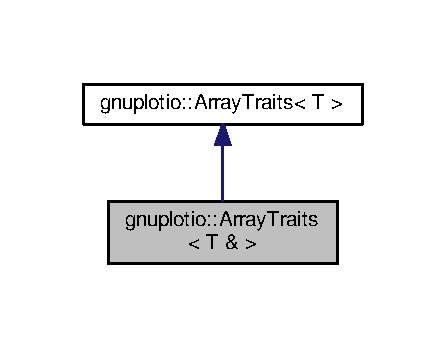
\includegraphics[width=214pt]{classgnuplotio_1_1_array_traits_3_01_t_01_6_01_4__inherit__graph}
\end{center}
\end{figure}


Collaboration diagram for gnuplotio\+:\+:Array\+Traits$<$ T \& $>$\+:
\nopagebreak
\begin{figure}[H]
\begin{center}
\leavevmode
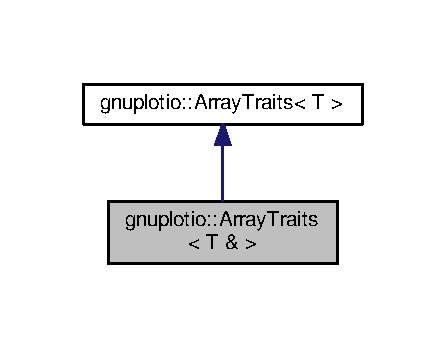
\includegraphics[width=214pt]{classgnuplotio_1_1_array_traits_3_01_t_01_6_01_4__coll__graph}
\end{center}
\end{figure}
\subsection*{Additional Inherited Members}


The documentation for this class was generated from the following file\+:\begin{DoxyCompactItemize}
\item 
/home/rajshinde/\+G\+M\+O\+C\+K/\+Robot\+\_\+\+Controller\+\_\+\+Module/include/gnuplot-\/iostream.\+h\end{DoxyCompactItemize}

\hypertarget{classgnuplotio_1_1_array_traits_3_01_t_00_01typename_01boost_1_1enable__if_3_01boost_1_1mpl_1_1a8de3a8fe198d85f7f5d28b9a2f5bf229}{}\section{gnuplotio\+:\+:Array\+Traits$<$ T, typename boost\+:\+:enable\+\_\+if$<$ boost\+:\+:mpl\+:\+:and\+\_\+$<$ is\+\_\+boost\+\_\+tuple$<$ T $>$, boost\+:\+:mpl\+:\+:not\+\_\+$<$ is\+\_\+boost\+\_\+tuple\+\_\+nulltype$<$ typename T\+:\+:tail\+\_\+type $>$ $>$ $>$ $>$\+:\+:type $>$ Class Template Reference}
\label{classgnuplotio_1_1_array_traits_3_01_t_00_01typename_01boost_1_1enable__if_3_01boost_1_1mpl_1_1a8de3a8fe198d85f7f5d28b9a2f5bf229}\index{gnuplotio\+::\+Array\+Traits$<$ T, typename boost\+::enable\+\_\+if$<$ boost\+::mpl\+::and\+\_\+$<$ is\+\_\+boost\+\_\+tuple$<$ T $>$, boost\+::mpl\+::not\+\_\+$<$ is\+\_\+boost\+\_\+tuple\+\_\+nulltype$<$ typename T\+::tail\+\_\+type $>$ $>$ $>$ $>$\+::type $>$@{gnuplotio\+::\+Array\+Traits$<$ T, typename boost\+::enable\+\_\+if$<$ boost\+::mpl\+::and\+\_\+$<$ is\+\_\+boost\+\_\+tuple$<$ T $>$, boost\+::mpl\+::not\+\_\+$<$ is\+\_\+boost\+\_\+tuple\+\_\+nulltype$<$ typename T\+::tail\+\_\+type $>$ $>$ $>$ $>$\+::type $>$}}


Inheritance diagram for gnuplotio\+:\+:Array\+Traits$<$ T, typename boost\+:\+:enable\+\_\+if$<$ boost\+:\+:mpl\+:\+:and\+\_\+$<$ is\+\_\+boost\+\_\+tuple$<$ T $>$, boost\+:\+:mpl\+:\+:not\+\_\+$<$ is\+\_\+boost\+\_\+tuple\+\_\+nulltype$<$ typename T\+:\+:tail\+\_\+type $>$ $>$ $>$ $>$\+:\+:type $>$\+:
\nopagebreak
\begin{figure}[H]
\begin{center}
\leavevmode
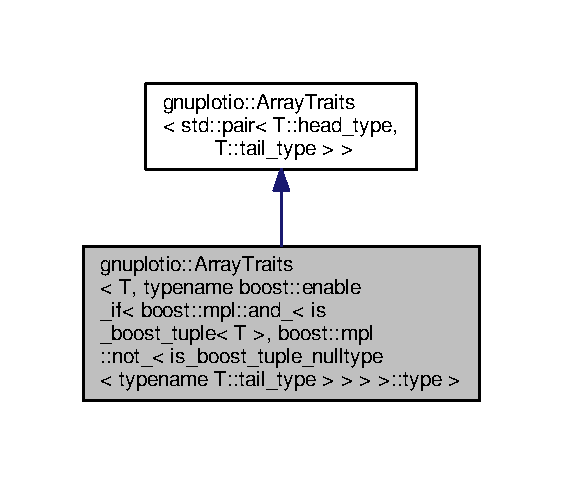
\includegraphics[width=270pt]{classgnuplotio_1_1_array_traits_3_01_t_00_01typename_01boost_1_1enable__if_3_01boost_1_1mpl_1_1a1581fe615c30084043274cbfdd41a619}
\end{center}
\end{figure}


Collaboration diagram for gnuplotio\+:\+:Array\+Traits$<$ T, typename boost\+:\+:enable\+\_\+if$<$ boost\+:\+:mpl\+:\+:and\+\_\+$<$ is\+\_\+boost\+\_\+tuple$<$ T $>$, boost\+:\+:mpl\+:\+:not\+\_\+$<$ is\+\_\+boost\+\_\+tuple\+\_\+nulltype$<$ typename T\+:\+:tail\+\_\+type $>$ $>$ $>$ $>$\+:\+:type $>$\+:
\nopagebreak
\begin{figure}[H]
\begin{center}
\leavevmode
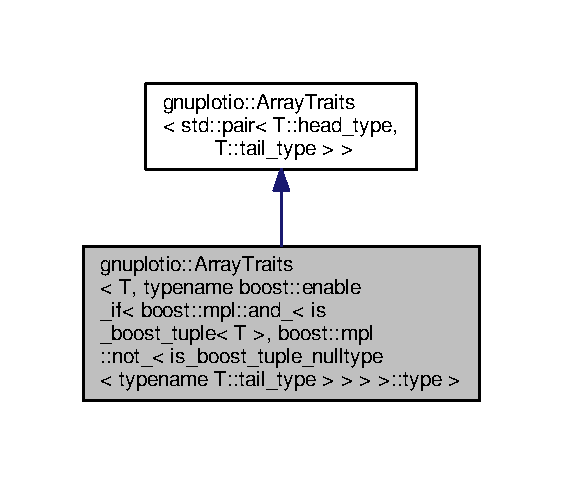
\includegraphics[width=270pt]{classgnuplotio_1_1_array_traits_3_01_t_00_01typename_01boost_1_1enable__if_3_01boost_1_1mpl_1_1aba4443da019311cdd4c31f059136bc6c}
\end{center}
\end{figure}
\subsection*{Public Types}
\begin{DoxyCompactItemize}
\item 
typedef T\+::head\+\_\+type {\bfseries HT}\hypertarget{classgnuplotio_1_1_array_traits_3_01_t_00_01typename_01boost_1_1enable__if_3_01boost_1_1mpl_1_1a8de3a8fe198d85f7f5d28b9a2f5bf229_ab56761f05b74be318cc7becbc59348df}{}\label{classgnuplotio_1_1_array_traits_3_01_t_00_01typename_01boost_1_1enable__if_3_01boost_1_1mpl_1_1a8de3a8fe198d85f7f5d28b9a2f5bf229_ab56761f05b74be318cc7becbc59348df}

\item 
typedef T\+::tail\+\_\+type {\bfseries TT}\hypertarget{classgnuplotio_1_1_array_traits_3_01_t_00_01typename_01boost_1_1enable__if_3_01boost_1_1mpl_1_1a8de3a8fe198d85f7f5d28b9a2f5bf229_a16316f598ab57b0b7ceea99dcd34632e}{}\label{classgnuplotio_1_1_array_traits_3_01_t_00_01typename_01boost_1_1enable__if_3_01boost_1_1mpl_1_1a8de3a8fe198d85f7f5d28b9a2f5bf229_a16316f598ab57b0b7ceea99dcd34632e}

\item 
typedef \hyperlink{classgnuplotio_1_1_array_traits}{Array\+Traits}$<$ typename std\+::pair$<$ HT, TT $>$ $>$ {\bfseries parent}\hypertarget{classgnuplotio_1_1_array_traits_3_01_t_00_01typename_01boost_1_1enable__if_3_01boost_1_1mpl_1_1a8de3a8fe198d85f7f5d28b9a2f5bf229_aad44f59a1d618b863442a9fdaa83d142}{}\label{classgnuplotio_1_1_array_traits_3_01_t_00_01typename_01boost_1_1enable__if_3_01boost_1_1mpl_1_1a8de3a8fe198d85f7f5d28b9a2f5bf229_aad44f59a1d618b863442a9fdaa83d142}

\end{DoxyCompactItemize}
\subsection*{Static Public Member Functions}
\begin{DoxyCompactItemize}
\item 
static \hyperlink{structgnuplotio_1_1_error___was_not_container}{parent\+::range\+\_\+type} {\bfseries get\+\_\+range} (const T \&arg)\hypertarget{classgnuplotio_1_1_array_traits_3_01_t_00_01typename_01boost_1_1enable__if_3_01boost_1_1mpl_1_1a8de3a8fe198d85f7f5d28b9a2f5bf229_aec07e01edbb46f5f283d5b6af068c0f2}{}\label{classgnuplotio_1_1_array_traits_3_01_t_00_01typename_01boost_1_1enable__if_3_01boost_1_1mpl_1_1a8de3a8fe198d85f7f5d28b9a2f5bf229_aec07e01edbb46f5f283d5b6af068c0f2}

\end{DoxyCompactItemize}
\subsection*{Additional Inherited Members}


The documentation for this class was generated from the following file\+:\begin{DoxyCompactItemize}
\item 
/home/rajshinde/\+G\+M\+O\+C\+K/\+Robot\+\_\+\+Controller\+\_\+\+Module/include/gnuplot-\/iostream.\+h\end{DoxyCompactItemize}

\hypertarget{classgnuplotio_1_1_array_traits_3_01_t_00_01typename_01boost_1_1enable__if_3_01boost_1_1mpl_1_1ad3fa8e75dccbaae12a06d17831678a88}{}\section{gnuplotio\+:\+:Array\+Traits$<$ T, typename boost\+:\+:enable\+\_\+if$<$ boost\+:\+:mpl\+:\+:and\+\_\+$<$ is\+\_\+boost\+\_\+tuple$<$ T $>$, is\+\_\+boost\+\_\+tuple\+\_\+nulltype$<$ typename T\+:\+:tail\+\_\+type $>$ $>$ $>$\+:\+:type $>$ Class Template Reference}
\label{classgnuplotio_1_1_array_traits_3_01_t_00_01typename_01boost_1_1enable__if_3_01boost_1_1mpl_1_1ad3fa8e75dccbaae12a06d17831678a88}\index{gnuplotio\+::\+Array\+Traits$<$ T, typename boost\+::enable\+\_\+if$<$ boost\+::mpl\+::and\+\_\+$<$ is\+\_\+boost\+\_\+tuple$<$ T $>$, is\+\_\+boost\+\_\+tuple\+\_\+nulltype$<$ typename T\+::tail\+\_\+type $>$ $>$ $>$\+::type $>$@{gnuplotio\+::\+Array\+Traits$<$ T, typename boost\+::enable\+\_\+if$<$ boost\+::mpl\+::and\+\_\+$<$ is\+\_\+boost\+\_\+tuple$<$ T $>$, is\+\_\+boost\+\_\+tuple\+\_\+nulltype$<$ typename T\+::tail\+\_\+type $>$ $>$ $>$\+::type $>$}}


Inheritance diagram for gnuplotio\+:\+:Array\+Traits$<$ T, typename boost\+:\+:enable\+\_\+if$<$ boost\+:\+:mpl\+:\+:and\+\_\+$<$ is\+\_\+boost\+\_\+tuple$<$ T $>$, is\+\_\+boost\+\_\+tuple\+\_\+nulltype$<$ typename T\+:\+:tail\+\_\+type $>$ $>$ $>$\+:\+:type $>$\+:
\nopagebreak
\begin{figure}[H]
\begin{center}
\leavevmode
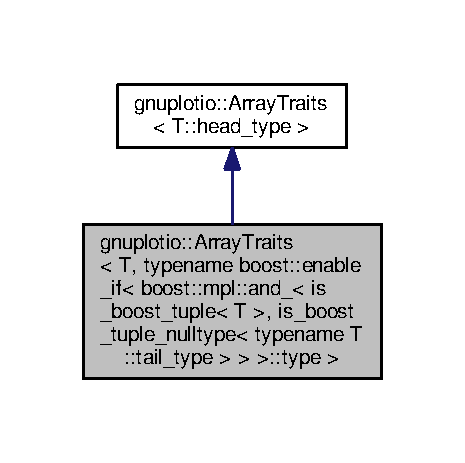
\includegraphics[width=223pt]{classgnuplotio_1_1_array_traits_3_01_t_00_01typename_01boost_1_1enable__if_3_01boost_1_1mpl_1_1aea65f5b28bab149b37099425ffdc1482}
\end{center}
\end{figure}


Collaboration diagram for gnuplotio\+:\+:Array\+Traits$<$ T, typename boost\+:\+:enable\+\_\+if$<$ boost\+:\+:mpl\+:\+:and\+\_\+$<$ is\+\_\+boost\+\_\+tuple$<$ T $>$, is\+\_\+boost\+\_\+tuple\+\_\+nulltype$<$ typename T\+:\+:tail\+\_\+type $>$ $>$ $>$\+:\+:type $>$\+:
\nopagebreak
\begin{figure}[H]
\begin{center}
\leavevmode
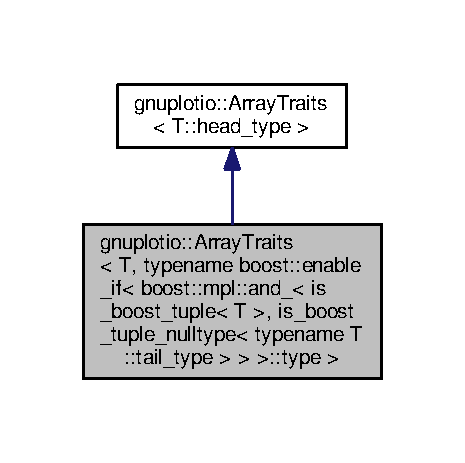
\includegraphics[width=223pt]{classgnuplotio_1_1_array_traits_3_01_t_00_01typename_01boost_1_1enable__if_3_01boost_1_1mpl_1_1a7c2880846d33bb3586d5921312165f33}
\end{center}
\end{figure}
\subsection*{Static Public Member Functions}
\begin{DoxyCompactItemize}
\item 
static \hyperlink{structgnuplotio_1_1_error___was_not_container}{parent\+::range\+\_\+type} {\bfseries get\+\_\+range} (const T \&arg)\hypertarget{classgnuplotio_1_1_array_traits_3_01_t_00_01typename_01boost_1_1enable__if_3_01boost_1_1mpl_1_1ad3fa8e75dccbaae12a06d17831678a88_ad0485dd16a9d54a4eb75bf3e75b1facd}{}\label{classgnuplotio_1_1_array_traits_3_01_t_00_01typename_01boost_1_1enable__if_3_01boost_1_1mpl_1_1ad3fa8e75dccbaae12a06d17831678a88_ad0485dd16a9d54a4eb75bf3e75b1facd}

\end{DoxyCompactItemize}
\subsection*{Additional Inherited Members}


The documentation for this class was generated from the following file\+:\begin{DoxyCompactItemize}
\item 
/home/rajshinde/\+G\+M\+O\+C\+K/\+Robot\+\_\+\+Controller\+\_\+\+Module/include/gnuplot-\/iostream.\+h\end{DoxyCompactItemize}

\hypertarget{classgnuplotio_1_1_array_traits_3_01_t_00_01typename_01boost_1_1enable__if_3_01is__like__stl__co9e1736bbd08cd58c6993ab613a998887}{}\section{gnuplotio\+:\+:Array\+Traits$<$ T, typename boost\+:\+:enable\+\_\+if$<$ is\+\_\+like\+\_\+stl\+\_\+container$<$ T $>$ $>$\+:\+:type $>$ Class Template Reference}
\label{classgnuplotio_1_1_array_traits_3_01_t_00_01typename_01boost_1_1enable__if_3_01is__like__stl__co9e1736bbd08cd58c6993ab613a998887}\index{gnuplotio\+::\+Array\+Traits$<$ T, typename boost\+::enable\+\_\+if$<$ is\+\_\+like\+\_\+stl\+\_\+container$<$ T $>$ $>$\+::type $>$@{gnuplotio\+::\+Array\+Traits$<$ T, typename boost\+::enable\+\_\+if$<$ is\+\_\+like\+\_\+stl\+\_\+container$<$ T $>$ $>$\+::type $>$}}


Inheritance diagram for gnuplotio\+:\+:Array\+Traits$<$ T, typename boost\+:\+:enable\+\_\+if$<$ is\+\_\+like\+\_\+stl\+\_\+container$<$ T $>$ $>$\+:\+:type $>$\+:
\nopagebreak
\begin{figure}[H]
\begin{center}
\leavevmode
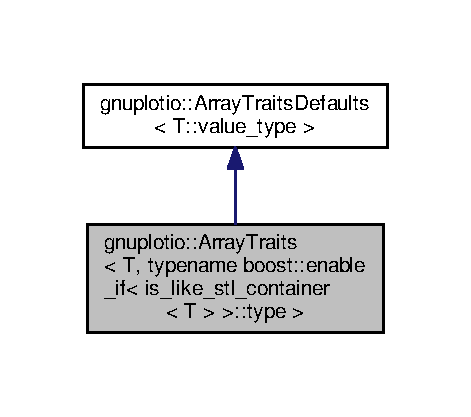
\includegraphics[width=226pt]{classgnuplotio_1_1_array_traits_3_01_t_00_01typename_01boost_1_1enable__if_3_01is__like__stl__co39a918c94e39b553da961d4c081ad747}
\end{center}
\end{figure}


Collaboration diagram for gnuplotio\+:\+:Array\+Traits$<$ T, typename boost\+:\+:enable\+\_\+if$<$ is\+\_\+like\+\_\+stl\+\_\+container$<$ T $>$ $>$\+:\+:type $>$\+:
\nopagebreak
\begin{figure}[H]
\begin{center}
\leavevmode
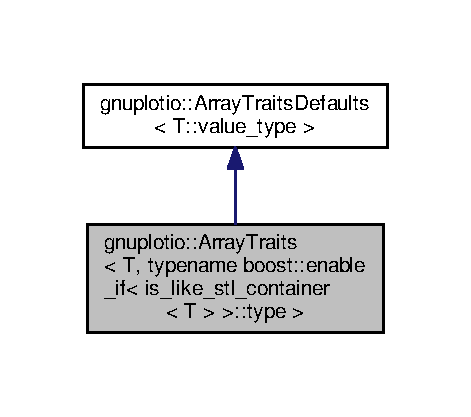
\includegraphics[width=226pt]{classgnuplotio_1_1_array_traits_3_01_t_00_01typename_01boost_1_1enable__if_3_01is__like__stl__coea0859b06c932ef4cd47658c6683d98b}
\end{center}
\end{figure}
\subsection*{Public Types}
\begin{DoxyCompactItemize}
\item 
typedef \hyperlink{classgnuplotio_1_1_iterator_range}{Iterator\+Range}$<$ typename T\+::const\+\_\+iterator, typename T\+::value\+\_\+type $>$ {\bfseries range\+\_\+type}\hypertarget{classgnuplotio_1_1_array_traits_3_01_t_00_01typename_01boost_1_1enable__if_3_01is__like__stl__co9e1736bbd08cd58c6993ab613a998887_ab702072abbe018bbc90b9967ca8c4b42}{}\label{classgnuplotio_1_1_array_traits_3_01_t_00_01typename_01boost_1_1enable__if_3_01is__like__stl__co9e1736bbd08cd58c6993ab613a998887_ab702072abbe018bbc90b9967ca8c4b42}

\end{DoxyCompactItemize}
\subsection*{Static Public Member Functions}
\begin{DoxyCompactItemize}
\item 
static \hyperlink{classgnuplotio_1_1_iterator_range}{range\+\_\+type} {\bfseries get\+\_\+range} (const T \&arg)\hypertarget{classgnuplotio_1_1_array_traits_3_01_t_00_01typename_01boost_1_1enable__if_3_01is__like__stl__co9e1736bbd08cd58c6993ab613a998887_a89d4150ab3c479cde972071a10acd27b}{}\label{classgnuplotio_1_1_array_traits_3_01_t_00_01typename_01boost_1_1enable__if_3_01is__like__stl__co9e1736bbd08cd58c6993ab613a998887_a89d4150ab3c479cde972071a10acd27b}

\end{DoxyCompactItemize}
\subsection*{Additional Inherited Members}


The documentation for this class was generated from the following file\+:\begin{DoxyCompactItemize}
\item 
/home/rajshinde/\+G\+M\+O\+C\+K/\+Robot\+\_\+\+Controller\+\_\+\+Module/include/gnuplot-\/iostream.\+h\end{DoxyCompactItemize}

\hypertarget{classgnuplotio_1_1_array_traits_3_01_t[_n]_4}{}\section{gnuplotio\+:\+:Array\+Traits$<$ T\mbox{[}N\mbox{]}$>$ Class Template Reference}
\label{classgnuplotio_1_1_array_traits_3_01_t[_n]_4}\index{gnuplotio\+::\+Array\+Traits$<$ T\mbox{[}\+N\mbox{]}$>$@{gnuplotio\+::\+Array\+Traits$<$ T[N]$>$}}


Inheritance diagram for gnuplotio\+:\+:Array\+Traits$<$ T\mbox{[}N\mbox{]}$>$\+:
\nopagebreak
\begin{figure}[H]
\begin{center}
\leavevmode
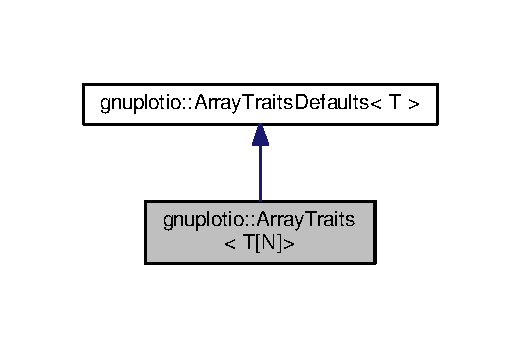
\includegraphics[width=250pt]{classgnuplotio_1_1_array_traits_3_01_t[_n]_4__inherit__graph}
\end{center}
\end{figure}


Collaboration diagram for gnuplotio\+:\+:Array\+Traits$<$ T\mbox{[}N\mbox{]}$>$\+:
\nopagebreak
\begin{figure}[H]
\begin{center}
\leavevmode
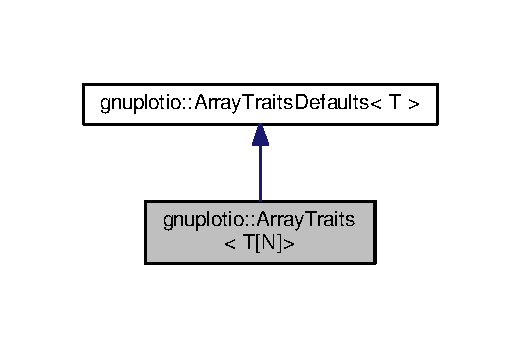
\includegraphics[width=250pt]{classgnuplotio_1_1_array_traits_3_01_t[_n]_4__coll__graph}
\end{center}
\end{figure}
\subsection*{Public Types}
\begin{DoxyCompactItemize}
\item 
typedef \hyperlink{classgnuplotio_1_1_iterator_range}{Iterator\+Range}$<$ const T $\ast$, T $>$ {\bfseries range\+\_\+type}\hypertarget{classgnuplotio_1_1_array_traits_3_01_t[_n]_4_a926f3c3d14fbe82aab7b70ccc16d20fb}{}\label{classgnuplotio_1_1_array_traits_3_01_t[_n]_4_a926f3c3d14fbe82aab7b70ccc16d20fb}

\end{DoxyCompactItemize}
\subsection*{Static Public Member Functions}
\begin{DoxyCompactItemize}
\item 
static \hyperlink{classgnuplotio_1_1_iterator_range}{range\+\_\+type} {\bfseries get\+\_\+range} (const T(\&arg)\mbox{[}N\mbox{]})\hypertarget{classgnuplotio_1_1_array_traits_3_01_t[_n]_4_adc9c1ce6da4923418f367e08c150a928}{}\label{classgnuplotio_1_1_array_traits_3_01_t[_n]_4_adc9c1ce6da4923418f367e08c150a928}

\end{DoxyCompactItemize}
\subsection*{Additional Inherited Members}


The documentation for this class was generated from the following file\+:\begin{DoxyCompactItemize}
\item 
/home/rajshinde/\+G\+M\+O\+C\+K/\+Robot\+\_\+\+Controller\+\_\+\+Module/include/gnuplot-\/iostream.\+h\end{DoxyCompactItemize}

\hypertarget{classgnuplotio_1_1_array_traits_defaults}{}\section{gnuplotio\+:\+:Array\+Traits\+Defaults$<$ V $>$ Class Template Reference}
\label{classgnuplotio_1_1_array_traits_defaults}\index{gnuplotio\+::\+Array\+Traits\+Defaults$<$ V $>$@{gnuplotio\+::\+Array\+Traits\+Defaults$<$ V $>$}}
\subsection*{Public Types}
\begin{DoxyCompactItemize}
\item 
typedef V {\bfseries value\+\_\+type}\hypertarget{classgnuplotio_1_1_array_traits_defaults_ad7a9e8d19419fabe2ab9cc1b76c9965b}{}\label{classgnuplotio_1_1_array_traits_defaults_ad7a9e8d19419fabe2ab9cc1b76c9965b}

\end{DoxyCompactItemize}
\subsection*{Static Public Attributes}
\begin{DoxyCompactItemize}
\item 
static const bool {\bfseries is\+\_\+container} = true\hypertarget{classgnuplotio_1_1_array_traits_defaults_a57bab5bf3617f0ee66fdd4dcb751aa21}{}\label{classgnuplotio_1_1_array_traits_defaults_a57bab5bf3617f0ee66fdd4dcb751aa21}

\item 
static const bool {\bfseries allow\+\_\+auto\+\_\+unwrap} = true\hypertarget{classgnuplotio_1_1_array_traits_defaults_ac8d430cba6ceefc6f52706455f12a0e8}{}\label{classgnuplotio_1_1_array_traits_defaults_ac8d430cba6ceefc6f52706455f12a0e8}

\item 
static const size\+\_\+t {\bfseries depth} = \hyperlink{classgnuplotio_1_1_array_traits}{Array\+Traits}$<$V$>$\+::depth + 1\hypertarget{classgnuplotio_1_1_array_traits_defaults_ac51367f5da9096249b162af1496e36ab}{}\label{classgnuplotio_1_1_array_traits_defaults_ac51367f5da9096249b162af1496e36ab}

\end{DoxyCompactItemize}


The documentation for this class was generated from the following file\+:\begin{DoxyCompactItemize}
\item 
/home/rajshinde/\+G\+M\+O\+C\+K/\+Robot\+\_\+\+Controller\+\_\+\+Module/include/gnuplot-\/iostream.\+h\end{DoxyCompactItemize}

\hypertarget{structgnuplotio_1_1_binary_sender}{}\section{gnuplotio\+:\+:Binary\+Sender$<$ T, Enable $>$ Struct Template Reference}
\label{structgnuplotio_1_1_binary_sender}\index{gnuplotio\+::\+Binary\+Sender$<$ T, Enable $>$@{gnuplotio\+::\+Binary\+Sender$<$ T, Enable $>$}}
\subsection*{Public Member Functions}
\begin{DoxyCompactItemize}
\item 
{\bfseries G\+N\+U\+P\+L\+O\+T\+\_\+\+S\+T\+A\+T\+I\+C\+\_\+\+A\+S\+S\+E\+R\+T\+\_\+\+M\+SG} ((sizeof(T)==0),\char`\"{}Binary\+Sender class not specialized for this type\char`\"{})\hypertarget{structgnuplotio_1_1_binary_sender_a165c59a28adc4a90930925c6e0bfb0a9}{}\label{structgnuplotio_1_1_binary_sender_a165c59a28adc4a90930925c6e0bfb0a9}

\end{DoxyCompactItemize}
\subsection*{Static Public Member Functions}
\begin{DoxyCompactItemize}
\item 
static void {\bfseries send} (std\+::ostream \&stream, const T \&v)\hypertarget{structgnuplotio_1_1_binary_sender_a4b5dd22b7679c4f0ce4d8e75b36c8a21}{}\label{structgnuplotio_1_1_binary_sender_a4b5dd22b7679c4f0ce4d8e75b36c8a21}

\end{DoxyCompactItemize}


The documentation for this struct was generated from the following file\+:\begin{DoxyCompactItemize}
\item 
/home/rajshinde/\+G\+M\+O\+C\+K/\+Robot\+\_\+\+Controller\+\_\+\+Module/include/gnuplot-\/iostream.\+h\end{DoxyCompactItemize}

\hypertarget{structgnuplotio_1_1_binary_sender_3_01boost_1_1int16__t_01_4}{}\section{gnuplotio\+:\+:Binary\+Sender$<$ boost\+:\+:int16\+\_\+t $>$ Struct Template Reference}
\label{structgnuplotio_1_1_binary_sender_3_01boost_1_1int16__t_01_4}\index{gnuplotio\+::\+Binary\+Sender$<$ boost\+::int16\+\_\+t $>$@{gnuplotio\+::\+Binary\+Sender$<$ boost\+::int16\+\_\+t $>$}}


Inheritance diagram for gnuplotio\+:\+:Binary\+Sender$<$ boost\+:\+:int16\+\_\+t $>$\+:
\nopagebreak
\begin{figure}[H]
\begin{center}
\leavevmode
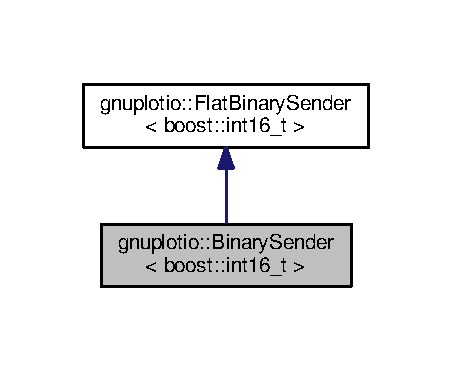
\includegraphics[width=217pt]{structgnuplotio_1_1_binary_sender_3_01boost_1_1int16__t_01_4__inherit__graph}
\end{center}
\end{figure}


Collaboration diagram for gnuplotio\+:\+:Binary\+Sender$<$ boost\+:\+:int16\+\_\+t $>$\+:
\nopagebreak
\begin{figure}[H]
\begin{center}
\leavevmode
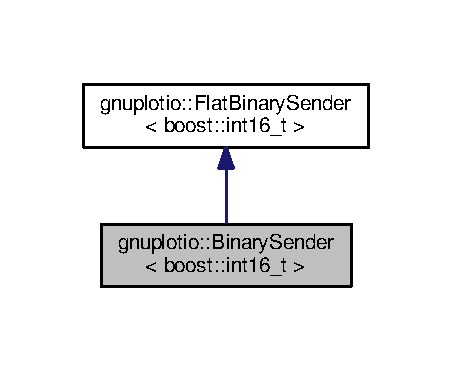
\includegraphics[width=217pt]{structgnuplotio_1_1_binary_sender_3_01boost_1_1int16__t_01_4__coll__graph}
\end{center}
\end{figure}
\subsection*{Additional Inherited Members}


The documentation for this struct was generated from the following file\+:\begin{DoxyCompactItemize}
\item 
/home/rajshinde/\+G\+M\+O\+C\+K/\+Robot\+\_\+\+Controller\+\_\+\+Module/include/gnuplot-\/iostream.\+h\end{DoxyCompactItemize}

\hypertarget{structgnuplotio_1_1_binary_sender_3_01boost_1_1int32__t_01_4}{}\section{gnuplotio\+:\+:Binary\+Sender$<$ boost\+:\+:int32\+\_\+t $>$ Struct Template Reference}
\label{structgnuplotio_1_1_binary_sender_3_01boost_1_1int32__t_01_4}\index{gnuplotio\+::\+Binary\+Sender$<$ boost\+::int32\+\_\+t $>$@{gnuplotio\+::\+Binary\+Sender$<$ boost\+::int32\+\_\+t $>$}}


Inheritance diagram for gnuplotio\+:\+:Binary\+Sender$<$ boost\+:\+:int32\+\_\+t $>$\+:
\nopagebreak
\begin{figure}[H]
\begin{center}
\leavevmode
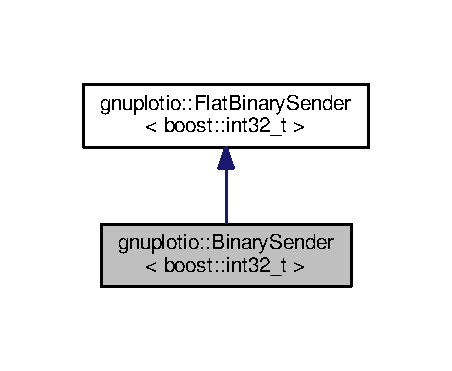
\includegraphics[width=217pt]{structgnuplotio_1_1_binary_sender_3_01boost_1_1int32__t_01_4__inherit__graph}
\end{center}
\end{figure}


Collaboration diagram for gnuplotio\+:\+:Binary\+Sender$<$ boost\+:\+:int32\+\_\+t $>$\+:
\nopagebreak
\begin{figure}[H]
\begin{center}
\leavevmode
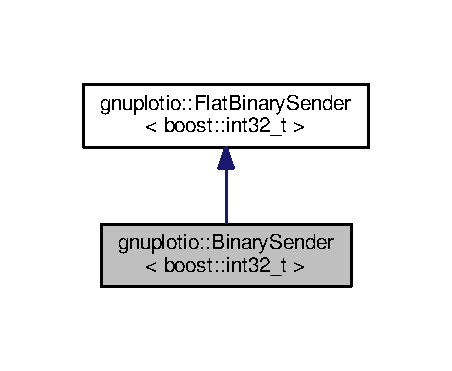
\includegraphics[width=217pt]{structgnuplotio_1_1_binary_sender_3_01boost_1_1int32__t_01_4__coll__graph}
\end{center}
\end{figure}
\subsection*{Additional Inherited Members}


The documentation for this struct was generated from the following file\+:\begin{DoxyCompactItemize}
\item 
/home/rajshinde/\+G\+M\+O\+C\+K/\+Robot\+\_\+\+Controller\+\_\+\+Module/include/gnuplot-\/iostream.\+h\end{DoxyCompactItemize}

\hypertarget{structgnuplotio_1_1_binary_sender_3_01boost_1_1int64__t_01_4}{}\section{gnuplotio\+:\+:Binary\+Sender$<$ boost\+:\+:int64\+\_\+t $>$ Struct Template Reference}
\label{structgnuplotio_1_1_binary_sender_3_01boost_1_1int64__t_01_4}\index{gnuplotio\+::\+Binary\+Sender$<$ boost\+::int64\+\_\+t $>$@{gnuplotio\+::\+Binary\+Sender$<$ boost\+::int64\+\_\+t $>$}}


Inheritance diagram for gnuplotio\+:\+:Binary\+Sender$<$ boost\+:\+:int64\+\_\+t $>$\+:
\nopagebreak
\begin{figure}[H]
\begin{center}
\leavevmode
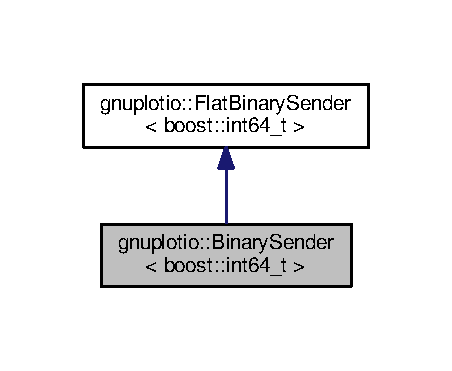
\includegraphics[width=217pt]{structgnuplotio_1_1_binary_sender_3_01boost_1_1int64__t_01_4__inherit__graph}
\end{center}
\end{figure}


Collaboration diagram for gnuplotio\+:\+:Binary\+Sender$<$ boost\+:\+:int64\+\_\+t $>$\+:
\nopagebreak
\begin{figure}[H]
\begin{center}
\leavevmode
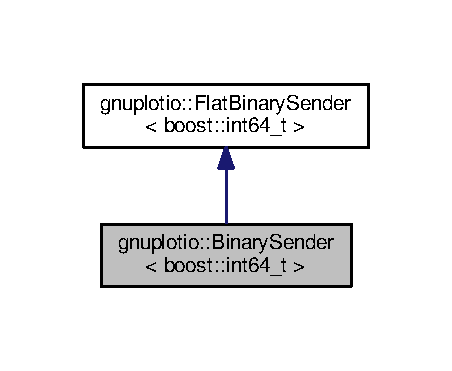
\includegraphics[width=217pt]{structgnuplotio_1_1_binary_sender_3_01boost_1_1int64__t_01_4__coll__graph}
\end{center}
\end{figure}
\subsection*{Additional Inherited Members}


The documentation for this struct was generated from the following file\+:\begin{DoxyCompactItemize}
\item 
/home/rajshinde/\+G\+M\+O\+C\+K/\+Robot\+\_\+\+Controller\+\_\+\+Module/include/gnuplot-\/iostream.\+h\end{DoxyCompactItemize}

\hypertarget{structgnuplotio_1_1_binary_sender_3_01boost_1_1int8__t_01_4}{}\section{gnuplotio\+:\+:Binary\+Sender$<$ boost\+:\+:int8\+\_\+t $>$ Struct Template Reference}
\label{structgnuplotio_1_1_binary_sender_3_01boost_1_1int8__t_01_4}\index{gnuplotio\+::\+Binary\+Sender$<$ boost\+::int8\+\_\+t $>$@{gnuplotio\+::\+Binary\+Sender$<$ boost\+::int8\+\_\+t $>$}}


Inheritance diagram for gnuplotio\+:\+:Binary\+Sender$<$ boost\+:\+:int8\+\_\+t $>$\+:
\nopagebreak
\begin{figure}[H]
\begin{center}
\leavevmode
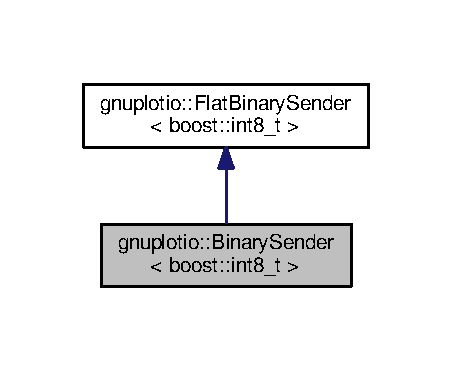
\includegraphics[width=217pt]{structgnuplotio_1_1_binary_sender_3_01boost_1_1int8__t_01_4__inherit__graph}
\end{center}
\end{figure}


Collaboration diagram for gnuplotio\+:\+:Binary\+Sender$<$ boost\+:\+:int8\+\_\+t $>$\+:
\nopagebreak
\begin{figure}[H]
\begin{center}
\leavevmode
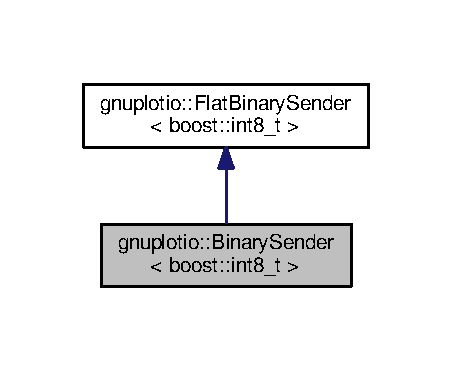
\includegraphics[width=217pt]{structgnuplotio_1_1_binary_sender_3_01boost_1_1int8__t_01_4__coll__graph}
\end{center}
\end{figure}
\subsection*{Additional Inherited Members}


The documentation for this struct was generated from the following file\+:\begin{DoxyCompactItemize}
\item 
/home/rajshinde/\+G\+M\+O\+C\+K/\+Robot\+\_\+\+Controller\+\_\+\+Module/include/gnuplot-\/iostream.\+h\end{DoxyCompactItemize}

\hypertarget{structgnuplotio_1_1_binary_sender_3_01boost_1_1uint16__t_01_4}{}\section{gnuplotio\+:\+:Binary\+Sender$<$ boost\+:\+:uint16\+\_\+t $>$ Struct Template Reference}
\label{structgnuplotio_1_1_binary_sender_3_01boost_1_1uint16__t_01_4}\index{gnuplotio\+::\+Binary\+Sender$<$ boost\+::uint16\+\_\+t $>$@{gnuplotio\+::\+Binary\+Sender$<$ boost\+::uint16\+\_\+t $>$}}


Inheritance diagram for gnuplotio\+:\+:Binary\+Sender$<$ boost\+:\+:uint16\+\_\+t $>$\+:
\nopagebreak
\begin{figure}[H]
\begin{center}
\leavevmode
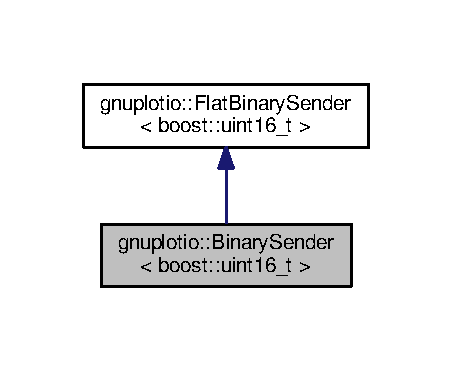
\includegraphics[width=217pt]{structgnuplotio_1_1_binary_sender_3_01boost_1_1uint16__t_01_4__inherit__graph}
\end{center}
\end{figure}


Collaboration diagram for gnuplotio\+:\+:Binary\+Sender$<$ boost\+:\+:uint16\+\_\+t $>$\+:
\nopagebreak
\begin{figure}[H]
\begin{center}
\leavevmode
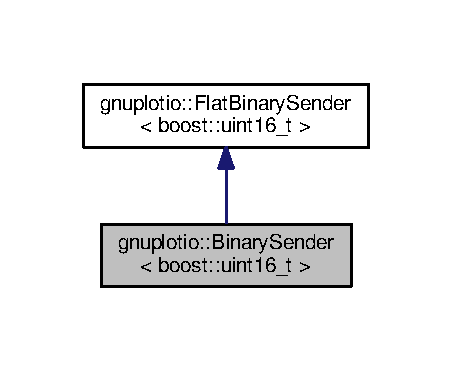
\includegraphics[width=217pt]{structgnuplotio_1_1_binary_sender_3_01boost_1_1uint16__t_01_4__coll__graph}
\end{center}
\end{figure}
\subsection*{Additional Inherited Members}


The documentation for this struct was generated from the following file\+:\begin{DoxyCompactItemize}
\item 
/home/rajshinde/\+G\+M\+O\+C\+K/\+Robot\+\_\+\+Controller\+\_\+\+Module/include/gnuplot-\/iostream.\+h\end{DoxyCompactItemize}

\hypertarget{structgnuplotio_1_1_binary_sender_3_01boost_1_1uint32__t_01_4}{}\section{gnuplotio\+:\+:Binary\+Sender$<$ boost\+:\+:uint32\+\_\+t $>$ Struct Template Reference}
\label{structgnuplotio_1_1_binary_sender_3_01boost_1_1uint32__t_01_4}\index{gnuplotio\+::\+Binary\+Sender$<$ boost\+::uint32\+\_\+t $>$@{gnuplotio\+::\+Binary\+Sender$<$ boost\+::uint32\+\_\+t $>$}}


Inheritance diagram for gnuplotio\+:\+:Binary\+Sender$<$ boost\+:\+:uint32\+\_\+t $>$\+:
\nopagebreak
\begin{figure}[H]
\begin{center}
\leavevmode
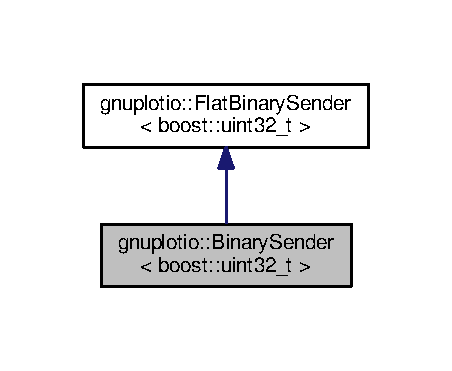
\includegraphics[width=217pt]{structgnuplotio_1_1_binary_sender_3_01boost_1_1uint32__t_01_4__inherit__graph}
\end{center}
\end{figure}


Collaboration diagram for gnuplotio\+:\+:Binary\+Sender$<$ boost\+:\+:uint32\+\_\+t $>$\+:
\nopagebreak
\begin{figure}[H]
\begin{center}
\leavevmode
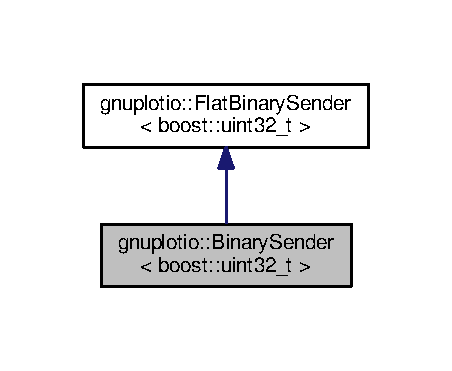
\includegraphics[width=217pt]{structgnuplotio_1_1_binary_sender_3_01boost_1_1uint32__t_01_4__coll__graph}
\end{center}
\end{figure}
\subsection*{Additional Inherited Members}


The documentation for this struct was generated from the following file\+:\begin{DoxyCompactItemize}
\item 
/home/rajshinde/\+G\+M\+O\+C\+K/\+Robot\+\_\+\+Controller\+\_\+\+Module/include/gnuplot-\/iostream.\+h\end{DoxyCompactItemize}

\hypertarget{structgnuplotio_1_1_binary_sender_3_01boost_1_1uint64__t_01_4}{}\section{gnuplotio\+:\+:Binary\+Sender$<$ boost\+:\+:uint64\+\_\+t $>$ Struct Template Reference}
\label{structgnuplotio_1_1_binary_sender_3_01boost_1_1uint64__t_01_4}\index{gnuplotio\+::\+Binary\+Sender$<$ boost\+::uint64\+\_\+t $>$@{gnuplotio\+::\+Binary\+Sender$<$ boost\+::uint64\+\_\+t $>$}}


Inheritance diagram for gnuplotio\+:\+:Binary\+Sender$<$ boost\+:\+:uint64\+\_\+t $>$\+:
\nopagebreak
\begin{figure}[H]
\begin{center}
\leavevmode
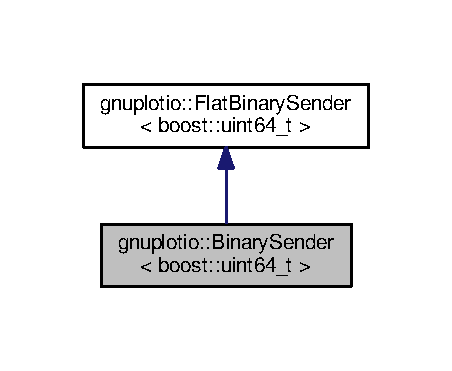
\includegraphics[width=217pt]{structgnuplotio_1_1_binary_sender_3_01boost_1_1uint64__t_01_4__inherit__graph}
\end{center}
\end{figure}


Collaboration diagram for gnuplotio\+:\+:Binary\+Sender$<$ boost\+:\+:uint64\+\_\+t $>$\+:
\nopagebreak
\begin{figure}[H]
\begin{center}
\leavevmode
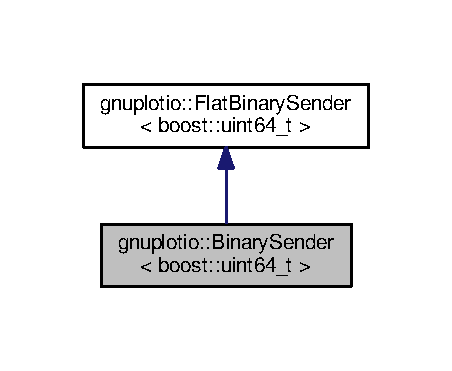
\includegraphics[width=217pt]{structgnuplotio_1_1_binary_sender_3_01boost_1_1uint64__t_01_4__coll__graph}
\end{center}
\end{figure}
\subsection*{Additional Inherited Members}


The documentation for this struct was generated from the following file\+:\begin{DoxyCompactItemize}
\item 
/home/rajshinde/\+G\+M\+O\+C\+K/\+Robot\+\_\+\+Controller\+\_\+\+Module/include/gnuplot-\/iostream.\+h\end{DoxyCompactItemize}

\hypertarget{structgnuplotio_1_1_binary_sender_3_01boost_1_1uint8__t_01_4}{}\section{gnuplotio\+:\+:Binary\+Sender$<$ boost\+:\+:uint8\+\_\+t $>$ Struct Template Reference}
\label{structgnuplotio_1_1_binary_sender_3_01boost_1_1uint8__t_01_4}\index{gnuplotio\+::\+Binary\+Sender$<$ boost\+::uint8\+\_\+t $>$@{gnuplotio\+::\+Binary\+Sender$<$ boost\+::uint8\+\_\+t $>$}}


Inheritance diagram for gnuplotio\+:\+:Binary\+Sender$<$ boost\+:\+:uint8\+\_\+t $>$\+:
\nopagebreak
\begin{figure}[H]
\begin{center}
\leavevmode
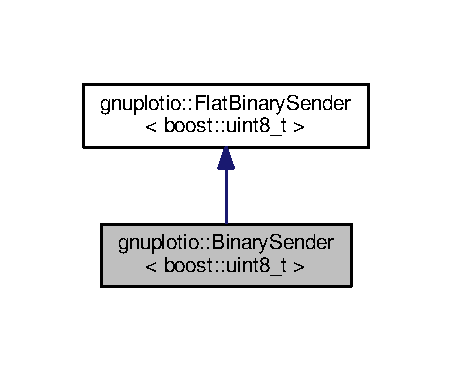
\includegraphics[width=217pt]{structgnuplotio_1_1_binary_sender_3_01boost_1_1uint8__t_01_4__inherit__graph}
\end{center}
\end{figure}


Collaboration diagram for gnuplotio\+:\+:Binary\+Sender$<$ boost\+:\+:uint8\+\_\+t $>$\+:
\nopagebreak
\begin{figure}[H]
\begin{center}
\leavevmode
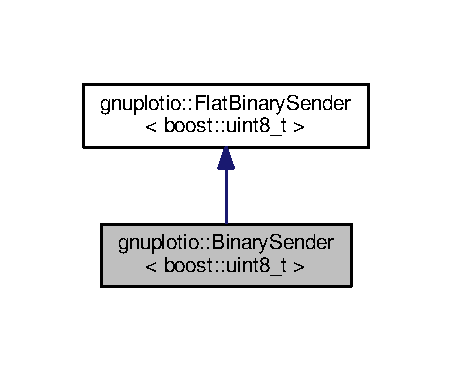
\includegraphics[width=217pt]{structgnuplotio_1_1_binary_sender_3_01boost_1_1uint8__t_01_4__coll__graph}
\end{center}
\end{figure}
\subsection*{Additional Inherited Members}


The documentation for this struct was generated from the following file\+:\begin{DoxyCompactItemize}
\item 
/home/rajshinde/\+G\+M\+O\+C\+K/\+Robot\+\_\+\+Controller\+\_\+\+Module/include/gnuplot-\/iostream.\+h\end{DoxyCompactItemize}

\hypertarget{structgnuplotio_1_1_binary_sender_3_01double_01_4}{}\section{gnuplotio\+:\+:Binary\+Sender$<$ double $>$ Struct Template Reference}
\label{structgnuplotio_1_1_binary_sender_3_01double_01_4}\index{gnuplotio\+::\+Binary\+Sender$<$ double $>$@{gnuplotio\+::\+Binary\+Sender$<$ double $>$}}


Inheritance diagram for gnuplotio\+:\+:Binary\+Sender$<$ double $>$\+:
\nopagebreak
\begin{figure}[H]
\begin{center}
\leavevmode
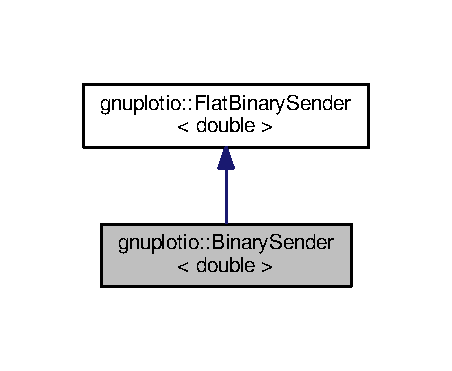
\includegraphics[width=217pt]{structgnuplotio_1_1_binary_sender_3_01double_01_4__inherit__graph}
\end{center}
\end{figure}


Collaboration diagram for gnuplotio\+:\+:Binary\+Sender$<$ double $>$\+:
\nopagebreak
\begin{figure}[H]
\begin{center}
\leavevmode
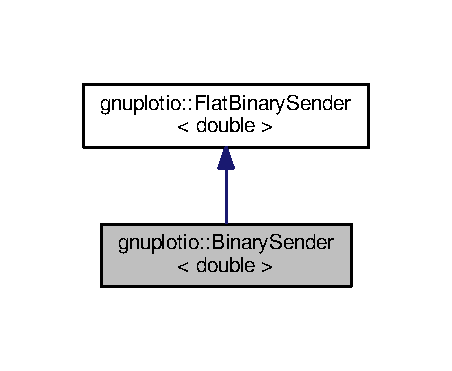
\includegraphics[width=217pt]{structgnuplotio_1_1_binary_sender_3_01double_01_4__coll__graph}
\end{center}
\end{figure}
\subsection*{Additional Inherited Members}


The documentation for this struct was generated from the following file\+:\begin{DoxyCompactItemize}
\item 
/home/rajshinde/\+G\+M\+O\+C\+K/\+Robot\+\_\+\+Controller\+\_\+\+Module/include/gnuplot-\/iostream.\+h\end{DoxyCompactItemize}

\hypertarget{structgnuplotio_1_1_binary_sender_3_01float_01_4}{}\section{gnuplotio\+:\+:Binary\+Sender$<$ float $>$ Struct Template Reference}
\label{structgnuplotio_1_1_binary_sender_3_01float_01_4}\index{gnuplotio\+::\+Binary\+Sender$<$ float $>$@{gnuplotio\+::\+Binary\+Sender$<$ float $>$}}


Inheritance diagram for gnuplotio\+:\+:Binary\+Sender$<$ float $>$\+:
\nopagebreak
\begin{figure}[H]
\begin{center}
\leavevmode
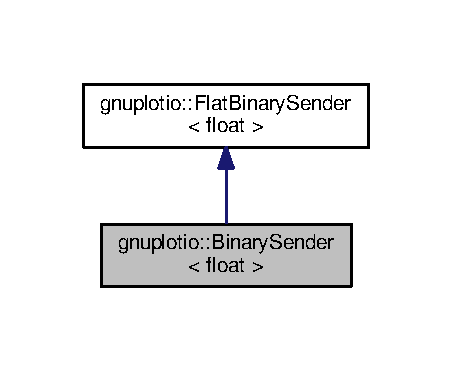
\includegraphics[width=217pt]{structgnuplotio_1_1_binary_sender_3_01float_01_4__inherit__graph}
\end{center}
\end{figure}


Collaboration diagram for gnuplotio\+:\+:Binary\+Sender$<$ float $>$\+:
\nopagebreak
\begin{figure}[H]
\begin{center}
\leavevmode
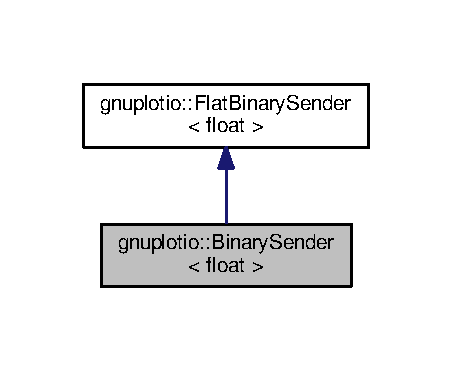
\includegraphics[width=217pt]{structgnuplotio_1_1_binary_sender_3_01float_01_4__coll__graph}
\end{center}
\end{figure}
\subsection*{Additional Inherited Members}


The documentation for this struct was generated from the following file\+:\begin{DoxyCompactItemize}
\item 
/home/rajshinde/\+G\+M\+O\+C\+K/\+Robot\+\_\+\+Controller\+\_\+\+Module/include/gnuplot-\/iostream.\+h\end{DoxyCompactItemize}

\hypertarget{structgnuplotio_1_1_binary_sender_3_01std_1_1complex_3_01_t_01_4_01_4}{}\section{gnuplotio\+:\+:Binary\+Sender$<$ std\+:\+:complex$<$ T $>$ $>$ Struct Template Reference}
\label{structgnuplotio_1_1_binary_sender_3_01std_1_1complex_3_01_t_01_4_01_4}\index{gnuplotio\+::\+Binary\+Sender$<$ std\+::complex$<$ T $>$ $>$@{gnuplotio\+::\+Binary\+Sender$<$ std\+::complex$<$ T $>$ $>$}}
\subsection*{Static Public Member Functions}
\begin{DoxyCompactItemize}
\item 
static void {\bfseries send} (std\+::ostream \&stream, const std\+::complex$<$ T $>$ \&v)\hypertarget{structgnuplotio_1_1_binary_sender_3_01std_1_1complex_3_01_t_01_4_01_4_a759de700a1cd68000830a4b15a6fec49}{}\label{structgnuplotio_1_1_binary_sender_3_01std_1_1complex_3_01_t_01_4_01_4_a759de700a1cd68000830a4b15a6fec49}

\end{DoxyCompactItemize}


The documentation for this struct was generated from the following file\+:\begin{DoxyCompactItemize}
\item 
/home/rajshinde/\+G\+M\+O\+C\+K/\+Robot\+\_\+\+Controller\+\_\+\+Module/include/gnuplot-\/iostream.\+h\end{DoxyCompactItemize}

\hypertarget{structgnuplotio_1_1_binary_sender_3_01std_1_1pair_3_01_t_00_01_u_01_4_01_4}{}\section{gnuplotio\+:\+:Binary\+Sender$<$ std\+:\+:pair$<$ T, U $>$ $>$ Struct Template Reference}
\label{structgnuplotio_1_1_binary_sender_3_01std_1_1pair_3_01_t_00_01_u_01_4_01_4}\index{gnuplotio\+::\+Binary\+Sender$<$ std\+::pair$<$ T, U $>$ $>$@{gnuplotio\+::\+Binary\+Sender$<$ std\+::pair$<$ T, U $>$ $>$}}
\subsection*{Static Public Member Functions}
\begin{DoxyCompactItemize}
\item 
static void {\bfseries send} (std\+::ostream \&stream, const std\+::pair$<$ T, U $>$ \&v)\hypertarget{structgnuplotio_1_1_binary_sender_3_01std_1_1pair_3_01_t_00_01_u_01_4_01_4_a9d949c8e7b1dea493288b0a2dd95cbff}{}\label{structgnuplotio_1_1_binary_sender_3_01std_1_1pair_3_01_t_00_01_u_01_4_01_4_a9d949c8e7b1dea493288b0a2dd95cbff}

\end{DoxyCompactItemize}


The documentation for this struct was generated from the following file\+:\begin{DoxyCompactItemize}
\item 
/home/rajshinde/\+G\+M\+O\+C\+K/\+Robot\+\_\+\+Controller\+\_\+\+Module/include/gnuplot-\/iostream.\+h\end{DoxyCompactItemize}

\hypertarget{structgnuplotio_1_1_binary_sender_3_01_t_00_01typename_01boost_1_1enable__if_3_01boost_1_1mpl_1_916ff7a758aa0b8917fd3b30ff275f06}{}\section{gnuplotio\+:\+:Binary\+Sender$<$ T, typename boost\+:\+:enable\+\_\+if$<$ boost\+:\+:mpl\+:\+:and\+\_\+$<$ is\+\_\+boost\+\_\+tuple$<$ T $>$, boost\+:\+:mpl\+:\+:not\+\_\+$<$ is\+\_\+boost\+\_\+tuple\+\_\+nulltype$<$ typename T\+:\+:tail\+\_\+type $>$ $>$ $>$ $>$\+:\+:type $>$ Struct Template Reference}
\label{structgnuplotio_1_1_binary_sender_3_01_t_00_01typename_01boost_1_1enable__if_3_01boost_1_1mpl_1_916ff7a758aa0b8917fd3b30ff275f06}\index{gnuplotio\+::\+Binary\+Sender$<$ T, typename boost\+::enable\+\_\+if$<$ boost\+::mpl\+::and\+\_\+$<$ is\+\_\+boost\+\_\+tuple$<$ T $>$, boost\+::mpl\+::not\+\_\+$<$ is\+\_\+boost\+\_\+tuple\+\_\+nulltype$<$ typename T\+::tail\+\_\+type $>$ $>$ $>$ $>$\+::type $>$@{gnuplotio\+::\+Binary\+Sender$<$ T, typename boost\+::enable\+\_\+if$<$ boost\+::mpl\+::and\+\_\+$<$ is\+\_\+boost\+\_\+tuple$<$ T $>$, boost\+::mpl\+::not\+\_\+$<$ is\+\_\+boost\+\_\+tuple\+\_\+nulltype$<$ typename T\+::tail\+\_\+type $>$ $>$ $>$ $>$\+::type $>$}}
\subsection*{Static Public Member Functions}
\begin{DoxyCompactItemize}
\item 
static void {\bfseries send} (std\+::ostream \&stream, const T \&v)\hypertarget{structgnuplotio_1_1_binary_sender_3_01_t_00_01typename_01boost_1_1enable__if_3_01boost_1_1mpl_1_916ff7a758aa0b8917fd3b30ff275f06_a90bdbe9d299646a871882da19fdb30a9}{}\label{structgnuplotio_1_1_binary_sender_3_01_t_00_01typename_01boost_1_1enable__if_3_01boost_1_1mpl_1_916ff7a758aa0b8917fd3b30ff275f06_a90bdbe9d299646a871882da19fdb30a9}

\end{DoxyCompactItemize}


The documentation for this struct was generated from the following file\+:\begin{DoxyCompactItemize}
\item 
/home/rajshinde/\+G\+M\+O\+C\+K/\+Robot\+\_\+\+Controller\+\_\+\+Module/include/gnuplot-\/iostream.\+h\end{DoxyCompactItemize}

\hypertarget{structgnuplotio_1_1_binary_sender_3_01_t_00_01typename_01boost_1_1enable__if_3_01boost_1_1mpl_1_29e1098ca8b7afc20f2ca0bc2e79506a}{}\section{gnuplotio\+:\+:Binary\+Sender$<$ T, typename boost\+:\+:enable\+\_\+if$<$ boost\+:\+:mpl\+:\+:and\+\_\+$<$ is\+\_\+boost\+\_\+tuple$<$ T $>$, is\+\_\+boost\+\_\+tuple\+\_\+nulltype$<$ typename T\+:\+:tail\+\_\+type $>$ $>$ $>$\+:\+:type $>$ Struct Template Reference}
\label{structgnuplotio_1_1_binary_sender_3_01_t_00_01typename_01boost_1_1enable__if_3_01boost_1_1mpl_1_29e1098ca8b7afc20f2ca0bc2e79506a}\index{gnuplotio\+::\+Binary\+Sender$<$ T, typename boost\+::enable\+\_\+if$<$ boost\+::mpl\+::and\+\_\+$<$ is\+\_\+boost\+\_\+tuple$<$ T $>$, is\+\_\+boost\+\_\+tuple\+\_\+nulltype$<$ typename T\+::tail\+\_\+type $>$ $>$ $>$\+::type $>$@{gnuplotio\+::\+Binary\+Sender$<$ T, typename boost\+::enable\+\_\+if$<$ boost\+::mpl\+::and\+\_\+$<$ is\+\_\+boost\+\_\+tuple$<$ T $>$, is\+\_\+boost\+\_\+tuple\+\_\+nulltype$<$ typename T\+::tail\+\_\+type $>$ $>$ $>$\+::type $>$}}
\subsection*{Static Public Member Functions}
\begin{DoxyCompactItemize}
\item 
static void {\bfseries send} (std\+::ostream \&stream, const T \&v)\hypertarget{structgnuplotio_1_1_binary_sender_3_01_t_00_01typename_01boost_1_1enable__if_3_01boost_1_1mpl_1_29e1098ca8b7afc20f2ca0bc2e79506a_a50e54b7f2aba37f1f9e63fa81941b6d6}{}\label{structgnuplotio_1_1_binary_sender_3_01_t_00_01typename_01boost_1_1enable__if_3_01boost_1_1mpl_1_29e1098ca8b7afc20f2ca0bc2e79506a_a50e54b7f2aba37f1f9e63fa81941b6d6}

\end{DoxyCompactItemize}


The documentation for this struct was generated from the following file\+:\begin{DoxyCompactItemize}
\item 
/home/rajshinde/\+G\+M\+O\+C\+K/\+Robot\+\_\+\+Controller\+\_\+\+Module/include/gnuplot-\/iostream.\+h\end{DoxyCompactItemize}

\hypertarget{structgnuplotio_1_1_binfmt_sender}{}\section{gnuplotio\+:\+:Binfmt\+Sender$<$ T, Enable $>$ Struct Template Reference}
\label{structgnuplotio_1_1_binfmt_sender}\index{gnuplotio\+::\+Binfmt\+Sender$<$ T, Enable $>$@{gnuplotio\+::\+Binfmt\+Sender$<$ T, Enable $>$}}
\subsection*{Public Member Functions}
\begin{DoxyCompactItemize}
\item 
{\bfseries G\+N\+U\+P\+L\+O\+T\+\_\+\+S\+T\+A\+T\+I\+C\+\_\+\+A\+S\+S\+E\+R\+T\+\_\+\+M\+SG} ((sizeof(T)==0),\char`\"{}Binfmt\+Sender class not specialized for this type\char`\"{})\hypertarget{structgnuplotio_1_1_binfmt_sender_ab0b554a2e81309917b2fa6f480e2a8e2}{}\label{structgnuplotio_1_1_binfmt_sender_ab0b554a2e81309917b2fa6f480e2a8e2}

\end{DoxyCompactItemize}
\subsection*{Static Public Member Functions}
\begin{DoxyCompactItemize}
\item 
static void {\bfseries send} (std\+::ostream \&)\hypertarget{structgnuplotio_1_1_binfmt_sender_a762010e3172c02e981252f93185b29c8}{}\label{structgnuplotio_1_1_binfmt_sender_a762010e3172c02e981252f93185b29c8}

\end{DoxyCompactItemize}


The documentation for this struct was generated from the following file\+:\begin{DoxyCompactItemize}
\item 
/home/rajshinde/\+G\+M\+O\+C\+K/\+Robot\+\_\+\+Controller\+\_\+\+Module/include/gnuplot-\/iostream.\+h\end{DoxyCompactItemize}

\hypertarget{structgnuplotio_1_1_binfmt_sender_3_01boost_1_1int16__t_01_4}{}\section{gnuplotio\+:\+:Binfmt\+Sender$<$ boost\+:\+:int16\+\_\+t $>$ Struct Template Reference}
\label{structgnuplotio_1_1_binfmt_sender_3_01boost_1_1int16__t_01_4}\index{gnuplotio\+::\+Binfmt\+Sender$<$ boost\+::int16\+\_\+t $>$@{gnuplotio\+::\+Binfmt\+Sender$<$ boost\+::int16\+\_\+t $>$}}
\subsection*{Static Public Member Functions}
\begin{DoxyCompactItemize}
\item 
static void {\bfseries send} (std\+::ostream \&stream)\hypertarget{structgnuplotio_1_1_binfmt_sender_3_01boost_1_1int16__t_01_4_a6d3c1b829c9196fa9d1f53bd78a90e34}{}\label{structgnuplotio_1_1_binfmt_sender_3_01boost_1_1int16__t_01_4_a6d3c1b829c9196fa9d1f53bd78a90e34}

\end{DoxyCompactItemize}


The documentation for this struct was generated from the following file\+:\begin{DoxyCompactItemize}
\item 
/home/rajshinde/\+G\+M\+O\+C\+K/\+Robot\+\_\+\+Controller\+\_\+\+Module/include/gnuplot-\/iostream.\+h\end{DoxyCompactItemize}

\hypertarget{structgnuplotio_1_1_binfmt_sender_3_01boost_1_1int32__t_01_4}{}\section{gnuplotio\+:\+:Binfmt\+Sender$<$ boost\+:\+:int32\+\_\+t $>$ Struct Template Reference}
\label{structgnuplotio_1_1_binfmt_sender_3_01boost_1_1int32__t_01_4}\index{gnuplotio\+::\+Binfmt\+Sender$<$ boost\+::int32\+\_\+t $>$@{gnuplotio\+::\+Binfmt\+Sender$<$ boost\+::int32\+\_\+t $>$}}
\subsection*{Static Public Member Functions}
\begin{DoxyCompactItemize}
\item 
static void {\bfseries send} (std\+::ostream \&stream)\hypertarget{structgnuplotio_1_1_binfmt_sender_3_01boost_1_1int32__t_01_4_a44f75b80ef3f5def62eaa2093810fd35}{}\label{structgnuplotio_1_1_binfmt_sender_3_01boost_1_1int32__t_01_4_a44f75b80ef3f5def62eaa2093810fd35}

\end{DoxyCompactItemize}


The documentation for this struct was generated from the following file\+:\begin{DoxyCompactItemize}
\item 
/home/rajshinde/\+G\+M\+O\+C\+K/\+Robot\+\_\+\+Controller\+\_\+\+Module/include/gnuplot-\/iostream.\+h\end{DoxyCompactItemize}

\hypertarget{structgnuplotio_1_1_binfmt_sender_3_01boost_1_1int64__t_01_4}{}\section{gnuplotio\+:\+:Binfmt\+Sender$<$ boost\+:\+:int64\+\_\+t $>$ Struct Template Reference}
\label{structgnuplotio_1_1_binfmt_sender_3_01boost_1_1int64__t_01_4}\index{gnuplotio\+::\+Binfmt\+Sender$<$ boost\+::int64\+\_\+t $>$@{gnuplotio\+::\+Binfmt\+Sender$<$ boost\+::int64\+\_\+t $>$}}
\subsection*{Static Public Member Functions}
\begin{DoxyCompactItemize}
\item 
static void {\bfseries send} (std\+::ostream \&stream)\hypertarget{structgnuplotio_1_1_binfmt_sender_3_01boost_1_1int64__t_01_4_a57423f02a4526e15d7d821606b1c8c81}{}\label{structgnuplotio_1_1_binfmt_sender_3_01boost_1_1int64__t_01_4_a57423f02a4526e15d7d821606b1c8c81}

\end{DoxyCompactItemize}


The documentation for this struct was generated from the following file\+:\begin{DoxyCompactItemize}
\item 
/home/rajshinde/\+G\+M\+O\+C\+K/\+Robot\+\_\+\+Controller\+\_\+\+Module/include/gnuplot-\/iostream.\+h\end{DoxyCompactItemize}

\hypertarget{structgnuplotio_1_1_binfmt_sender_3_01boost_1_1int8__t_01_4}{}\section{gnuplotio\+:\+:Binfmt\+Sender$<$ boost\+:\+:int8\+\_\+t $>$ Struct Template Reference}
\label{structgnuplotio_1_1_binfmt_sender_3_01boost_1_1int8__t_01_4}\index{gnuplotio\+::\+Binfmt\+Sender$<$ boost\+::int8\+\_\+t $>$@{gnuplotio\+::\+Binfmt\+Sender$<$ boost\+::int8\+\_\+t $>$}}
\subsection*{Static Public Member Functions}
\begin{DoxyCompactItemize}
\item 
static void {\bfseries send} (std\+::ostream \&stream)\hypertarget{structgnuplotio_1_1_binfmt_sender_3_01boost_1_1int8__t_01_4_a6f61d43b0da25f044bfad0d45fe888b4}{}\label{structgnuplotio_1_1_binfmt_sender_3_01boost_1_1int8__t_01_4_a6f61d43b0da25f044bfad0d45fe888b4}

\end{DoxyCompactItemize}


The documentation for this struct was generated from the following file\+:\begin{DoxyCompactItemize}
\item 
/home/rajshinde/\+G\+M\+O\+C\+K/\+Robot\+\_\+\+Controller\+\_\+\+Module/include/gnuplot-\/iostream.\+h\end{DoxyCompactItemize}

\hypertarget{structgnuplotio_1_1_binfmt_sender_3_01boost_1_1uint16__t_01_4}{}\section{gnuplotio\+:\+:Binfmt\+Sender$<$ boost\+:\+:uint16\+\_\+t $>$ Struct Template Reference}
\label{structgnuplotio_1_1_binfmt_sender_3_01boost_1_1uint16__t_01_4}\index{gnuplotio\+::\+Binfmt\+Sender$<$ boost\+::uint16\+\_\+t $>$@{gnuplotio\+::\+Binfmt\+Sender$<$ boost\+::uint16\+\_\+t $>$}}
\subsection*{Static Public Member Functions}
\begin{DoxyCompactItemize}
\item 
static void {\bfseries send} (std\+::ostream \&stream)\hypertarget{structgnuplotio_1_1_binfmt_sender_3_01boost_1_1uint16__t_01_4_a7bb7f0a62a21496b9e85ce35f0170717}{}\label{structgnuplotio_1_1_binfmt_sender_3_01boost_1_1uint16__t_01_4_a7bb7f0a62a21496b9e85ce35f0170717}

\end{DoxyCompactItemize}


The documentation for this struct was generated from the following file\+:\begin{DoxyCompactItemize}
\item 
/home/rajshinde/\+G\+M\+O\+C\+K/\+Robot\+\_\+\+Controller\+\_\+\+Module/include/gnuplot-\/iostream.\+h\end{DoxyCompactItemize}

\hypertarget{structgnuplotio_1_1_binfmt_sender_3_01boost_1_1uint32__t_01_4}{}\section{gnuplotio\+:\+:Binfmt\+Sender$<$ boost\+:\+:uint32\+\_\+t $>$ Struct Template Reference}
\label{structgnuplotio_1_1_binfmt_sender_3_01boost_1_1uint32__t_01_4}\index{gnuplotio\+::\+Binfmt\+Sender$<$ boost\+::uint32\+\_\+t $>$@{gnuplotio\+::\+Binfmt\+Sender$<$ boost\+::uint32\+\_\+t $>$}}
\subsection*{Static Public Member Functions}
\begin{DoxyCompactItemize}
\item 
static void {\bfseries send} (std\+::ostream \&stream)\hypertarget{structgnuplotio_1_1_binfmt_sender_3_01boost_1_1uint32__t_01_4_a134bce57dc5bb3e06c1b369a9826403b}{}\label{structgnuplotio_1_1_binfmt_sender_3_01boost_1_1uint32__t_01_4_a134bce57dc5bb3e06c1b369a9826403b}

\end{DoxyCompactItemize}


The documentation for this struct was generated from the following file\+:\begin{DoxyCompactItemize}
\item 
/home/rajshinde/\+G\+M\+O\+C\+K/\+Robot\+\_\+\+Controller\+\_\+\+Module/include/gnuplot-\/iostream.\+h\end{DoxyCompactItemize}

\hypertarget{structgnuplotio_1_1_binfmt_sender_3_01boost_1_1uint64__t_01_4}{}\section{gnuplotio\+:\+:Binfmt\+Sender$<$ boost\+:\+:uint64\+\_\+t $>$ Struct Template Reference}
\label{structgnuplotio_1_1_binfmt_sender_3_01boost_1_1uint64__t_01_4}\index{gnuplotio\+::\+Binfmt\+Sender$<$ boost\+::uint64\+\_\+t $>$@{gnuplotio\+::\+Binfmt\+Sender$<$ boost\+::uint64\+\_\+t $>$}}
\subsection*{Static Public Member Functions}
\begin{DoxyCompactItemize}
\item 
static void {\bfseries send} (std\+::ostream \&stream)\hypertarget{structgnuplotio_1_1_binfmt_sender_3_01boost_1_1uint64__t_01_4_a9f57162a6baf940675236235556f62ba}{}\label{structgnuplotio_1_1_binfmt_sender_3_01boost_1_1uint64__t_01_4_a9f57162a6baf940675236235556f62ba}

\end{DoxyCompactItemize}


The documentation for this struct was generated from the following file\+:\begin{DoxyCompactItemize}
\item 
/home/rajshinde/\+G\+M\+O\+C\+K/\+Robot\+\_\+\+Controller\+\_\+\+Module/include/gnuplot-\/iostream.\+h\end{DoxyCompactItemize}

\hypertarget{structgnuplotio_1_1_binfmt_sender_3_01boost_1_1uint8__t_01_4}{}\section{gnuplotio\+:\+:Binfmt\+Sender$<$ boost\+:\+:uint8\+\_\+t $>$ Struct Template Reference}
\label{structgnuplotio_1_1_binfmt_sender_3_01boost_1_1uint8__t_01_4}\index{gnuplotio\+::\+Binfmt\+Sender$<$ boost\+::uint8\+\_\+t $>$@{gnuplotio\+::\+Binfmt\+Sender$<$ boost\+::uint8\+\_\+t $>$}}
\subsection*{Static Public Member Functions}
\begin{DoxyCompactItemize}
\item 
static void {\bfseries send} (std\+::ostream \&stream)\hypertarget{structgnuplotio_1_1_binfmt_sender_3_01boost_1_1uint8__t_01_4_a57d45c45f1ee19614c972bc82c4b214c}{}\label{structgnuplotio_1_1_binfmt_sender_3_01boost_1_1uint8__t_01_4_a57d45c45f1ee19614c972bc82c4b214c}

\end{DoxyCompactItemize}


The documentation for this struct was generated from the following file\+:\begin{DoxyCompactItemize}
\item 
/home/rajshinde/\+G\+M\+O\+C\+K/\+Robot\+\_\+\+Controller\+\_\+\+Module/include/gnuplot-\/iostream.\+h\end{DoxyCompactItemize}

\hypertarget{structgnuplotio_1_1_binfmt_sender_3_01double_01_4}{}\section{gnuplotio\+:\+:Binfmt\+Sender$<$ double $>$ Struct Template Reference}
\label{structgnuplotio_1_1_binfmt_sender_3_01double_01_4}\index{gnuplotio\+::\+Binfmt\+Sender$<$ double $>$@{gnuplotio\+::\+Binfmt\+Sender$<$ double $>$}}
\subsection*{Static Public Member Functions}
\begin{DoxyCompactItemize}
\item 
static void {\bfseries send} (std\+::ostream \&stream)\hypertarget{structgnuplotio_1_1_binfmt_sender_3_01double_01_4_a455b75492a6a86398374d14a2bfc7238}{}\label{structgnuplotio_1_1_binfmt_sender_3_01double_01_4_a455b75492a6a86398374d14a2bfc7238}

\end{DoxyCompactItemize}


The documentation for this struct was generated from the following file\+:\begin{DoxyCompactItemize}
\item 
/home/rajshinde/\+G\+M\+O\+C\+K/\+Robot\+\_\+\+Controller\+\_\+\+Module/include/gnuplot-\/iostream.\+h\end{DoxyCompactItemize}

\hypertarget{structgnuplotio_1_1_binfmt_sender_3_01float_01_4}{}\section{gnuplotio\+:\+:Binfmt\+Sender$<$ float $>$ Struct Template Reference}
\label{structgnuplotio_1_1_binfmt_sender_3_01float_01_4}\index{gnuplotio\+::\+Binfmt\+Sender$<$ float $>$@{gnuplotio\+::\+Binfmt\+Sender$<$ float $>$}}
\subsection*{Static Public Member Functions}
\begin{DoxyCompactItemize}
\item 
static void {\bfseries send} (std\+::ostream \&stream)\hypertarget{structgnuplotio_1_1_binfmt_sender_3_01float_01_4_ae9c6a1915ee24e54ea5ed1a22c54fee1}{}\label{structgnuplotio_1_1_binfmt_sender_3_01float_01_4_ae9c6a1915ee24e54ea5ed1a22c54fee1}

\end{DoxyCompactItemize}


The documentation for this struct was generated from the following file\+:\begin{DoxyCompactItemize}
\item 
/home/rajshinde/\+G\+M\+O\+C\+K/\+Robot\+\_\+\+Controller\+\_\+\+Module/include/gnuplot-\/iostream.\+h\end{DoxyCompactItemize}

\hypertarget{structgnuplotio_1_1_binfmt_sender_3_01std_1_1complex_3_01_t_01_4_01_4}{}\section{gnuplotio\+:\+:Binfmt\+Sender$<$ std\+:\+:complex$<$ T $>$ $>$ Struct Template Reference}
\label{structgnuplotio_1_1_binfmt_sender_3_01std_1_1complex_3_01_t_01_4_01_4}\index{gnuplotio\+::\+Binfmt\+Sender$<$ std\+::complex$<$ T $>$ $>$@{gnuplotio\+::\+Binfmt\+Sender$<$ std\+::complex$<$ T $>$ $>$}}
\subsection*{Static Public Member Functions}
\begin{DoxyCompactItemize}
\item 
static void {\bfseries send} (std\+::ostream \&stream)\hypertarget{structgnuplotio_1_1_binfmt_sender_3_01std_1_1complex_3_01_t_01_4_01_4_a64633d068c93ef2822ee3aa6ef39d623}{}\label{structgnuplotio_1_1_binfmt_sender_3_01std_1_1complex_3_01_t_01_4_01_4_a64633d068c93ef2822ee3aa6ef39d623}

\end{DoxyCompactItemize}


The documentation for this struct was generated from the following file\+:\begin{DoxyCompactItemize}
\item 
/home/rajshinde/\+G\+M\+O\+C\+K/\+Robot\+\_\+\+Controller\+\_\+\+Module/include/gnuplot-\/iostream.\+h\end{DoxyCompactItemize}

\hypertarget{structgnuplotio_1_1_binfmt_sender_3_01std_1_1pair_3_01_t_00_01_u_01_4_01_4}{}\section{gnuplotio\+:\+:Binfmt\+Sender$<$ std\+:\+:pair$<$ T, U $>$ $>$ Struct Template Reference}
\label{structgnuplotio_1_1_binfmt_sender_3_01std_1_1pair_3_01_t_00_01_u_01_4_01_4}\index{gnuplotio\+::\+Binfmt\+Sender$<$ std\+::pair$<$ T, U $>$ $>$@{gnuplotio\+::\+Binfmt\+Sender$<$ std\+::pair$<$ T, U $>$ $>$}}
\subsection*{Static Public Member Functions}
\begin{DoxyCompactItemize}
\item 
static void {\bfseries send} (std\+::ostream \&stream)\hypertarget{structgnuplotio_1_1_binfmt_sender_3_01std_1_1pair_3_01_t_00_01_u_01_4_01_4_a08b2bedbc54824cd202c664116e37243}{}\label{structgnuplotio_1_1_binfmt_sender_3_01std_1_1pair_3_01_t_00_01_u_01_4_01_4_a08b2bedbc54824cd202c664116e37243}

\end{DoxyCompactItemize}


The documentation for this struct was generated from the following file\+:\begin{DoxyCompactItemize}
\item 
/home/rajshinde/\+G\+M\+O\+C\+K/\+Robot\+\_\+\+Controller\+\_\+\+Module/include/gnuplot-\/iostream.\+h\end{DoxyCompactItemize}

\hypertarget{structgnuplotio_1_1_binfmt_sender_3_01_t_00_01typename_01boost_1_1enable__if_3_01boost_1_1mpl_1_e9270e5cb86823566a0af3940aa51061}{}\section{gnuplotio\+:\+:Binfmt\+Sender$<$ T, typename boost\+:\+:enable\+\_\+if$<$ boost\+:\+:mpl\+:\+:and\+\_\+$<$ is\+\_\+boost\+\_\+tuple$<$ T $>$, boost\+:\+:mpl\+:\+:not\+\_\+$<$ is\+\_\+boost\+\_\+tuple\+\_\+nulltype$<$ typename T\+:\+:tail\+\_\+type $>$ $>$ $>$ $>$\+:\+:type $>$ Struct Template Reference}
\label{structgnuplotio_1_1_binfmt_sender_3_01_t_00_01typename_01boost_1_1enable__if_3_01boost_1_1mpl_1_e9270e5cb86823566a0af3940aa51061}\index{gnuplotio\+::\+Binfmt\+Sender$<$ T, typename boost\+::enable\+\_\+if$<$ boost\+::mpl\+::and\+\_\+$<$ is\+\_\+boost\+\_\+tuple$<$ T $>$, boost\+::mpl\+::not\+\_\+$<$ is\+\_\+boost\+\_\+tuple\+\_\+nulltype$<$ typename T\+::tail\+\_\+type $>$ $>$ $>$ $>$\+::type $>$@{gnuplotio\+::\+Binfmt\+Sender$<$ T, typename boost\+::enable\+\_\+if$<$ boost\+::mpl\+::and\+\_\+$<$ is\+\_\+boost\+\_\+tuple$<$ T $>$, boost\+::mpl\+::not\+\_\+$<$ is\+\_\+boost\+\_\+tuple\+\_\+nulltype$<$ typename T\+::tail\+\_\+type $>$ $>$ $>$ $>$\+::type $>$}}
\subsection*{Static Public Member Functions}
\begin{DoxyCompactItemize}
\item 
static void {\bfseries send} (std\+::ostream \&stream)\hypertarget{structgnuplotio_1_1_binfmt_sender_3_01_t_00_01typename_01boost_1_1enable__if_3_01boost_1_1mpl_1_e9270e5cb86823566a0af3940aa51061_a12e1b40a6ae29940661b7609df3c40ba}{}\label{structgnuplotio_1_1_binfmt_sender_3_01_t_00_01typename_01boost_1_1enable__if_3_01boost_1_1mpl_1_e9270e5cb86823566a0af3940aa51061_a12e1b40a6ae29940661b7609df3c40ba}

\end{DoxyCompactItemize}


The documentation for this struct was generated from the following file\+:\begin{DoxyCompactItemize}
\item 
/home/rajshinde/\+G\+M\+O\+C\+K/\+Robot\+\_\+\+Controller\+\_\+\+Module/include/gnuplot-\/iostream.\+h\end{DoxyCompactItemize}

\hypertarget{structgnuplotio_1_1_binfmt_sender_3_01_t_00_01typename_01boost_1_1enable__if_3_01boost_1_1mpl_1_8c86f170c2e2969f5519817e5c367132}{}\section{gnuplotio\+:\+:Binfmt\+Sender$<$ T, typename boost\+:\+:enable\+\_\+if$<$ boost\+:\+:mpl\+:\+:and\+\_\+$<$ is\+\_\+boost\+\_\+tuple$<$ T $>$, is\+\_\+boost\+\_\+tuple\+\_\+nulltype$<$ typename T\+:\+:tail\+\_\+type $>$ $>$ $>$\+:\+:type $>$ Struct Template Reference}
\label{structgnuplotio_1_1_binfmt_sender_3_01_t_00_01typename_01boost_1_1enable__if_3_01boost_1_1mpl_1_8c86f170c2e2969f5519817e5c367132}\index{gnuplotio\+::\+Binfmt\+Sender$<$ T, typename boost\+::enable\+\_\+if$<$ boost\+::mpl\+::and\+\_\+$<$ is\+\_\+boost\+\_\+tuple$<$ T $>$, is\+\_\+boost\+\_\+tuple\+\_\+nulltype$<$ typename T\+::tail\+\_\+type $>$ $>$ $>$\+::type $>$@{gnuplotio\+::\+Binfmt\+Sender$<$ T, typename boost\+::enable\+\_\+if$<$ boost\+::mpl\+::and\+\_\+$<$ is\+\_\+boost\+\_\+tuple$<$ T $>$, is\+\_\+boost\+\_\+tuple\+\_\+nulltype$<$ typename T\+::tail\+\_\+type $>$ $>$ $>$\+::type $>$}}
\subsection*{Static Public Member Functions}
\begin{DoxyCompactItemize}
\item 
static void {\bfseries send} (std\+::ostream \&stream)\hypertarget{structgnuplotio_1_1_binfmt_sender_3_01_t_00_01typename_01boost_1_1enable__if_3_01boost_1_1mpl_1_8c86f170c2e2969f5519817e5c367132_aa1850ae529cdb36fedc67c5ebfa3f871}{}\label{structgnuplotio_1_1_binfmt_sender_3_01_t_00_01typename_01boost_1_1enable__if_3_01boost_1_1mpl_1_8c86f170c2e2969f5519817e5c367132_aa1850ae529cdb36fedc67c5ebfa3f871}

\end{DoxyCompactItemize}


The documentation for this struct was generated from the following file\+:\begin{DoxyCompactItemize}
\item 
/home/rajshinde/\+G\+M\+O\+C\+K/\+Robot\+\_\+\+Controller\+\_\+\+Module/include/gnuplot-\/iostream.\+h\end{DoxyCompactItemize}

\hypertarget{structgnuplotio_1_1_cast_int_text_sender}{}\section{gnuplotio\+:\+:Cast\+Int\+Text\+Sender$<$ T $>$ Struct Template Reference}
\label{structgnuplotio_1_1_cast_int_text_sender}\index{gnuplotio\+::\+Cast\+Int\+Text\+Sender$<$ T $>$@{gnuplotio\+::\+Cast\+Int\+Text\+Sender$<$ T $>$}}
\subsection*{Static Public Member Functions}
\begin{DoxyCompactItemize}
\item 
static void {\bfseries send} (std\+::ostream \&stream, const T \&v)\hypertarget{structgnuplotio_1_1_cast_int_text_sender_a42733f83f843a375437e7e5f716ea65e}{}\label{structgnuplotio_1_1_cast_int_text_sender_a42733f83f843a375437e7e5f716ea65e}

\end{DoxyCompactItemize}


The documentation for this struct was generated from the following file\+:\begin{DoxyCompactItemize}
\item 
/home/rajshinde/\+G\+M\+O\+C\+K/\+Robot\+\_\+\+Controller\+\_\+\+Module/include/gnuplot-\/iostream.\+h\end{DoxyCompactItemize}

\hypertarget{structgnuplotio_1_1_col_unwrap_no}{}\section{gnuplotio\+:\+:Col\+Unwrap\+No Struct Reference}
\label{structgnuplotio_1_1_col_unwrap_no}\index{gnuplotio\+::\+Col\+Unwrap\+No@{gnuplotio\+::\+Col\+Unwrap\+No}}


The documentation for this struct was generated from the following file\+:\begin{DoxyCompactItemize}
\item 
/home/rajshinde/\+G\+M\+O\+C\+K/\+Robot\+\_\+\+Controller\+\_\+\+Module/include/gnuplot-\/iostream.\+h\end{DoxyCompactItemize}

\hypertarget{structgnuplotio_1_1_col_unwrap_yes}{}\section{gnuplotio\+:\+:Col\+Unwrap\+Yes Struct Reference}
\label{structgnuplotio_1_1_col_unwrap_yes}\index{gnuplotio\+::\+Col\+Unwrap\+Yes@{gnuplotio\+::\+Col\+Unwrap\+Yes}}


The documentation for this struct was generated from the following file\+:\begin{DoxyCompactItemize}
\item 
/home/rajshinde/\+G\+M\+O\+C\+K/\+Robot\+\_\+\+Controller\+\_\+\+Module/include/gnuplot-\/iostream.\+h\end{DoxyCompactItemize}

\hypertarget{structgnuplotio_1_1dont__treat__as__stl__container}{}\section{gnuplotio\+:\+:dont\+\_\+treat\+\_\+as\+\_\+stl\+\_\+container$<$ T $>$ Struct Template Reference}
\label{structgnuplotio_1_1dont__treat__as__stl__container}\index{gnuplotio\+::dont\+\_\+treat\+\_\+as\+\_\+stl\+\_\+container$<$ T $>$@{gnuplotio\+::dont\+\_\+treat\+\_\+as\+\_\+stl\+\_\+container$<$ T $>$}}
\subsection*{Public Types}
\begin{DoxyCompactItemize}
\item 
typedef boost\+::mpl\+::bool\+\_\+$<$ false $>$ {\bfseries type}\hypertarget{structgnuplotio_1_1dont__treat__as__stl__container_aa4404164a7547142376a9140ef07fd2a}{}\label{structgnuplotio_1_1dont__treat__as__stl__container_aa4404164a7547142376a9140ef07fd2a}

\end{DoxyCompactItemize}


The documentation for this struct was generated from the following file\+:\begin{DoxyCompactItemize}
\item 
/home/rajshinde/\+G\+M\+O\+C\+K/\+Robot\+\_\+\+Controller\+\_\+\+Module/include/gnuplot-\/iostream.\+h\end{DoxyCompactItemize}

\hypertarget{structgnuplotio_1_1_error___inappropriate_deref}{}\section{gnuplotio\+:\+:Error\+\_\+\+Inappropriate\+Deref Struct Reference}
\label{structgnuplotio_1_1_error___inappropriate_deref}\index{gnuplotio\+::\+Error\+\_\+\+Inappropriate\+Deref@{gnuplotio\+::\+Error\+\_\+\+Inappropriate\+Deref}}


The documentation for this struct was generated from the following file\+:\begin{DoxyCompactItemize}
\item 
/home/rajshinde/\+G\+M\+O\+C\+K/\+Robot\+\_\+\+Controller\+\_\+\+Module/include/gnuplot-\/iostream.\+h\end{DoxyCompactItemize}

\hypertarget{structgnuplotio_1_1_error___was_not_container}{}\section{gnuplotio\+:\+:Error\+\_\+\+Was\+Not\+Container Struct Reference}
\label{structgnuplotio_1_1_error___was_not_container}\index{gnuplotio\+::\+Error\+\_\+\+Was\+Not\+Container@{gnuplotio\+::\+Error\+\_\+\+Was\+Not\+Container}}
\subsection*{Public Types}
\begin{DoxyCompactItemize}
\item 
typedef void {\bfseries subiter\+\_\+type}\hypertarget{structgnuplotio_1_1_error___was_not_container_aeac5de90c903be765130fc14f85dfb00}{}\label{structgnuplotio_1_1_error___was_not_container_aeac5de90c903be765130fc14f85dfb00}

\end{DoxyCompactItemize}


The documentation for this struct was generated from the following file\+:\begin{DoxyCompactItemize}
\item 
/home/rajshinde/\+G\+M\+O\+C\+K/\+Robot\+\_\+\+Controller\+\_\+\+Module/include/gnuplot-\/iostream.\+h\end{DoxyCompactItemize}

\hypertarget{structgnuplotio_1_1_file_handle_wrapper}{}\section{gnuplotio\+:\+:File\+Handle\+Wrapper Struct Reference}
\label{structgnuplotio_1_1_file_handle_wrapper}\index{gnuplotio\+::\+File\+Handle\+Wrapper@{gnuplotio\+::\+File\+Handle\+Wrapper}}


Inheritance diagram for gnuplotio\+:\+:File\+Handle\+Wrapper\+:
\nopagebreak
\begin{figure}[H]
\begin{center}
\leavevmode
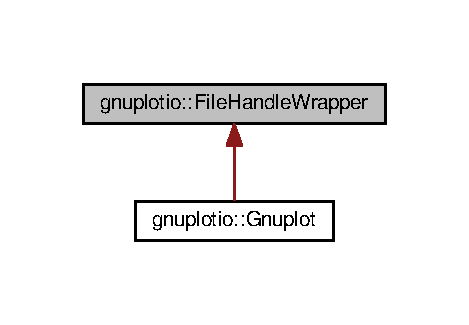
\includegraphics[width=225pt]{structgnuplotio_1_1_file_handle_wrapper__inherit__graph}
\end{center}
\end{figure}
\subsection*{Public Member Functions}
\begin{DoxyCompactItemize}
\item 
{\bfseries File\+Handle\+Wrapper} (std\+::\+F\+I\+LE $\ast$\+\_\+fh, bool \+\_\+should\+\_\+use\+\_\+pclose)\hypertarget{structgnuplotio_1_1_file_handle_wrapper_a26b2378e193a9c41be5aed97e11f9411}{}\label{structgnuplotio_1_1_file_handle_wrapper_a26b2378e193a9c41be5aed97e11f9411}

\item 
void {\bfseries fh\+\_\+close} ()\hypertarget{structgnuplotio_1_1_file_handle_wrapper_acafac45efd9c78ce621af4f3228c6f67}{}\label{structgnuplotio_1_1_file_handle_wrapper_acafac45efd9c78ce621af4f3228c6f67}

\item 
int {\bfseries fh\+\_\+fileno} ()\hypertarget{structgnuplotio_1_1_file_handle_wrapper_a3202ccd15d624f26dd2cf699d3456de6}{}\label{structgnuplotio_1_1_file_handle_wrapper_a3202ccd15d624f26dd2cf699d3456de6}

\end{DoxyCompactItemize}
\subsection*{Public Attributes}
\begin{DoxyCompactItemize}
\item 
std\+::\+F\+I\+LE $\ast$ {\bfseries wrapped\+\_\+fh}\hypertarget{structgnuplotio_1_1_file_handle_wrapper_adcb58bfcd9dbdba000a7e7395bee2ef9}{}\label{structgnuplotio_1_1_file_handle_wrapper_adcb58bfcd9dbdba000a7e7395bee2ef9}

\item 
bool {\bfseries should\+\_\+use\+\_\+pclose}\hypertarget{structgnuplotio_1_1_file_handle_wrapper_a11b63ed64cf53167e26c5273778d90ea}{}\label{structgnuplotio_1_1_file_handle_wrapper_a11b63ed64cf53167e26c5273778d90ea}

\end{DoxyCompactItemize}


The documentation for this struct was generated from the following file\+:\begin{DoxyCompactItemize}
\item 
/home/rajshinde/\+G\+M\+O\+C\+K/\+Robot\+\_\+\+Controller\+\_\+\+Module/include/gnuplot-\/iostream.\+h\end{DoxyCompactItemize}

\hypertarget{structgnuplotio_1_1_flat_binary_sender}{}\section{gnuplotio\+:\+:Flat\+Binary\+Sender$<$ T $>$ Struct Template Reference}
\label{structgnuplotio_1_1_flat_binary_sender}\index{gnuplotio\+::\+Flat\+Binary\+Sender$<$ T $>$@{gnuplotio\+::\+Flat\+Binary\+Sender$<$ T $>$}}
\subsection*{Static Public Member Functions}
\begin{DoxyCompactItemize}
\item 
static void {\bfseries send} (std\+::ostream \&stream, const T \&v)\hypertarget{structgnuplotio_1_1_flat_binary_sender_a24d085492f2539c14033cd5c6ba75ba5}{}\label{structgnuplotio_1_1_flat_binary_sender_a24d085492f2539c14033cd5c6ba75ba5}

\end{DoxyCompactItemize}


The documentation for this struct was generated from the following file\+:\begin{DoxyCompactItemize}
\item 
/home/rajshinde/\+G\+M\+O\+C\+K/\+Robot\+\_\+\+Controller\+\_\+\+Module/include/gnuplot-\/iostream.\+h\end{DoxyCompactItemize}

\hypertarget{structgnuplotio_1_1_float_text_sender}{}\section{gnuplotio\+:\+:Float\+Text\+Sender$<$ T $>$ Struct Template Reference}
\label{structgnuplotio_1_1_float_text_sender}\index{gnuplotio\+::\+Float\+Text\+Sender$<$ T $>$@{gnuplotio\+::\+Float\+Text\+Sender$<$ T $>$}}
\subsection*{Static Public Member Functions}
\begin{DoxyCompactItemize}
\item 
static void {\bfseries send} (std\+::ostream \&stream, const T \&v)\hypertarget{structgnuplotio_1_1_float_text_sender_aed6b6c3a95b1396688800d6d1f2fc299}{}\label{structgnuplotio_1_1_float_text_sender_aed6b6c3a95b1396688800d6d1f2fc299}

\end{DoxyCompactItemize}


The documentation for this struct was generated from the following file\+:\begin{DoxyCompactItemize}
\item 
/home/rajshinde/\+G\+M\+O\+C\+K/\+Robot\+\_\+\+Controller\+\_\+\+Module/include/gnuplot-\/iostream.\+h\end{DoxyCompactItemize}

\hypertarget{classgnuplotio_1_1_gnuplot}{}\section{gnuplotio\+:\+:Gnuplot Class Reference}
\label{classgnuplotio_1_1_gnuplot}\index{gnuplotio\+::\+Gnuplot@{gnuplotio\+::\+Gnuplot}}


Inheritance diagram for gnuplotio\+:\+:Gnuplot\+:
\nopagebreak
\begin{figure}[H]
\begin{center}
\leavevmode
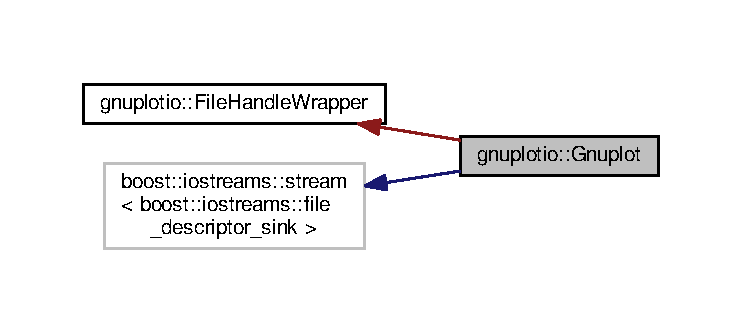
\includegraphics[width=350pt]{classgnuplotio_1_1_gnuplot__inherit__graph}
\end{center}
\end{figure}


Collaboration diagram for gnuplotio\+:\+:Gnuplot\+:
\nopagebreak
\begin{figure}[H]
\begin{center}
\leavevmode
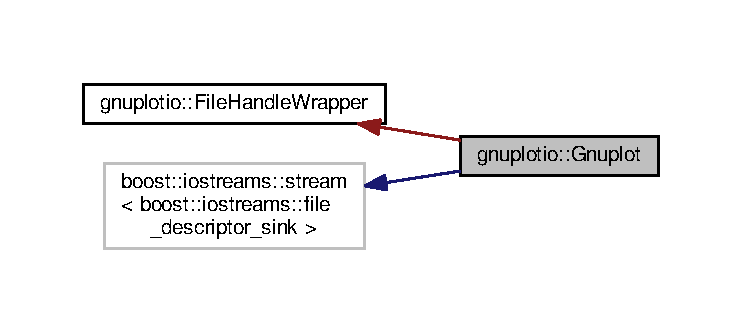
\includegraphics[width=350pt]{classgnuplotio_1_1_gnuplot__coll__graph}
\end{center}
\end{figure}
\subsection*{Public Member Functions}
\begin{DoxyCompactItemize}
\item 
{\bfseries Gnuplot} (const std\+::string \&\+\_\+cmd=\char`\"{}\char`\"{})\hypertarget{classgnuplotio_1_1_gnuplot_ab2fb14389ab63ad5d9b2e57169bbbf1d}{}\label{classgnuplotio_1_1_gnuplot_ab2fb14389ab63ad5d9b2e57169bbbf1d}

\item 
{\bfseries Gnuplot} (F\+I\+LE $\ast$\+\_\+fh)\hypertarget{classgnuplotio_1_1_gnuplot_a4a4f48a548e6ce6d485ca0a868410078}{}\label{classgnuplotio_1_1_gnuplot_a4a4f48a548e6ce6d485ca0a868410078}

\item 
void {\bfseries clear\+Tmpfiles} ()\hypertarget{classgnuplotio_1_1_gnuplot_a0d62f80988c3db4413a668e366406393}{}\label{classgnuplotio_1_1_gnuplot_a0d62f80988c3db4413a668e366406393}

\item 
{\footnotesize template$<$typename T , typename Organization\+Mode $>$ }\\\hyperlink{classgnuplotio_1_1_gnuplot}{Gnuplot} \& {\bfseries send} (const T \&arg, Organization\+Mode)\hypertarget{classgnuplotio_1_1_gnuplot_ae3f4c07960aa5601cc72158be67f945c}{}\label{classgnuplotio_1_1_gnuplot_ae3f4c07960aa5601cc72158be67f945c}

\item 
{\footnotesize template$<$typename T , typename Organization\+Mode $>$ }\\\hyperlink{classgnuplotio_1_1_gnuplot}{Gnuplot} \& {\bfseries send\+Binary} (const T \&arg, Organization\+Mode)\hypertarget{classgnuplotio_1_1_gnuplot_a46c9e01d2030768cd811d2e8dbd10dfa}{}\label{classgnuplotio_1_1_gnuplot_a46c9e01d2030768cd811d2e8dbd10dfa}

\item 
{\footnotesize template$<$typename T , typename Organization\+Mode $>$ }\\std\+::string {\bfseries binfmt} (const T \&arg, const std\+::string \&arr\+\_\+or\+\_\+rec, Organization\+Mode)\hypertarget{classgnuplotio_1_1_gnuplot_a43fe103649ec168b453c43aecdacce81}{}\label{classgnuplotio_1_1_gnuplot_a43fe103649ec168b453c43aecdacce81}

\item 
{\footnotesize template$<$typename T , typename Organization\+Mode $>$ }\\std\+::string {\bfseries file} (const T \&arg, std\+::string filename, Organization\+Mode)\hypertarget{classgnuplotio_1_1_gnuplot_a9b9980e3b3d7cbb233a989e27468fa55}{}\label{classgnuplotio_1_1_gnuplot_a9b9980e3b3d7cbb233a989e27468fa55}

\item 
{\footnotesize template$<$typename T , typename Organization\+Mode $>$ }\\std\+::string {\bfseries binary\+File} (const T \&arg, std\+::string filename, const std\+::string \&arr\+\_\+or\+\_\+rec, Organization\+Mode)\hypertarget{classgnuplotio_1_1_gnuplot_ad90501e6dbab5379abcd76fd0e2e4ef1}{}\label{classgnuplotio_1_1_gnuplot_ad90501e6dbab5379abcd76fd0e2e4ef1}

\item 
{\footnotesize template$<$typename T $>$ }\\\hyperlink{classgnuplotio_1_1_gnuplot}{Gnuplot} {\bfseries G\+N\+U\+P\+L\+O\+T\+\_\+\+D\+E\+P\+R\+E\+C\+A\+TE} (\char`\"{}use send1d or send2d\char`\"{})\&send(const T \&arg)\hypertarget{classgnuplotio_1_1_gnuplot_ab2edc3c8f57483c6d9db86d685f3eee7}{}\label{classgnuplotio_1_1_gnuplot_ab2edc3c8f57483c6d9db86d685f3eee7}

\item 
{\footnotesize template$<$typename T $>$ }\\std\+::string {\bfseries G\+N\+U\+P\+L\+O\+T\+\_\+\+D\+E\+P\+R\+E\+C\+A\+TE} (\char`\"{}use binfmt1d or binfmt2d\char`\"{}) binfmt(const T \&arg\hypertarget{classgnuplotio_1_1_gnuplot_aeb3ba94ed04ecd46b55f89591ba23e7c}{}\label{classgnuplotio_1_1_gnuplot_aeb3ba94ed04ecd46b55f89591ba23e7c}

\end{DoxyCompactItemize}
\subsection*{Public Attributes}
\begin{DoxyCompactItemize}
\item 
std\+::string const std\+::string \& {\bfseries arr\+\_\+or\+\_\+rec}\hypertarget{classgnuplotio_1_1_gnuplot_a2d194dbd4d2f3475ff6f9b8384e62a9f}{}\label{classgnuplotio_1_1_gnuplot_a2d194dbd4d2f3475ff6f9b8384e62a9f}

\item 
std\+::vector$<$ int $>$ {\bfseries tmp\+\_\+files}\hypertarget{classgnuplotio_1_1_gnuplot_a92a4f6322e486de17db4507a5fc77348}{}\label{classgnuplotio_1_1_gnuplot_a92a4f6322e486de17db4507a5fc77348}

\item 
bool {\bfseries debug\+\_\+messages}\hypertarget{classgnuplotio_1_1_gnuplot_a63e08bfd0cd02937d895ecfb6180107c}{}\label{classgnuplotio_1_1_gnuplot_a63e08bfd0cd02937d895ecfb6180107c}

\end{DoxyCompactItemize}


The documentation for this class was generated from the following file\+:\begin{DoxyCompactItemize}
\item 
/home/rajshinde/\+G\+M\+O\+C\+K/\+Robot\+\_\+\+Controller\+\_\+\+Module/include/gnuplot-\/iostream.\+h\end{DoxyCompactItemize}

\hypertarget{classgnuplotio_1_1_gnuplot_feedback}{}\section{gnuplotio\+:\+:Gnuplot\+Feedback Class Reference}
\label{classgnuplotio_1_1_gnuplot_feedback}\index{gnuplotio\+::\+Gnuplot\+Feedback@{gnuplotio\+::\+Gnuplot\+Feedback}}
\subsection*{Public Member Functions}
\begin{DoxyCompactItemize}
\item 
virtual std\+::string {\bfseries filename} () const =0\hypertarget{classgnuplotio_1_1_gnuplot_feedback_a081d4d59ffd81e2322c07c0a802e1307}{}\label{classgnuplotio_1_1_gnuplot_feedback_a081d4d59ffd81e2322c07c0a802e1307}

\item 
virtual F\+I\+LE $\ast$ {\bfseries handle} () const =0\hypertarget{classgnuplotio_1_1_gnuplot_feedback_a13ae87ba489bfbe87f64b8b54e8a4563}{}\label{classgnuplotio_1_1_gnuplot_feedback_a13ae87ba489bfbe87f64b8b54e8a4563}

\end{DoxyCompactItemize}


The documentation for this class was generated from the following file\+:\begin{DoxyCompactItemize}
\item 
/home/rajshinde/\+G\+M\+O\+C\+K/\+Robot\+\_\+\+Controller\+\_\+\+Module/include/gnuplot-\/iostream.\+h\end{DoxyCompactItemize}

\hypertarget{structgnuplotio_1_1is__boost__tuple}{}\section{gnuplotio\+:\+:is\+\_\+boost\+\_\+tuple$<$ T $>$ Struct Template Reference}
\label{structgnuplotio_1_1is__boost__tuple}\index{gnuplotio\+::is\+\_\+boost\+\_\+tuple$<$ T $>$@{gnuplotio\+::is\+\_\+boost\+\_\+tuple$<$ T $>$}}
\subsection*{Public Types}
\begin{DoxyCompactItemize}
\item 
typedef boost\+::mpl\+::and\+\_\+$<$ typename has\+\_\+head\+\_\+type$<$ T $>$\+::type, typename has\+\_\+tail\+\_\+type$<$ T $>$\+::type $>$ {\bfseries type}\hypertarget{structgnuplotio_1_1is__boost__tuple_ad771f62833b23ecae5dc689e6248396a}{}\label{structgnuplotio_1_1is__boost__tuple_ad771f62833b23ecae5dc689e6248396a}

\end{DoxyCompactItemize}
\subsection*{Static Public Attributes}
\begin{DoxyCompactItemize}
\item 
static const bool {\bfseries value} = type\+::value\hypertarget{structgnuplotio_1_1is__boost__tuple_ae6664b02421d28585204104af65a4744}{}\label{structgnuplotio_1_1is__boost__tuple_ae6664b02421d28585204104af65a4744}

\end{DoxyCompactItemize}


The documentation for this struct was generated from the following file\+:\begin{DoxyCompactItemize}
\item 
/home/rajshinde/\+G\+M\+O\+C\+K/\+Robot\+\_\+\+Controller\+\_\+\+Module/include/gnuplot-\/iostream.\+h\end{DoxyCompactItemize}

\hypertarget{structgnuplotio_1_1is__boost__tuple__nulltype}{}\section{gnuplotio\+:\+:is\+\_\+boost\+\_\+tuple\+\_\+nulltype$<$ T $>$ Struct Template Reference}
\label{structgnuplotio_1_1is__boost__tuple__nulltype}\index{gnuplotio\+::is\+\_\+boost\+\_\+tuple\+\_\+nulltype$<$ T $>$@{gnuplotio\+::is\+\_\+boost\+\_\+tuple\+\_\+nulltype$<$ T $>$}}
\subsection*{Public Types}
\begin{DoxyCompactItemize}
\item 
typedef boost\+::mpl\+::bool\+\_\+$<$ value $>$ {\bfseries type}\hypertarget{structgnuplotio_1_1is__boost__tuple__nulltype_a6b9e2eaadcaa5c788131d4e9e4186349}{}\label{structgnuplotio_1_1is__boost__tuple__nulltype_a6b9e2eaadcaa5c788131d4e9e4186349}

\end{DoxyCompactItemize}
\subsection*{Static Public Attributes}
\begin{DoxyCompactItemize}
\item 
static const bool {\bfseries value} = false\hypertarget{structgnuplotio_1_1is__boost__tuple__nulltype_aed42a98e58eb94c7ba55ea7d2a8f7fd2}{}\label{structgnuplotio_1_1is__boost__tuple__nulltype_aed42a98e58eb94c7ba55ea7d2a8f7fd2}

\end{DoxyCompactItemize}


The documentation for this struct was generated from the following file\+:\begin{DoxyCompactItemize}
\item 
/home/rajshinde/\+G\+M\+O\+C\+K/\+Robot\+\_\+\+Controller\+\_\+\+Module/include/gnuplot-\/iostream.\+h\end{DoxyCompactItemize}

\hypertarget{structgnuplotio_1_1is__boost__tuple__nulltype_3_01boost_1_1tuples_1_1null__type_01_4}{}\section{gnuplotio\+:\+:is\+\_\+boost\+\_\+tuple\+\_\+nulltype$<$ boost\+:\+:tuples\+:\+:null\+\_\+type $>$ Struct Template Reference}
\label{structgnuplotio_1_1is__boost__tuple__nulltype_3_01boost_1_1tuples_1_1null__type_01_4}\index{gnuplotio\+::is\+\_\+boost\+\_\+tuple\+\_\+nulltype$<$ boost\+::tuples\+::null\+\_\+type $>$@{gnuplotio\+::is\+\_\+boost\+\_\+tuple\+\_\+nulltype$<$ boost\+::tuples\+::null\+\_\+type $>$}}
\subsection*{Public Types}
\begin{DoxyCompactItemize}
\item 
typedef boost\+::mpl\+::bool\+\_\+$<$ value $>$ {\bfseries type}\hypertarget{structgnuplotio_1_1is__boost__tuple__nulltype_3_01boost_1_1tuples_1_1null__type_01_4_aab5c47dbae2148f1e9ed4d89f25f21fd}{}\label{structgnuplotio_1_1is__boost__tuple__nulltype_3_01boost_1_1tuples_1_1null__type_01_4_aab5c47dbae2148f1e9ed4d89f25f21fd}

\end{DoxyCompactItemize}
\subsection*{Static Public Attributes}
\begin{DoxyCompactItemize}
\item 
static const bool {\bfseries value} = true\hypertarget{structgnuplotio_1_1is__boost__tuple__nulltype_3_01boost_1_1tuples_1_1null__type_01_4_ae7fc5c63a7b01851c7ce12dbf634cfea}{}\label{structgnuplotio_1_1is__boost__tuple__nulltype_3_01boost_1_1tuples_1_1null__type_01_4_ae7fc5c63a7b01851c7ce12dbf634cfea}

\end{DoxyCompactItemize}


The documentation for this struct was generated from the following file\+:\begin{DoxyCompactItemize}
\item 
/home/rajshinde/\+G\+M\+O\+C\+K/\+Robot\+\_\+\+Controller\+\_\+\+Module/include/gnuplot-\/iostream.\+h\end{DoxyCompactItemize}

\hypertarget{structgnuplotio_1_1is__like__stl__container}{}\section{gnuplotio\+:\+:is\+\_\+like\+\_\+stl\+\_\+container$<$ T $>$ Struct Template Reference}
\label{structgnuplotio_1_1is__like__stl__container}\index{gnuplotio\+::is\+\_\+like\+\_\+stl\+\_\+container$<$ T $>$@{gnuplotio\+::is\+\_\+like\+\_\+stl\+\_\+container$<$ T $>$}}
\subsection*{Public Types}
\begin{DoxyCompactItemize}
\item 
typedef boost\+::mpl\+::and\+\_\+$<$ typename has\+\_\+value\+\_\+type$<$ T $>$\+::type, typename has\+\_\+const\+\_\+iterator$<$ T $>$\+::type, boost\+::mpl\+::not\+\_\+$<$ \hyperlink{structgnuplotio_1_1dont__treat__as__stl__container}{dont\+\_\+treat\+\_\+as\+\_\+stl\+\_\+container}$<$ T $>$ $>$ $>$ {\bfseries type}\hypertarget{structgnuplotio_1_1is__like__stl__container_a050ecfa55e896a27f86d901334f47c6a}{}\label{structgnuplotio_1_1is__like__stl__container_a050ecfa55e896a27f86d901334f47c6a}

\end{DoxyCompactItemize}
\subsection*{Static Public Attributes}
\begin{DoxyCompactItemize}
\item 
static const bool {\bfseries value} = type\+::value\hypertarget{structgnuplotio_1_1is__like__stl__container_ae4761e6e807deed732e41118c785c8a4}{}\label{structgnuplotio_1_1is__like__stl__container_ae4761e6e807deed732e41118c785c8a4}

\end{DoxyCompactItemize}


The documentation for this struct was generated from the following file\+:\begin{DoxyCompactItemize}
\item 
/home/rajshinde/\+G\+M\+O\+C\+K/\+Robot\+\_\+\+Controller\+\_\+\+Module/include/gnuplot-\/iostream.\+h\end{DoxyCompactItemize}

\hypertarget{classgnuplotio_1_1_iterator_range}{}\section{gnuplotio\+:\+:Iterator\+Range$<$ TI, TV $>$ Class Template Reference}
\label{classgnuplotio_1_1_iterator_range}\index{gnuplotio\+::\+Iterator\+Range$<$ T\+I, T\+V $>$@{gnuplotio\+::\+Iterator\+Range$<$ T\+I, T\+V $>$}}
\subsection*{Public Types}
\begin{DoxyCompactItemize}
\item 
typedef boost\+::mpl\+::if\+\_\+c$<$ is\+\_\+container, \hyperlink{structgnuplotio_1_1_error___inappropriate_deref}{Error\+\_\+\+Inappropriate\+Deref}, TV $>$\+::type {\bfseries value\+\_\+type}\hypertarget{classgnuplotio_1_1_iterator_range_a3d997739282df372a894c586c64a0687}{}\label{classgnuplotio_1_1_iterator_range_a3d997739282df372a894c586c64a0687}

\item 
typedef \hyperlink{classgnuplotio_1_1_array_traits}{Array\+Traits}$<$ TV $>$\+::range\+\_\+type {\bfseries subiter\+\_\+type}\hypertarget{classgnuplotio_1_1_iterator_range_a566ca30462a029f6df4ef16116f99acd}{}\label{classgnuplotio_1_1_iterator_range_a566ca30462a029f6df4ef16116f99acd}

\end{DoxyCompactItemize}
\subsection*{Public Member Functions}
\begin{DoxyCompactItemize}
\item 
{\bfseries Iterator\+Range} (const TI \&\+\_\+it, const TI \&\+\_\+end)\hypertarget{classgnuplotio_1_1_iterator_range_adb89135fc292dfc5152120bc7fe6135e}{}\label{classgnuplotio_1_1_iterator_range_adb89135fc292dfc5152120bc7fe6135e}

\item 
bool {\bfseries is\+\_\+end} () const \hypertarget{classgnuplotio_1_1_iterator_range_a9146c3be94e09b6318cb0590b5816d1e}{}\label{classgnuplotio_1_1_iterator_range_a9146c3be94e09b6318cb0590b5816d1e}

\item 
void {\bfseries inc} ()\hypertarget{classgnuplotio_1_1_iterator_range_a369f392a561011f8f1c93d13fd976878}{}\label{classgnuplotio_1_1_iterator_range_a369f392a561011f8f1c93d13fd976878}

\item 
value\+\_\+type {\bfseries deref} () const \hypertarget{classgnuplotio_1_1_iterator_range_a58c90f44319ecc5efe43b80892d3b7f2}{}\label{classgnuplotio_1_1_iterator_range_a58c90f44319ecc5efe43b80892d3b7f2}

\item 
\hyperlink{structgnuplotio_1_1_error___was_not_container}{subiter\+\_\+type} {\bfseries deref\+\_\+subiter} () const \hypertarget{classgnuplotio_1_1_iterator_range_a03ee1f4e4e321d6c9676b632dcfc5969}{}\label{classgnuplotio_1_1_iterator_range_a03ee1f4e4e321d6c9676b632dcfc5969}

\end{DoxyCompactItemize}
\subsection*{Static Public Attributes}
\begin{DoxyCompactItemize}
\item 
static const bool {\bfseries is\+\_\+container} = \hyperlink{classgnuplotio_1_1_array_traits}{Array\+Traits}$<$TV$>$\+::is\+\_\+container\hypertarget{classgnuplotio_1_1_iterator_range_a3f79d84bdf18761b6e49ae54d050f8ff}{}\label{classgnuplotio_1_1_iterator_range_a3f79d84bdf18761b6e49ae54d050f8ff}

\end{DoxyCompactItemize}


The documentation for this class was generated from the following file\+:\begin{DoxyCompactItemize}
\item 
/home/rajshinde/\+G\+M\+O\+C\+K/\+Robot\+\_\+\+Controller\+\_\+\+Module/include/gnuplot-\/iostream.\+h\end{DoxyCompactItemize}

\hypertarget{class_mock_navigation}{}\section{Mock\+Navigation Class Reference}
\label{class_mock_navigation}\index{Mock\+Navigation@{Mock\+Navigation}}


Mock \hyperlink{class_navigation}{Navigation} class.  




{\ttfamily \#include $<$Mock\+Navigation.\+hpp$>$}



Inheritance diagram for Mock\+Navigation\+:
\nopagebreak
\begin{figure}[H]
\begin{center}
\leavevmode
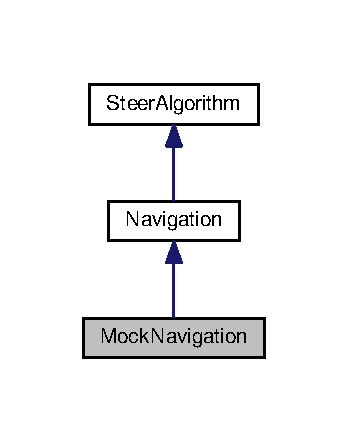
\includegraphics[width=167pt]{class_mock_navigation__inherit__graph}
\end{center}
\end{figure}


Collaboration diagram for Mock\+Navigation\+:
\nopagebreak
\begin{figure}[H]
\begin{center}
\leavevmode
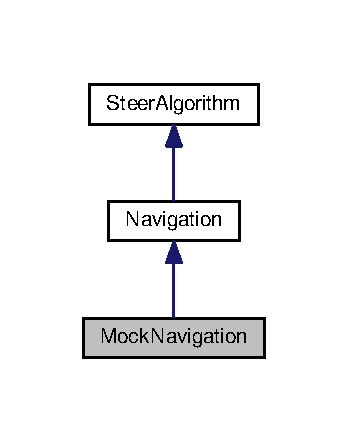
\includegraphics[width=167pt]{class_mock_navigation__coll__graph}
\end{center}
\end{figure}
\subsection*{Public Member Functions}
\begin{DoxyCompactItemize}
\item 
\hyperlink{class_mock_navigation_a54759f67f52b03841f44efe7926fff22}{Mock\+Navigation} ()\hypertarget{class_mock_navigation_a54759f67f52b03841f44efe7926fff22}{}\label{class_mock_navigation_a54759f67f52b03841f44efe7926fff22}

\begin{DoxyCompactList}\small\item\em Default constructor. \end{DoxyCompactList}\item 
\hyperlink{class_mock_navigation_acd53221a46f65f159ad53d22d3db1c51}{M\+O\+C\+K\+\_\+\+M\+E\+T\+H\+O\+D0} (\hyperlink{class_navigation_ab1469d74f4838a9d32a8647d22701f9f}{get\+Kp\+\_\+}, double())\hypertarget{class_mock_navigation_acd53221a46f65f159ad53d22d3db1c51}{}\label{class_mock_navigation_acd53221a46f65f159ad53d22d3db1c51}

\begin{DoxyCompactList}\small\item\em Mock get\+Kp\+\_\+. \end{DoxyCompactList}\item 
\hyperlink{class_mock_navigation_a5189068e3bbe0eeb377a119eaa8f0b62}{M\+O\+C\+K\+\_\+\+M\+E\+T\+H\+O\+D4} (\hyperlink{class_navigation_a0f83b511cec12a68f2c3466c40c5d3cb}{calculate}, double(double target\+Heading, double current\+Velocity, double set\+Point, int flag))\hypertarget{class_mock_navigation_a5189068e3bbe0eeb377a119eaa8f0b62}{}\label{class_mock_navigation_a5189068e3bbe0eeb377a119eaa8f0b62}

\begin{DoxyCompactList}\small\item\em Mock calculate method. \end{DoxyCompactList}\end{DoxyCompactItemize}
\subsection*{Additional Inherited Members}


\subsection{Detailed Description}
Mock \hyperlink{class_navigation}{Navigation} class. 

The documentation for this class was generated from the following file\+:\begin{DoxyCompactItemize}
\item 
/home/rajshinde/\+G\+M\+O\+C\+K/\+Robot\+\_\+\+Controller\+\_\+\+Module/include/\hyperlink{_mock_navigation_8hpp}{Mock\+Navigation.\+hpp}\end{DoxyCompactItemize}

\hypertarget{structgnuplotio_1_1_mode1_d}{}\section{gnuplotio\+:\+:Mode1D Struct Reference}
\label{structgnuplotio_1_1_mode1_d}\index{gnuplotio\+::\+Mode1D@{gnuplotio\+::\+Mode1D}}
\subsection*{Static Public Member Functions}
\begin{DoxyCompactItemize}
\item 
static std\+::string {\bfseries class\+\_\+name} ()\hypertarget{structgnuplotio_1_1_mode1_d_a508d170d84da4dfb7cd07eebad894b8f}{}\label{structgnuplotio_1_1_mode1_d_a508d170d84da4dfb7cd07eebad894b8f}

\end{DoxyCompactItemize}


The documentation for this struct was generated from the following file\+:\begin{DoxyCompactItemize}
\item 
/home/rajshinde/\+G\+M\+O\+C\+K/\+Robot\+\_\+\+Controller\+\_\+\+Module/include/gnuplot-\/iostream.\+h\end{DoxyCompactItemize}

\hypertarget{structgnuplotio_1_1_mode1_d_unwrap}{}\section{gnuplotio\+:\+:Mode1\+D\+Unwrap Struct Reference}
\label{structgnuplotio_1_1_mode1_d_unwrap}\index{gnuplotio\+::\+Mode1\+D\+Unwrap@{gnuplotio\+::\+Mode1\+D\+Unwrap}}
\subsection*{Static Public Member Functions}
\begin{DoxyCompactItemize}
\item 
static std\+::string {\bfseries class\+\_\+name} ()\hypertarget{structgnuplotio_1_1_mode1_d_unwrap_a2350096ad4d8b668f6df56c32cab69b6}{}\label{structgnuplotio_1_1_mode1_d_unwrap_a2350096ad4d8b668f6df56c32cab69b6}

\end{DoxyCompactItemize}


The documentation for this struct was generated from the following file\+:\begin{DoxyCompactItemize}
\item 
/home/rajshinde/\+G\+M\+O\+C\+K/\+Robot\+\_\+\+Controller\+\_\+\+Module/include/gnuplot-\/iostream.\+h\end{DoxyCompactItemize}

\hypertarget{structgnuplotio_1_1_mode2_d}{}\section{gnuplotio\+:\+:Mode2D Struct Reference}
\label{structgnuplotio_1_1_mode2_d}\index{gnuplotio\+::\+Mode2D@{gnuplotio\+::\+Mode2D}}
\subsection*{Static Public Member Functions}
\begin{DoxyCompactItemize}
\item 
static std\+::string {\bfseries class\+\_\+name} ()\hypertarget{structgnuplotio_1_1_mode2_d_aaf35c9cd117de8bc5dbc2d5ec1224232}{}\label{structgnuplotio_1_1_mode2_d_aaf35c9cd117de8bc5dbc2d5ec1224232}

\end{DoxyCompactItemize}


The documentation for this struct was generated from the following file\+:\begin{DoxyCompactItemize}
\item 
/home/rajshinde/\+G\+M\+O\+C\+K/\+Robot\+\_\+\+Controller\+\_\+\+Module/include/gnuplot-\/iostream.\+h\end{DoxyCompactItemize}

\hypertarget{structgnuplotio_1_1_mode2_d_unwrap}{}\section{gnuplotio\+:\+:Mode2\+D\+Unwrap Struct Reference}
\label{structgnuplotio_1_1_mode2_d_unwrap}\index{gnuplotio\+::\+Mode2\+D\+Unwrap@{gnuplotio\+::\+Mode2\+D\+Unwrap}}
\subsection*{Static Public Member Functions}
\begin{DoxyCompactItemize}
\item 
static std\+::string {\bfseries class\+\_\+name} ()\hypertarget{structgnuplotio_1_1_mode2_d_unwrap_ab2f533c9ceb52cfecaa161c64316deb9}{}\label{structgnuplotio_1_1_mode2_d_unwrap_ab2f533c9ceb52cfecaa161c64316deb9}

\end{DoxyCompactItemize}


The documentation for this struct was generated from the following file\+:\begin{DoxyCompactItemize}
\item 
/home/rajshinde/\+G\+M\+O\+C\+K/\+Robot\+\_\+\+Controller\+\_\+\+Module/include/gnuplot-\/iostream.\+h\end{DoxyCompactItemize}

\hypertarget{structgnuplotio_1_1_mode_auto}{}\section{gnuplotio\+:\+:Mode\+Auto Struct Reference}
\label{structgnuplotio_1_1_mode_auto}\index{gnuplotio\+::\+Mode\+Auto@{gnuplotio\+::\+Mode\+Auto}}
\subsection*{Static Public Member Functions}
\begin{DoxyCompactItemize}
\item 
static std\+::string {\bfseries class\+\_\+name} ()\hypertarget{structgnuplotio_1_1_mode_auto_ac73f89a782ac32dd8bc7b8f7a7581523}{}\label{structgnuplotio_1_1_mode_auto_ac73f89a782ac32dd8bc7b8f7a7581523}

\end{DoxyCompactItemize}


The documentation for this struct was generated from the following file\+:\begin{DoxyCompactItemize}
\item 
/home/rajshinde/\+G\+M\+O\+C\+K/\+Robot\+\_\+\+Controller\+\_\+\+Module/include/gnuplot-\/iostream.\+h\end{DoxyCompactItemize}

\hypertarget{structgnuplotio_1_1_mode_auto_decoder}{}\section{gnuplotio\+:\+:Mode\+Auto\+Decoder$<$ T, Enable $>$ Struct Template Reference}
\label{structgnuplotio_1_1_mode_auto_decoder}\index{gnuplotio\+::\+Mode\+Auto\+Decoder$<$ T, Enable $>$@{gnuplotio\+::\+Mode\+Auto\+Decoder$<$ T, Enable $>$}}


The documentation for this struct was generated from the following file\+:\begin{DoxyCompactItemize}
\item 
/home/rajshinde/\+G\+M\+O\+C\+K/\+Robot\+\_\+\+Controller\+\_\+\+Module/include/gnuplot-\/iostream.\+h\end{DoxyCompactItemize}

\hypertarget{structgnuplotio_1_1_mode_binary}{}\section{gnuplotio\+:\+:Mode\+Binary Struct Reference}
\label{structgnuplotio_1_1_mode_binary}\index{gnuplotio\+::\+Mode\+Binary@{gnuplotio\+::\+Mode\+Binary}}
\subsection*{Static Public Attributes}
\begin{DoxyCompactItemize}
\item 
static const bool {\bfseries is\+\_\+text} = 0\hypertarget{structgnuplotio_1_1_mode_binary_ac89064b5df24f7ef4d765fdfde4fd1b6}{}\label{structgnuplotio_1_1_mode_binary_ac89064b5df24f7ef4d765fdfde4fd1b6}

\item 
static const bool {\bfseries is\+\_\+binfmt} = 0\hypertarget{structgnuplotio_1_1_mode_binary_aee724034dc3372b8e12b1187507bf136}{}\label{structgnuplotio_1_1_mode_binary_aee724034dc3372b8e12b1187507bf136}

\item 
static const bool {\bfseries is\+\_\+size} = 0\hypertarget{structgnuplotio_1_1_mode_binary_a6eae25ea662362bbb88bc987d6025290}{}\label{structgnuplotio_1_1_mode_binary_a6eae25ea662362bbb88bc987d6025290}

\end{DoxyCompactItemize}


The documentation for this struct was generated from the following file\+:\begin{DoxyCompactItemize}
\item 
/home/rajshinde/\+G\+M\+O\+C\+K/\+Robot\+\_\+\+Controller\+\_\+\+Module/include/gnuplot-\/iostream.\+h\end{DoxyCompactItemize}

\hypertarget{structgnuplotio_1_1_mode_binfmt}{}\section{gnuplotio\+:\+:Mode\+Binfmt Struct Reference}
\label{structgnuplotio_1_1_mode_binfmt}\index{gnuplotio\+::\+Mode\+Binfmt@{gnuplotio\+::\+Mode\+Binfmt}}
\subsection*{Static Public Attributes}
\begin{DoxyCompactItemize}
\item 
static const bool {\bfseries is\+\_\+text} = 0\hypertarget{structgnuplotio_1_1_mode_binfmt_a7ab187fe922cac23b0d39ade81e5eb56}{}\label{structgnuplotio_1_1_mode_binfmt_a7ab187fe922cac23b0d39ade81e5eb56}

\item 
static const bool {\bfseries is\+\_\+binfmt} = 1\hypertarget{structgnuplotio_1_1_mode_binfmt_ab0d5d3718364cdea0347f93ec121d841}{}\label{structgnuplotio_1_1_mode_binfmt_ab0d5d3718364cdea0347f93ec121d841}

\item 
static const bool {\bfseries is\+\_\+size} = 0\hypertarget{structgnuplotio_1_1_mode_binfmt_a40a5a8ee815d6a5e9a3c30c8290a6967}{}\label{structgnuplotio_1_1_mode_binfmt_a40a5a8ee815d6a5e9a3c30c8290a6967}

\end{DoxyCompactItemize}


The documentation for this struct was generated from the following file\+:\begin{DoxyCompactItemize}
\item 
/home/rajshinde/\+G\+M\+O\+C\+K/\+Robot\+\_\+\+Controller\+\_\+\+Module/include/gnuplot-\/iostream.\+h\end{DoxyCompactItemize}

\hypertarget{structgnuplotio_1_1_mode_size}{}\section{gnuplotio\+:\+:Mode\+Size Struct Reference}
\label{structgnuplotio_1_1_mode_size}\index{gnuplotio\+::\+Mode\+Size@{gnuplotio\+::\+Mode\+Size}}
\subsection*{Static Public Attributes}
\begin{DoxyCompactItemize}
\item 
static const bool {\bfseries is\+\_\+text} = 0\hypertarget{structgnuplotio_1_1_mode_size_aa01840f76877ae7c8bad254dae28e32c}{}\label{structgnuplotio_1_1_mode_size_aa01840f76877ae7c8bad254dae28e32c}

\item 
static const bool {\bfseries is\+\_\+binfmt} = 0\hypertarget{structgnuplotio_1_1_mode_size_ac5243e8e4910f2f6a2724b9fc0de4ff9}{}\label{structgnuplotio_1_1_mode_size_ac5243e8e4910f2f6a2724b9fc0de4ff9}

\item 
static const bool {\bfseries is\+\_\+size} = 1\hypertarget{structgnuplotio_1_1_mode_size_aa20ae9f1ce222504489db33d13eb46c0}{}\label{structgnuplotio_1_1_mode_size_aa20ae9f1ce222504489db33d13eb46c0}

\end{DoxyCompactItemize}


The documentation for this struct was generated from the following file\+:\begin{DoxyCompactItemize}
\item 
/home/rajshinde/\+G\+M\+O\+C\+K/\+Robot\+\_\+\+Controller\+\_\+\+Module/include/gnuplot-\/iostream.\+h\end{DoxyCompactItemize}

\hypertarget{structgnuplotio_1_1_mode_text}{}\section{gnuplotio\+:\+:Mode\+Text Struct Reference}
\label{structgnuplotio_1_1_mode_text}\index{gnuplotio\+::\+Mode\+Text@{gnuplotio\+::\+Mode\+Text}}
\subsection*{Static Public Attributes}
\begin{DoxyCompactItemize}
\item 
static const bool {\bfseries is\+\_\+text} = 1\hypertarget{structgnuplotio_1_1_mode_text_a7083d8977c354a036a7c542bf99d3d52}{}\label{structgnuplotio_1_1_mode_text_a7083d8977c354a036a7c542bf99d3d52}

\item 
static const bool {\bfseries is\+\_\+binfmt} = 0\hypertarget{structgnuplotio_1_1_mode_text_a4c771363d894ae64d6af961ffde35126}{}\label{structgnuplotio_1_1_mode_text_a4c771363d894ae64d6af961ffde35126}

\item 
static const bool {\bfseries is\+\_\+size} = 0\hypertarget{structgnuplotio_1_1_mode_text_aaffc1e7bb26c6d1404cb5a3f03f13be9}{}\label{structgnuplotio_1_1_mode_text_aaffc1e7bb26c6d1404cb5a3f03f13be9}

\end{DoxyCompactItemize}


The documentation for this struct was generated from the following file\+:\begin{DoxyCompactItemize}
\item 
/home/rajshinde/\+G\+M\+O\+C\+K/\+Robot\+\_\+\+Controller\+\_\+\+Module/include/gnuplot-\/iostream.\+h\end{DoxyCompactItemize}

\hypertarget{class_navigation}{}\section{Navigation Class Reference}
\label{class_navigation}\index{Navigation@{Navigation}}


Class \hyperlink{class_navigation}{Navigation} Contains the methods of steer Algorithm.  




{\ttfamily \#include $<$Navigation.\+hpp$>$}



Inheritance diagram for Navigation\+:
\nopagebreak
\begin{figure}[H]
\begin{center}
\leavevmode
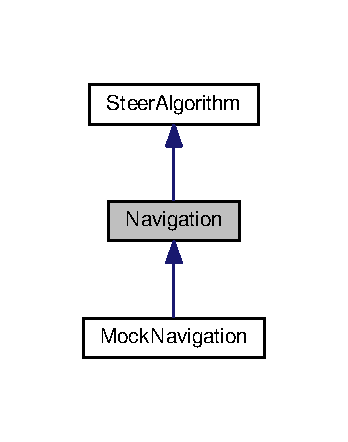
\includegraphics[width=167pt]{class_navigation__inherit__graph}
\end{center}
\end{figure}


Collaboration diagram for Navigation\+:
\nopagebreak
\begin{figure}[H]
\begin{center}
\leavevmode
\includegraphics[width=161pt]{class_navigation__coll__graph}
\end{center}
\end{figure}
\subsection*{Public Member Functions}
\begin{DoxyCompactItemize}
\item 
\hyperlink{class_navigation_a81fdffdefe46340da5fa6c570066b42b}{Navigation} ()\hypertarget{class_navigation_a81fdffdefe46340da5fa6c570066b42b}{}\label{class_navigation_a81fdffdefe46340da5fa6c570066b42b}

\begin{DoxyCompactList}\small\item\em Constructor of class \hyperlink{class_navigation}{Navigation}. \end{DoxyCompactList}\item 
\hyperlink{class_navigation_addd4022d716df48f4e55a1db69361ba7}{$\sim$\+Navigation} ()\hypertarget{class_navigation_addd4022d716df48f4e55a1db69361ba7}{}\label{class_navigation_addd4022d716df48f4e55a1db69361ba7}

\begin{DoxyCompactList}\small\item\em Destructor of class \hyperlink{class_navigation}{Navigation}. \end{DoxyCompactList}\item 
double \hyperlink{class_navigation_a0f83b511cec12a68f2c3466c40c5d3cb}{calculate} (double target\+Heading, double current\+Velocity, double set\+Point, int flag)
\begin{DoxyCompactList}\small\item\em Function to calculate new velocity in m/s with a P\+ID Algorithm using kp, ki \& kd. \end{DoxyCompactList}\item 
bool \hyperlink{class_navigation_af6a893750980a747eccf700e22d2cbae}{setup\+Graph} ()
\begin{DoxyCompactList}\small\item\em Function to set graph parameters. \end{DoxyCompactList}\item 
bool \hyperlink{class_navigation_a8a2193deb9aff2804453b8cf585691c0}{display} (int loc, double current\+Velocity, double new\+Velocity, double heading, double target\+Heading)
\begin{DoxyCompactList}\small\item\em Function to display on Terminal. \end{DoxyCompactList}\item 
bool \hyperlink{class_navigation_a95c972751207516ff0d85af6d42e75f7}{draw\+Graph} (std\+::vector$<$ std\+::pair$<$ double, double $>$$>$ points, std\+::vector$<$ std\+::pair$<$ double, double $>$$>$ points\+Velocity, double new\+Velocity, double temp\+Heading)
\begin{DoxyCompactList}\small\item\em Function to draw graphs in gnuplot. \end{DoxyCompactList}\item 
double \hyperlink{class_navigation_ab1469d74f4838a9d32a8647d22701f9f}{get\+Kp\+\_\+} ()
\begin{DoxyCompactList}\small\item\em Function to get kp\+\_\+. \end{DoxyCompactList}\item 
double \hyperlink{class_navigation_a1a84392d6cce3f60df452ab482b5647c}{get\+Ki\+\_\+} ()
\begin{DoxyCompactList}\small\item\em Function to get ki\+\_\+. \end{DoxyCompactList}\item 
double \hyperlink{class_navigation_ac6441bb601483166ef7a8081b76f634d}{get\+Kd\+\_\+} ()
\begin{DoxyCompactList}\small\item\em Function to get kd\+\_\+. \end{DoxyCompactList}\item 
bool \hyperlink{class_navigation_a6dd95f46ff4ecc69895452a1879c30af}{set\+Kp\+\_\+} (double kp)
\begin{DoxyCompactList}\small\item\em Function to set kp\+\_\+. \end{DoxyCompactList}\item 
bool \hyperlink{class_navigation_a539d10206ceb162171e39c36e8aa8f0f}{set\+Ki\+\_\+} (double ki)
\begin{DoxyCompactList}\small\item\em Function to set ki\+\_\+. \end{DoxyCompactList}\item 
bool \hyperlink{class_navigation_a4986e4357d9707ddf92cf8f559ef3dce}{set\+Kd\+\_\+} (double kd)
\begin{DoxyCompactList}\small\item\em Function to set kd\+\_\+. \end{DoxyCompactList}\end{DoxyCompactItemize}
\subsection*{Public Attributes}
\begin{DoxyCompactItemize}
\item 
bool {\bfseries motor\+Direction} = true\hypertarget{class_navigation_ad7d7a5d5d1abe99e6b0f31ddb4794252}{}\label{class_navigation_ad7d7a5d5d1abe99e6b0f31ddb4794252}

\end{DoxyCompactItemize}


\subsection{Detailed Description}
Class \hyperlink{class_navigation}{Navigation} Contains the methods of steer Algorithm. 

\subsection{Member Function Documentation}
\index{Navigation@{Navigation}!calculate@{calculate}}
\index{calculate@{calculate}!Navigation@{Navigation}}
\subsubsection[{\texorpdfstring{calculate(double target\+Heading, double current\+Velocity, double set\+Point, int flag)}{calculate(double targetHeading, double currentVelocity, double setPoint, int flag)}}]{\setlength{\rightskip}{0pt plus 5cm}double Navigation\+::calculate (
\begin{DoxyParamCaption}
\item[{double}]{target\+Heading, }
\item[{double}]{current\+Velocity, }
\item[{double}]{set\+Point, }
\item[{int}]{flag}
\end{DoxyParamCaption}
)}\hypertarget{class_navigation_a0f83b511cec12a68f2c3466c40c5d3cb}{}\label{class_navigation_a0f83b511cec12a68f2c3466c40c5d3cb}


Function to calculate new velocity in m/s with a P\+ID Algorithm using kp, ki \& kd. 


\begin{DoxyParams}{Parameters}
{\em double} & target\+Heading, Target heading of the robot \\
\hline
{\em double} & current\+Velocity, current velocity of robot \\
\hline
{\em double} & set\+Point, Target Velocity \\
\hline
{\em int} & flag, to enable while \\
\hline
\end{DoxyParams}
\begin{DoxyReturn}{Returns}
double new\+Velocity 
\end{DoxyReturn}
\index{Navigation@{Navigation}!display@{display}}
\index{display@{display}!Navigation@{Navigation}}
\subsubsection[{\texorpdfstring{display(int loc, double current\+Velocity, double new\+Velocity, double heading, double target\+Heading)}{display(int loc, double currentVelocity, double newVelocity, double heading, double targetHeading)}}]{\setlength{\rightskip}{0pt plus 5cm}bool Navigation\+::display (
\begin{DoxyParamCaption}
\item[{int}]{loc, }
\item[{double}]{current\+Velocity, }
\item[{double}]{new\+Velocity, }
\item[{double}]{heading, }
\item[{double}]{target\+Heading}
\end{DoxyParamCaption}
)}\hypertarget{class_navigation_a8a2193deb9aff2804453b8cf585691c0}{}\label{class_navigation_a8a2193deb9aff2804453b8cf585691c0}


Function to display on Terminal. 


\begin{DoxyParams}{Parameters}
{\em int} & loc \\
\hline
{\em double} & current\+Velocity \\
\hline
{\em double} & new\+Velocity \\
\hline
{\em double} & heading \\
\hline
{\em double} & target\+Heading \\
\hline
\end{DoxyParams}
\begin{DoxyReturn}{Returns}
none 
\end{DoxyReturn}
\index{Navigation@{Navigation}!draw\+Graph@{draw\+Graph}}
\index{draw\+Graph@{draw\+Graph}!Navigation@{Navigation}}
\subsubsection[{\texorpdfstring{draw\+Graph(std\+::vector$<$ std\+::pair$<$ double, double $>$$>$ points, std\+::vector$<$ std\+::pair$<$ double, double $>$$>$ points\+Velocity, double new\+Velocity, double temp\+Heading)}{drawGraph(std::vector< std::pair< double, double >> points, std::vector< std::pair< double, double >> pointsVelocity, double newVelocity, double tempHeading)}}]{\setlength{\rightskip}{0pt plus 5cm}bool Navigation\+::draw\+Graph (
\begin{DoxyParamCaption}
\item[{std\+::vector$<$ std\+::pair$<$ double, double $>$$>$}]{points, }
\item[{std\+::vector$<$ std\+::pair$<$ double, double $>$$>$}]{points\+Velocity, }
\item[{double}]{new\+Velocity, }
\item[{double}]{temp\+Heading}
\end{DoxyParamCaption}
)}\hypertarget{class_navigation_a95c972751207516ff0d85af6d42e75f7}{}\label{class_navigation_a95c972751207516ff0d85af6d42e75f7}


Function to draw graphs in gnuplot. 


\begin{DoxyParams}{Parameters}
{\em vector$<$pair$<$double,double$>$$>$} & points \\
\hline
{\em vector$<$pair$<$double,double$>$$>$} & points\+Velocity \\
\hline
{\em double} & new\+Velocity \\
\hline
{\em double} & temp\+Heading \\
\hline
\end{DoxyParams}
\begin{DoxyReturn}{Returns}
none 
\end{DoxyReturn}
\index{Navigation@{Navigation}!get\+Kd\+\_\+@{get\+Kd\+\_\+}}
\index{get\+Kd\+\_\+@{get\+Kd\+\_\+}!Navigation@{Navigation}}
\subsubsection[{\texorpdfstring{get\+Kd\+\_\+()}{getKd_()}}]{\setlength{\rightskip}{0pt plus 5cm}double Navigation\+::get\+Kd\+\_\+ (
\begin{DoxyParamCaption}
{}
\end{DoxyParamCaption}
)}\hypertarget{class_navigation_ac6441bb601483166ef7a8081b76f634d}{}\label{class_navigation_ac6441bb601483166ef7a8081b76f634d}


Function to get kd\+\_\+. 


\begin{DoxyParams}{Parameters}
{\em none} & \\
\hline
\end{DoxyParams}
\begin{DoxyReturn}{Returns}
double 
\end{DoxyReturn}
\index{Navigation@{Navigation}!get\+Ki\+\_\+@{get\+Ki\+\_\+}}
\index{get\+Ki\+\_\+@{get\+Ki\+\_\+}!Navigation@{Navigation}}
\subsubsection[{\texorpdfstring{get\+Ki\+\_\+()}{getKi_()}}]{\setlength{\rightskip}{0pt plus 5cm}double Navigation\+::get\+Ki\+\_\+ (
\begin{DoxyParamCaption}
{}
\end{DoxyParamCaption}
)}\hypertarget{class_navigation_a1a84392d6cce3f60df452ab482b5647c}{}\label{class_navigation_a1a84392d6cce3f60df452ab482b5647c}


Function to get ki\+\_\+. 


\begin{DoxyParams}{Parameters}
{\em none} & \\
\hline
\end{DoxyParams}
\begin{DoxyReturn}{Returns}
double 
\end{DoxyReturn}
\index{Navigation@{Navigation}!get\+Kp\+\_\+@{get\+Kp\+\_\+}}
\index{get\+Kp\+\_\+@{get\+Kp\+\_\+}!Navigation@{Navigation}}
\subsubsection[{\texorpdfstring{get\+Kp\+\_\+()}{getKp_()}}]{\setlength{\rightskip}{0pt plus 5cm}double Navigation\+::get\+Kp\+\_\+ (
\begin{DoxyParamCaption}
{}
\end{DoxyParamCaption}
)}\hypertarget{class_navigation_ab1469d74f4838a9d32a8647d22701f9f}{}\label{class_navigation_ab1469d74f4838a9d32a8647d22701f9f}


Function to get kp\+\_\+. 


\begin{DoxyParams}{Parameters}
{\em none} & \\
\hline
\end{DoxyParams}
\begin{DoxyReturn}{Returns}
double 
\end{DoxyReturn}
\index{Navigation@{Navigation}!set\+Kd\+\_\+@{set\+Kd\+\_\+}}
\index{set\+Kd\+\_\+@{set\+Kd\+\_\+}!Navigation@{Navigation}}
\subsubsection[{\texorpdfstring{set\+Kd\+\_\+(double kd)}{setKd_(double kd)}}]{\setlength{\rightskip}{0pt plus 5cm}bool Navigation\+::set\+Kd\+\_\+ (
\begin{DoxyParamCaption}
\item[{double}]{kd}
\end{DoxyParamCaption}
)}\hypertarget{class_navigation_a4986e4357d9707ddf92cf8f559ef3dce}{}\label{class_navigation_a4986e4357d9707ddf92cf8f559ef3dce}


Function to set kd\+\_\+. 


\begin{DoxyParams}{Parameters}
{\em double} & kd \\
\hline
\end{DoxyParams}
\begin{DoxyReturn}{Returns}
boolean true 
\end{DoxyReturn}
\index{Navigation@{Navigation}!set\+Ki\+\_\+@{set\+Ki\+\_\+}}
\index{set\+Ki\+\_\+@{set\+Ki\+\_\+}!Navigation@{Navigation}}
\subsubsection[{\texorpdfstring{set\+Ki\+\_\+(double ki)}{setKi_(double ki)}}]{\setlength{\rightskip}{0pt plus 5cm}bool Navigation\+::set\+Ki\+\_\+ (
\begin{DoxyParamCaption}
\item[{double}]{ki}
\end{DoxyParamCaption}
)}\hypertarget{class_navigation_a539d10206ceb162171e39c36e8aa8f0f}{}\label{class_navigation_a539d10206ceb162171e39c36e8aa8f0f}


Function to set ki\+\_\+. 


\begin{DoxyParams}{Parameters}
{\em double} & ki \\
\hline
\end{DoxyParams}
\begin{DoxyReturn}{Returns}
boolean true 
\end{DoxyReturn}
\index{Navigation@{Navigation}!set\+Kp\+\_\+@{set\+Kp\+\_\+}}
\index{set\+Kp\+\_\+@{set\+Kp\+\_\+}!Navigation@{Navigation}}
\subsubsection[{\texorpdfstring{set\+Kp\+\_\+(double kp)}{setKp_(double kp)}}]{\setlength{\rightskip}{0pt plus 5cm}bool Navigation\+::set\+Kp\+\_\+ (
\begin{DoxyParamCaption}
\item[{double}]{kp}
\end{DoxyParamCaption}
)}\hypertarget{class_navigation_a6dd95f46ff4ecc69895452a1879c30af}{}\label{class_navigation_a6dd95f46ff4ecc69895452a1879c30af}


Function to set kp\+\_\+. 


\begin{DoxyParams}{Parameters}
{\em double} & kp \\
\hline
\end{DoxyParams}
\begin{DoxyReturn}{Returns}
boolean true 
\end{DoxyReturn}
\index{Navigation@{Navigation}!setup\+Graph@{setup\+Graph}}
\index{setup\+Graph@{setup\+Graph}!Navigation@{Navigation}}
\subsubsection[{\texorpdfstring{setup\+Graph()}{setupGraph()}}]{\setlength{\rightskip}{0pt plus 5cm}bool Navigation\+::setup\+Graph (
\begin{DoxyParamCaption}
{}
\end{DoxyParamCaption}
)}\hypertarget{class_navigation_af6a893750980a747eccf700e22d2cbae}{}\label{class_navigation_af6a893750980a747eccf700e22d2cbae}


Function to set graph parameters. 


\begin{DoxyParams}{Parameters}
{\em none} & \\
\hline
\end{DoxyParams}
\begin{DoxyReturn}{Returns}
none 
\end{DoxyReturn}


The documentation for this class was generated from the following files\+:\begin{DoxyCompactItemize}
\item 
/home/rajshinde/\+G\+M\+O\+C\+K/\+Robot\+\_\+\+Controller\+\_\+\+Module/include/\hyperlink{_navigation_8hpp}{Navigation.\+hpp}\item 
/home/rajshinde/\+G\+M\+O\+C\+K/\+Robot\+\_\+\+Controller\+\_\+\+Module/app/\hyperlink{_navigation_8cpp}{Navigation.\+cpp}\end{DoxyCompactItemize}

\hypertarget{classgnuplotio_1_1_pair_of_range}{}\section{gnuplotio\+:\+:Pair\+Of\+Range$<$ RT, RU $>$ Class Template Reference}
\label{classgnuplotio_1_1_pair_of_range}\index{gnuplotio\+::\+Pair\+Of\+Range$<$ R\+T, R\+U $>$@{gnuplotio\+::\+Pair\+Of\+Range$<$ R\+T, R\+U $>$}}
\subsection*{Public Types}
\begin{DoxyCompactItemize}
\item 
typedef std\+::pair$<$ typename R\+T\+::value\+\_\+type, typename R\+U\+::value\+\_\+type $>$ {\bfseries value\+\_\+type}\hypertarget{classgnuplotio_1_1_pair_of_range_a0cc8b0cc4d9c3377c43843ed9a658eeb}{}\label{classgnuplotio_1_1_pair_of_range_a0cc8b0cc4d9c3377c43843ed9a658eeb}

\item 
typedef \hyperlink{classgnuplotio_1_1_pair_of_range}{Pair\+Of\+Range}$<$ typename R\+T\+::subiter\+\_\+type, typename R\+U\+::subiter\+\_\+type $>$ {\bfseries subiter\+\_\+type}\hypertarget{classgnuplotio_1_1_pair_of_range_a6a7bf8a5dd4ca0563eb71b1156d6cd9f}{}\label{classgnuplotio_1_1_pair_of_range_a6a7bf8a5dd4ca0563eb71b1156d6cd9f}

\end{DoxyCompactItemize}
\subsection*{Public Member Functions}
\begin{DoxyCompactItemize}
\item 
{\bfseries Pair\+Of\+Range} (const RT \&\+\_\+l, const RU \&\+\_\+r)\hypertarget{classgnuplotio_1_1_pair_of_range_a15055ed8b1c0af8febf20f5a24d7dc05}{}\label{classgnuplotio_1_1_pair_of_range_a15055ed8b1c0af8febf20f5a24d7dc05}

\item 
bool {\bfseries is\+\_\+end} () const \hypertarget{classgnuplotio_1_1_pair_of_range_a1995b2f3b4c00fa9d0b4705aac4cb3ac}{}\label{classgnuplotio_1_1_pair_of_range_a1995b2f3b4c00fa9d0b4705aac4cb3ac}

\item 
void {\bfseries inc} ()\hypertarget{classgnuplotio_1_1_pair_of_range_adbb8ab0fb9f7245262041dd20444b96a}{}\label{classgnuplotio_1_1_pair_of_range_adbb8ab0fb9f7245262041dd20444b96a}

\item 
value\+\_\+type {\bfseries deref} () const \hypertarget{classgnuplotio_1_1_pair_of_range_ab4cde941279940d87a4182706ed5d88d}{}\label{classgnuplotio_1_1_pair_of_range_ab4cde941279940d87a4182706ed5d88d}

\item 
\hyperlink{classgnuplotio_1_1_pair_of_range}{subiter\+\_\+type} {\bfseries deref\+\_\+subiter} () const \hypertarget{classgnuplotio_1_1_pair_of_range_abba540b498666a006f1e31cf0cbf24c5}{}\label{classgnuplotio_1_1_pair_of_range_abba540b498666a006f1e31cf0cbf24c5}

\end{DoxyCompactItemize}
\subsection*{Static Public Attributes}
\begin{DoxyCompactItemize}
\item 
static const bool {\bfseries is\+\_\+container} = R\+T\+::is\+\_\+container \&\& R\+U\+::is\+\_\+container\hypertarget{classgnuplotio_1_1_pair_of_range_ab49c6567f0fa6a82fa2a6245fd964659}{}\label{classgnuplotio_1_1_pair_of_range_ab49c6567f0fa6a82fa2a6245fd964659}

\end{DoxyCompactItemize}
\subsection*{Friends}
\begin{DoxyCompactItemize}
\item 
{\footnotesize template$<$typename T , typename U , typename Print\+Mode $>$ }\\void {\bfseries deref\+\_\+and\+\_\+print} (std\+::ostream \&, const \hyperlink{classgnuplotio_1_1_pair_of_range}{Pair\+Of\+Range}$<$ T, U $>$ \&, Print\+Mode)\hypertarget{classgnuplotio_1_1_pair_of_range_aada62f803432f04aff66f3c609329520}{}\label{classgnuplotio_1_1_pair_of_range_aada62f803432f04aff66f3c609329520}

\end{DoxyCompactItemize}


The documentation for this class was generated from the following file\+:\begin{DoxyCompactItemize}
\item 
/home/rajshinde/\+G\+M\+O\+C\+K/\+Robot\+\_\+\+Controller\+\_\+\+Module/include/gnuplot-\/iostream.\+h\end{DoxyCompactItemize}

\hypertarget{classgnuplotio_1_1plotting__empty__container}{}\section{gnuplotio\+:\+:plotting\+\_\+empty\+\_\+container Class Reference}
\label{classgnuplotio_1_1plotting__empty__container}\index{gnuplotio\+::plotting\+\_\+empty\+\_\+container@{gnuplotio\+::plotting\+\_\+empty\+\_\+container}}


Inheritance diagram for gnuplotio\+:\+:plotting\+\_\+empty\+\_\+container\+:
\nopagebreak
\begin{figure}[H]
\begin{center}
\leavevmode
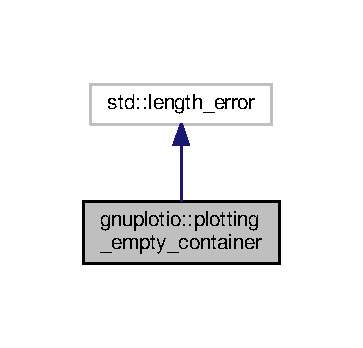
\includegraphics[width=174pt]{classgnuplotio_1_1plotting__empty__container__inherit__graph}
\end{center}
\end{figure}


Collaboration diagram for gnuplotio\+:\+:plotting\+\_\+empty\+\_\+container\+:
\nopagebreak
\begin{figure}[H]
\begin{center}
\leavevmode
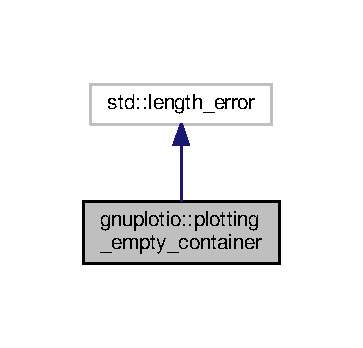
\includegraphics[width=174pt]{classgnuplotio_1_1plotting__empty__container__coll__graph}
\end{center}
\end{figure}


The documentation for this class was generated from the following file\+:\begin{DoxyCompactItemize}
\item 
/home/rajshinde/\+G\+M\+O\+C\+K/\+Robot\+\_\+\+Controller\+\_\+\+Module/include/gnuplot-\/iostream.\+h\end{DoxyCompactItemize}

\hypertarget{class_steer_algorithm}{}\section{Steer\+Algorithm Class Reference}
\label{class_steer_algorithm}\index{Steer\+Algorithm@{Steer\+Algorithm}}


Class \hyperlink{class_steer_algorithm}{Steer\+Algorithm} contains the methods of the Steering Algorithm.  




{\ttfamily \#include $<$Steer\+Algorithm.\+hpp$>$}



Inheritance diagram for Steer\+Algorithm\+:
\nopagebreak
\begin{figure}[H]
\begin{center}
\leavevmode
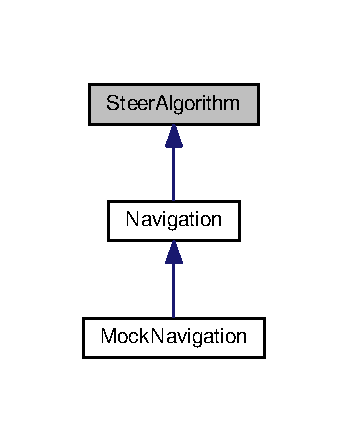
\includegraphics[width=167pt]{class_steer_algorithm__inherit__graph}
\end{center}
\end{figure}
\subsection*{Public Member Functions}
\begin{DoxyCompactItemize}
\item 
\hyperlink{class_steer_algorithm_af64dd94816ab9d00d85227a42b26a3e8}{Steer\+Algorithm} ()\hypertarget{class_steer_algorithm_af64dd94816ab9d00d85227a42b26a3e8}{}\label{class_steer_algorithm_af64dd94816ab9d00d85227a42b26a3e8}

\begin{DoxyCompactList}\small\item\em Constructor of class \hyperlink{class_steer_algorithm}{Steer\+Algorithm}. \end{DoxyCompactList}\item 
\hyperlink{class_steer_algorithm_a37dd2ef0ed856582aaacc103a6cd6700}{$\sim$\+Steer\+Algorithm} ()\hypertarget{class_steer_algorithm_a37dd2ef0ed856582aaacc103a6cd6700}{}\label{class_steer_algorithm_a37dd2ef0ed856582aaacc103a6cd6700}

\begin{DoxyCompactList}\small\item\em Destructor of class \hyperlink{class_steer_algorithm}{Steer\+Algorithm}. \end{DoxyCompactList}\item 
double \hyperlink{class_steer_algorithm_a3ab412260c2457994f1180623862584b}{get\+Corr\+Radius} ()
\begin{DoxyCompactList}\small\item\em Function to get corresponding radius in meters. \end{DoxyCompactList}\item 
bool \hyperlink{class_steer_algorithm_a2314874a6f7252823e994e0e8b0a6b38}{set\+Corr\+Radius} (double r)
\begin{DoxyCompactList}\small\item\em Function to set corresponding radius in meters. \end{DoxyCompactList}\item 
double \hyperlink{class_steer_algorithm_a17ff78af17e900f752237d274bcf751d}{arc\+Length} (double diff\+Angle, double corr\+Radius)
\begin{DoxyCompactList}\small\item\em Function to calculate the length of arc in meters to be traced in order to head in target direction. \end{DoxyCompactList}\item 
double \hyperlink{class_steer_algorithm_a6067af69593713f561890ae8ad23f5ff}{change\+Wheel\+Angles} (double corr\+Radius, double shaft\+Length, double shaft\+Distance)
\begin{DoxyCompactList}\small\item\em Function to calculate the angles in degrees for left and right wheels as per ackermann model, and then feed them to corresponding servo. \end{DoxyCompactList}\item 
bool \hyperlink{class_steer_algorithm_ab251b6fd1f88fb7a526b0d55cd12625b}{reset\+Wheel} ()
\begin{DoxyCompactList}\small\item\em Function to set wheel angles to 0. \end{DoxyCompactList}\item 
double \hyperlink{class_steer_algorithm_aefdb433f65c47bf6e0d6af5de98c8f5a}{turn\+Time} (double arclength, double new\+Velocity)
\begin{DoxyCompactList}\small\item\em Function to calculate time in seconds required to turn or keep wheels at the an angle. \end{DoxyCompactList}\end{DoxyCompactItemize}
\subsection*{Public Attributes}
\begin{DoxyCompactItemize}
\item 
const double {\bfseries shaft\+Length} = 4\hypertarget{class_steer_algorithm_a9d5bc20acba39f0e53c3d0f6fc280433}{}\label{class_steer_algorithm_a9d5bc20acba39f0e53c3d0f6fc280433}

\item 
const double {\bfseries shaft\+Distance} = 8\hypertarget{class_steer_algorithm_a38bc87552a30e8eda8f647cf341c9657}{}\label{class_steer_algorithm_a38bc87552a30e8eda8f647cf341c9657}

\item 
const double {\bfseries max\+Turn\+Velocity} = 20\hypertarget{class_steer_algorithm_acfce52839329f0ebb316f633494466e1}{}\label{class_steer_algorithm_acfce52839329f0ebb316f633494466e1}

\item 
double {\bfseries heading}\hypertarget{class_steer_algorithm_ada73b1f087245af5cda5d1d6b9be7d31}{}\label{class_steer_algorithm_ada73b1f087245af5cda5d1d6b9be7d31}

\item 
double {\bfseries target\+Heading}\hypertarget{class_steer_algorithm_a071efeb53e86ee949940b0ab10986044}{}\label{class_steer_algorithm_a071efeb53e86ee949940b0ab10986044}

\item 
int {\bfseries dir}\hypertarget{class_steer_algorithm_af6ad5604b62eec22cc2d385c7683d019}{}\label{class_steer_algorithm_af6ad5604b62eec22cc2d385c7683d019}

\end{DoxyCompactItemize}


\subsection{Detailed Description}
Class \hyperlink{class_steer_algorithm}{Steer\+Algorithm} contains the methods of the Steering Algorithm. 

\subsection{Member Function Documentation}
\index{Steer\+Algorithm@{Steer\+Algorithm}!arc\+Length@{arc\+Length}}
\index{arc\+Length@{arc\+Length}!Steer\+Algorithm@{Steer\+Algorithm}}
\subsubsection[{\texorpdfstring{arc\+Length(double diff\+Angle, double corr\+Radius)}{arcLength(double diffAngle, double corrRadius)}}]{\setlength{\rightskip}{0pt plus 5cm}double Steer\+Algorithm\+::arc\+Length (
\begin{DoxyParamCaption}
\item[{double}]{diff\+Angle, }
\item[{double}]{corr\+Radius}
\end{DoxyParamCaption}
)}\hypertarget{class_steer_algorithm_a17ff78af17e900f752237d274bcf751d}{}\label{class_steer_algorithm_a17ff78af17e900f752237d274bcf751d}


Function to calculate the length of arc in meters to be traced in order to head in target direction. 


\begin{DoxyParams}{Parameters}
{\em double} & diff\+Angle, difference in current and target heading \\
\hline
{\em double} & corr\+Radius, corresponding radius \\
\hline
\end{DoxyParams}
\begin{DoxyReturn}{Returns}
double arclength 
\end{DoxyReturn}
\index{Steer\+Algorithm@{Steer\+Algorithm}!change\+Wheel\+Angles@{change\+Wheel\+Angles}}
\index{change\+Wheel\+Angles@{change\+Wheel\+Angles}!Steer\+Algorithm@{Steer\+Algorithm}}
\subsubsection[{\texorpdfstring{change\+Wheel\+Angles(double corr\+Radius, double shaft\+Length, double shaft\+Distance)}{changeWheelAngles(double corrRadius, double shaftLength, double shaftDistance)}}]{\setlength{\rightskip}{0pt plus 5cm}double Steer\+Algorithm\+::change\+Wheel\+Angles (
\begin{DoxyParamCaption}
\item[{double}]{corr\+Radius, }
\item[{double}]{shaft\+Length, }
\item[{double}]{shaft\+Distance}
\end{DoxyParamCaption}
)}\hypertarget{class_steer_algorithm_a6067af69593713f561890ae8ad23f5ff}{}\label{class_steer_algorithm_a6067af69593713f561890ae8ad23f5ff}


Function to calculate the angles in degrees for left and right wheels as per ackermann model, and then feed them to corresponding servo. 


\begin{DoxyParams}{Parameters}
{\em double} & corr\+Radius, corresponding radius \\
\hline
{\em double} & shaft\+Length, length between wheels \\
\hline
{\em double} & shaf\+Distance, distance between rear and front shaft \\
\hline
\end{DoxyParams}
\begin{DoxyReturn}{Returns}
double max\+Wheel\+Angle 
\end{DoxyReturn}
\index{Steer\+Algorithm@{Steer\+Algorithm}!get\+Corr\+Radius@{get\+Corr\+Radius}}
\index{get\+Corr\+Radius@{get\+Corr\+Radius}!Steer\+Algorithm@{Steer\+Algorithm}}
\subsubsection[{\texorpdfstring{get\+Corr\+Radius()}{getCorrRadius()}}]{\setlength{\rightskip}{0pt plus 5cm}double Steer\+Algorithm\+::get\+Corr\+Radius (
\begin{DoxyParamCaption}
{}
\end{DoxyParamCaption}
)}\hypertarget{class_steer_algorithm_a3ab412260c2457994f1180623862584b}{}\label{class_steer_algorithm_a3ab412260c2457994f1180623862584b}


Function to get corresponding radius in meters. 


\begin{DoxyParams}{Parameters}
{\em none} & \\
\hline
\end{DoxyParams}
\begin{DoxyReturn}{Returns}
double corresponding radius 
\end{DoxyReturn}
\index{Steer\+Algorithm@{Steer\+Algorithm}!reset\+Wheel@{reset\+Wheel}}
\index{reset\+Wheel@{reset\+Wheel}!Steer\+Algorithm@{Steer\+Algorithm}}
\subsubsection[{\texorpdfstring{reset\+Wheel()}{resetWheel()}}]{\setlength{\rightskip}{0pt plus 5cm}bool Steer\+Algorithm\+::reset\+Wheel (
\begin{DoxyParamCaption}
{}
\end{DoxyParamCaption}
)}\hypertarget{class_steer_algorithm_ab251b6fd1f88fb7a526b0d55cd12625b}{}\label{class_steer_algorithm_ab251b6fd1f88fb7a526b0d55cd12625b}


Function to set wheel angles to 0. 


\begin{DoxyParams}{Parameters}
{\em none} & \\
\hline
\end{DoxyParams}
\begin{DoxyReturn}{Returns}
bool true 
\end{DoxyReturn}
\index{Steer\+Algorithm@{Steer\+Algorithm}!set\+Corr\+Radius@{set\+Corr\+Radius}}
\index{set\+Corr\+Radius@{set\+Corr\+Radius}!Steer\+Algorithm@{Steer\+Algorithm}}
\subsubsection[{\texorpdfstring{set\+Corr\+Radius(double r)}{setCorrRadius(double r)}}]{\setlength{\rightskip}{0pt plus 5cm}bool Steer\+Algorithm\+::set\+Corr\+Radius (
\begin{DoxyParamCaption}
\item[{double}]{r}
\end{DoxyParamCaption}
)}\hypertarget{class_steer_algorithm_a2314874a6f7252823e994e0e8b0a6b38}{}\label{class_steer_algorithm_a2314874a6f7252823e994e0e8b0a6b38}


Function to set corresponding radius in meters. 


\begin{DoxyParams}{Parameters}
{\em double} & radius \\
\hline
\end{DoxyParams}
\begin{DoxyReturn}{Returns}
bool true 
\end{DoxyReturn}
\index{Steer\+Algorithm@{Steer\+Algorithm}!turn\+Time@{turn\+Time}}
\index{turn\+Time@{turn\+Time}!Steer\+Algorithm@{Steer\+Algorithm}}
\subsubsection[{\texorpdfstring{turn\+Time(double arclength, double new\+Velocity)}{turnTime(double arclength, double newVelocity)}}]{\setlength{\rightskip}{0pt plus 5cm}double Steer\+Algorithm\+::turn\+Time (
\begin{DoxyParamCaption}
\item[{double}]{arclength, }
\item[{double}]{new\+Velocity}
\end{DoxyParamCaption}
)}\hypertarget{class_steer_algorithm_aefdb433f65c47bf6e0d6af5de98c8f5a}{}\label{class_steer_algorithm_aefdb433f65c47bf6e0d6af5de98c8f5a}


Function to calculate time in seconds required to turn or keep wheels at the an angle. 


\begin{DoxyParams}{Parameters}
{\em double} & arc\+Length, length of arc to be traced \\
\hline
{\em double} & new\+Velocity, velocity \\
\hline
\end{DoxyParams}
\begin{DoxyReturn}{Returns}
double time 
\end{DoxyReturn}


The documentation for this class was generated from the following files\+:\begin{DoxyCompactItemize}
\item 
/home/rajshinde/\+G\+M\+O\+C\+K/\+Robot\+\_\+\+Controller\+\_\+\+Module/include/\hyperlink{_steer_algorithm_8hpp}{Steer\+Algorithm.\+hpp}\item 
/home/rajshinde/\+G\+M\+O\+C\+K/\+Robot\+\_\+\+Controller\+\_\+\+Module/app/\hyperlink{_steer_algorithm_8cpp}{Steer\+Algorithm.\+cpp}\end{DoxyCompactItemize}

\hypertarget{structgnuplotio_1_1_text_sender}{}\section{gnuplotio\+:\+:Text\+Sender$<$ T, Enable $>$ Struct Template Reference}
\label{structgnuplotio_1_1_text_sender}\index{gnuplotio\+::\+Text\+Sender$<$ T, Enable $>$@{gnuplotio\+::\+Text\+Sender$<$ T, Enable $>$}}
\subsection*{Static Public Member Functions}
\begin{DoxyCompactItemize}
\item 
static void {\bfseries send} (std\+::ostream \&stream, const T \&v)\hypertarget{structgnuplotio_1_1_text_sender_a03b58292dc75a4137d30ad7fffd762c6}{}\label{structgnuplotio_1_1_text_sender_a03b58292dc75a4137d30ad7fffd762c6}

\end{DoxyCompactItemize}


The documentation for this struct was generated from the following file\+:\begin{DoxyCompactItemize}
\item 
/home/rajshinde/\+G\+M\+O\+C\+K/\+Robot\+\_\+\+Controller\+\_\+\+Module/include/gnuplot-\/iostream.\+h\end{DoxyCompactItemize}

\hypertarget{structgnuplotio_1_1_text_sender_3_01char_01_4}{}\section{gnuplotio\+:\+:Text\+Sender$<$ char $>$ Struct Template Reference}
\label{structgnuplotio_1_1_text_sender_3_01char_01_4}\index{gnuplotio\+::\+Text\+Sender$<$ char $>$@{gnuplotio\+::\+Text\+Sender$<$ char $>$}}


Inheritance diagram for gnuplotio\+:\+:Text\+Sender$<$ char $>$\+:
\nopagebreak
\begin{figure}[H]
\begin{center}
\leavevmode
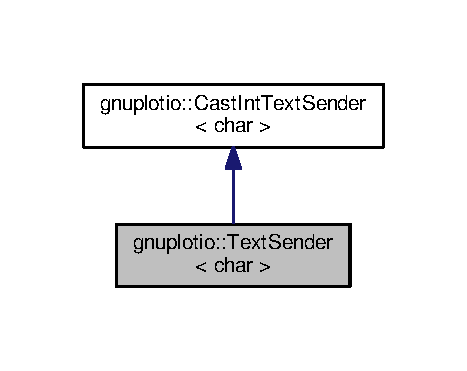
\includegraphics[width=224pt]{structgnuplotio_1_1_text_sender_3_01char_01_4__inherit__graph}
\end{center}
\end{figure}


Collaboration diagram for gnuplotio\+:\+:Text\+Sender$<$ char $>$\+:
\nopagebreak
\begin{figure}[H]
\begin{center}
\leavevmode
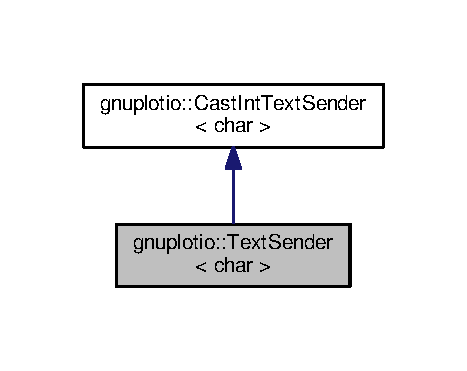
\includegraphics[width=224pt]{structgnuplotio_1_1_text_sender_3_01char_01_4__coll__graph}
\end{center}
\end{figure}
\subsection*{Additional Inherited Members}


The documentation for this struct was generated from the following file\+:\begin{DoxyCompactItemize}
\item 
/home/rajshinde/\+G\+M\+O\+C\+K/\+Robot\+\_\+\+Controller\+\_\+\+Module/include/gnuplot-\/iostream.\+h\end{DoxyCompactItemize}

\hypertarget{structgnuplotio_1_1_text_sender_3_01double_01_4}{}\section{gnuplotio\+:\+:Text\+Sender$<$ double $>$ Struct Template Reference}
\label{structgnuplotio_1_1_text_sender_3_01double_01_4}\index{gnuplotio\+::\+Text\+Sender$<$ double $>$@{gnuplotio\+::\+Text\+Sender$<$ double $>$}}


Inheritance diagram for gnuplotio\+:\+:Text\+Sender$<$ double $>$\+:
\nopagebreak
\begin{figure}[H]
\begin{center}
\leavevmode
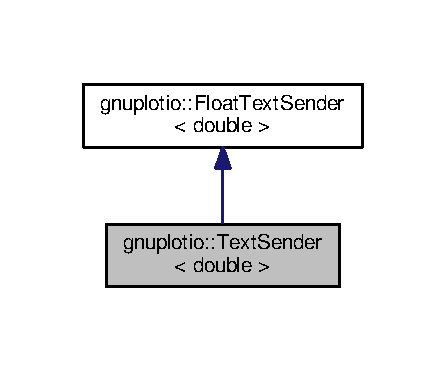
\includegraphics[width=214pt]{structgnuplotio_1_1_text_sender_3_01double_01_4__inherit__graph}
\end{center}
\end{figure}


Collaboration diagram for gnuplotio\+:\+:Text\+Sender$<$ double $>$\+:
\nopagebreak
\begin{figure}[H]
\begin{center}
\leavevmode
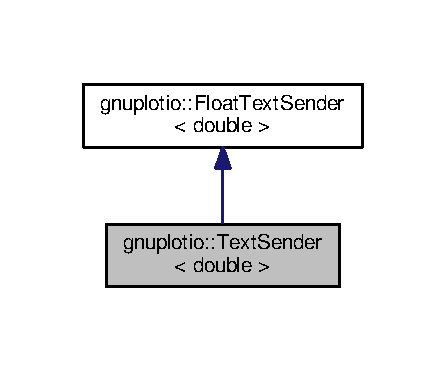
\includegraphics[width=214pt]{structgnuplotio_1_1_text_sender_3_01double_01_4__coll__graph}
\end{center}
\end{figure}
\subsection*{Additional Inherited Members}


The documentation for this struct was generated from the following file\+:\begin{DoxyCompactItemize}
\item 
/home/rajshinde/\+G\+M\+O\+C\+K/\+Robot\+\_\+\+Controller\+\_\+\+Module/include/gnuplot-\/iostream.\+h\end{DoxyCompactItemize}

\hypertarget{structgnuplotio_1_1_text_sender_3_01float_01_4}{}\section{gnuplotio\+:\+:Text\+Sender$<$ float $>$ Struct Template Reference}
\label{structgnuplotio_1_1_text_sender_3_01float_01_4}\index{gnuplotio\+::\+Text\+Sender$<$ float $>$@{gnuplotio\+::\+Text\+Sender$<$ float $>$}}


Inheritance diagram for gnuplotio\+:\+:Text\+Sender$<$ float $>$\+:
\nopagebreak
\begin{figure}[H]
\begin{center}
\leavevmode
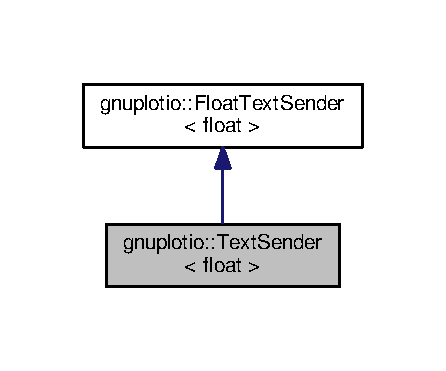
\includegraphics[width=214pt]{structgnuplotio_1_1_text_sender_3_01float_01_4__inherit__graph}
\end{center}
\end{figure}


Collaboration diagram for gnuplotio\+:\+:Text\+Sender$<$ float $>$\+:
\nopagebreak
\begin{figure}[H]
\begin{center}
\leavevmode
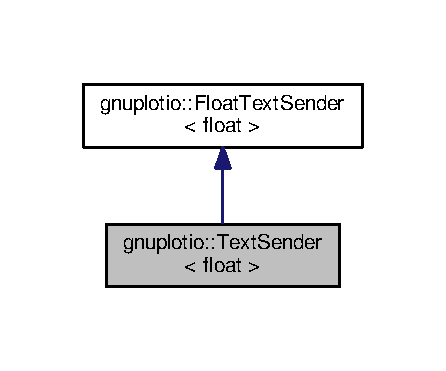
\includegraphics[width=214pt]{structgnuplotio_1_1_text_sender_3_01float_01_4__coll__graph}
\end{center}
\end{figure}
\subsection*{Additional Inherited Members}


The documentation for this struct was generated from the following file\+:\begin{DoxyCompactItemize}
\item 
/home/rajshinde/\+G\+M\+O\+C\+K/\+Robot\+\_\+\+Controller\+\_\+\+Module/include/gnuplot-\/iostream.\+h\end{DoxyCompactItemize}

\hypertarget{structgnuplotio_1_1_text_sender_3_01long_01double_01_4}{}\section{gnuplotio\+:\+:Text\+Sender$<$ long double $>$ Struct Template Reference}
\label{structgnuplotio_1_1_text_sender_3_01long_01double_01_4}\index{gnuplotio\+::\+Text\+Sender$<$ long double $>$@{gnuplotio\+::\+Text\+Sender$<$ long double $>$}}


Inheritance diagram for gnuplotio\+:\+:Text\+Sender$<$ long double $>$\+:
\nopagebreak
\begin{figure}[H]
\begin{center}
\leavevmode
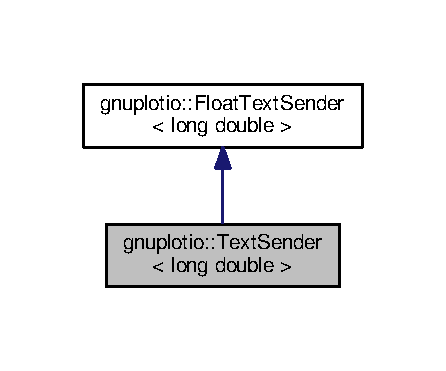
\includegraphics[width=214pt]{structgnuplotio_1_1_text_sender_3_01long_01double_01_4__inherit__graph}
\end{center}
\end{figure}


Collaboration diagram for gnuplotio\+:\+:Text\+Sender$<$ long double $>$\+:
\nopagebreak
\begin{figure}[H]
\begin{center}
\leavevmode
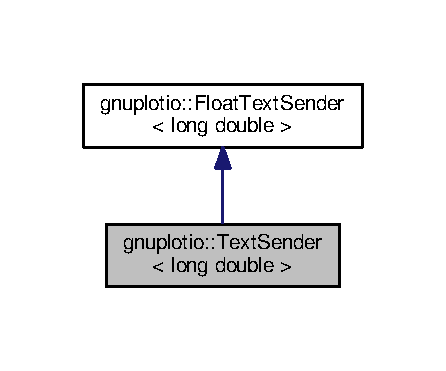
\includegraphics[width=214pt]{structgnuplotio_1_1_text_sender_3_01long_01double_01_4__coll__graph}
\end{center}
\end{figure}
\subsection*{Additional Inherited Members}


The documentation for this struct was generated from the following file\+:\begin{DoxyCompactItemize}
\item 
/home/rajshinde/\+G\+M\+O\+C\+K/\+Robot\+\_\+\+Controller\+\_\+\+Module/include/gnuplot-\/iostream.\+h\end{DoxyCompactItemize}

\hypertarget{structgnuplotio_1_1_text_sender_3_01signed_01char_01_4}{}\section{gnuplotio\+:\+:Text\+Sender$<$ signed char $>$ Struct Template Reference}
\label{structgnuplotio_1_1_text_sender_3_01signed_01char_01_4}\index{gnuplotio\+::\+Text\+Sender$<$ signed char $>$@{gnuplotio\+::\+Text\+Sender$<$ signed char $>$}}


Inheritance diagram for gnuplotio\+:\+:Text\+Sender$<$ signed char $>$\+:
\nopagebreak
\begin{figure}[H]
\begin{center}
\leavevmode
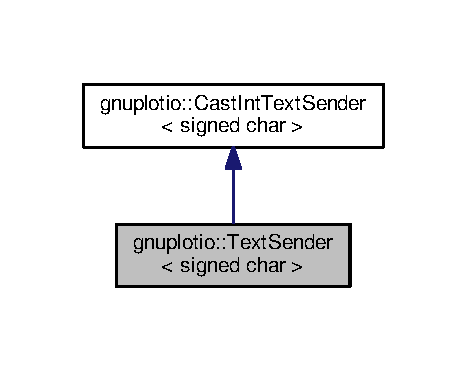
\includegraphics[width=224pt]{structgnuplotio_1_1_text_sender_3_01signed_01char_01_4__inherit__graph}
\end{center}
\end{figure}


Collaboration diagram for gnuplotio\+:\+:Text\+Sender$<$ signed char $>$\+:
\nopagebreak
\begin{figure}[H]
\begin{center}
\leavevmode
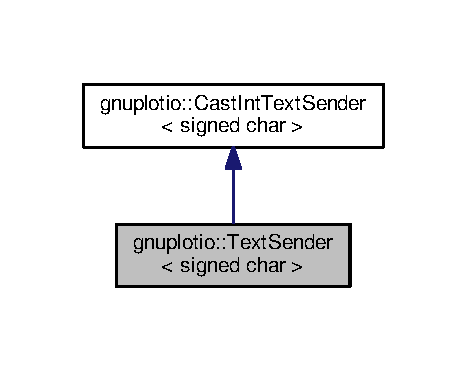
\includegraphics[width=224pt]{structgnuplotio_1_1_text_sender_3_01signed_01char_01_4__coll__graph}
\end{center}
\end{figure}
\subsection*{Additional Inherited Members}


The documentation for this struct was generated from the following file\+:\begin{DoxyCompactItemize}
\item 
/home/rajshinde/\+G\+M\+O\+C\+K/\+Robot\+\_\+\+Controller\+\_\+\+Module/include/gnuplot-\/iostream.\+h\end{DoxyCompactItemize}

\hypertarget{structgnuplotio_1_1_text_sender_3_01std_1_1complex_3_01_t_01_4_01_4}{}\section{gnuplotio\+:\+:Text\+Sender$<$ std\+:\+:complex$<$ T $>$ $>$ Struct Template Reference}
\label{structgnuplotio_1_1_text_sender_3_01std_1_1complex_3_01_t_01_4_01_4}\index{gnuplotio\+::\+Text\+Sender$<$ std\+::complex$<$ T $>$ $>$@{gnuplotio\+::\+Text\+Sender$<$ std\+::complex$<$ T $>$ $>$}}
\subsection*{Static Public Member Functions}
\begin{DoxyCompactItemize}
\item 
static void {\bfseries send} (std\+::ostream \&stream, const std\+::complex$<$ T $>$ \&v)\hypertarget{structgnuplotio_1_1_text_sender_3_01std_1_1complex_3_01_t_01_4_01_4_ad524aa3e121d0ebd66346d77f1fd5a1c}{}\label{structgnuplotio_1_1_text_sender_3_01std_1_1complex_3_01_t_01_4_01_4_ad524aa3e121d0ebd66346d77f1fd5a1c}

\end{DoxyCompactItemize}


The documentation for this struct was generated from the following file\+:\begin{DoxyCompactItemize}
\item 
/home/rajshinde/\+G\+M\+O\+C\+K/\+Robot\+\_\+\+Controller\+\_\+\+Module/include/gnuplot-\/iostream.\+h\end{DoxyCompactItemize}

\hypertarget{structgnuplotio_1_1_text_sender_3_01std_1_1pair_3_01_t_00_01_u_01_4_01_4}{}\section{gnuplotio\+:\+:Text\+Sender$<$ std\+:\+:pair$<$ T, U $>$ $>$ Struct Template Reference}
\label{structgnuplotio_1_1_text_sender_3_01std_1_1pair_3_01_t_00_01_u_01_4_01_4}\index{gnuplotio\+::\+Text\+Sender$<$ std\+::pair$<$ T, U $>$ $>$@{gnuplotio\+::\+Text\+Sender$<$ std\+::pair$<$ T, U $>$ $>$}}
\subsection*{Static Public Member Functions}
\begin{DoxyCompactItemize}
\item 
static void {\bfseries send} (std\+::ostream \&stream, const std\+::pair$<$ T, U $>$ \&v)\hypertarget{structgnuplotio_1_1_text_sender_3_01std_1_1pair_3_01_t_00_01_u_01_4_01_4_ae1f3a6ffd8a60bb73d787578327154d1}{}\label{structgnuplotio_1_1_text_sender_3_01std_1_1pair_3_01_t_00_01_u_01_4_01_4_ae1f3a6ffd8a60bb73d787578327154d1}

\end{DoxyCompactItemize}


The documentation for this struct was generated from the following file\+:\begin{DoxyCompactItemize}
\item 
/home/rajshinde/\+G\+M\+O\+C\+K/\+Robot\+\_\+\+Controller\+\_\+\+Module/include/gnuplot-\/iostream.\+h\end{DoxyCompactItemize}

\hypertarget{structgnuplotio_1_1_text_sender_3_01_t_00_01typename_01boost_1_1enable__if_3_01boost_1_1mpl_1_1ad1ac3a3da167856c52be6ae54ba2c114}{}\section{gnuplotio\+:\+:Text\+Sender$<$ T, typename boost\+:\+:enable\+\_\+if$<$ boost\+:\+:mpl\+:\+:and\+\_\+$<$ is\+\_\+boost\+\_\+tuple$<$ T $>$, boost\+:\+:mpl\+:\+:not\+\_\+$<$ is\+\_\+boost\+\_\+tuple\+\_\+nulltype$<$ typename T\+:\+:tail\+\_\+type $>$ $>$ $>$ $>$\+:\+:type $>$ Struct Template Reference}
\label{structgnuplotio_1_1_text_sender_3_01_t_00_01typename_01boost_1_1enable__if_3_01boost_1_1mpl_1_1ad1ac3a3da167856c52be6ae54ba2c114}\index{gnuplotio\+::\+Text\+Sender$<$ T, typename boost\+::enable\+\_\+if$<$ boost\+::mpl\+::and\+\_\+$<$ is\+\_\+boost\+\_\+tuple$<$ T $>$, boost\+::mpl\+::not\+\_\+$<$ is\+\_\+boost\+\_\+tuple\+\_\+nulltype$<$ typename T\+::tail\+\_\+type $>$ $>$ $>$ $>$\+::type $>$@{gnuplotio\+::\+Text\+Sender$<$ T, typename boost\+::enable\+\_\+if$<$ boost\+::mpl\+::and\+\_\+$<$ is\+\_\+boost\+\_\+tuple$<$ T $>$, boost\+::mpl\+::not\+\_\+$<$ is\+\_\+boost\+\_\+tuple\+\_\+nulltype$<$ typename T\+::tail\+\_\+type $>$ $>$ $>$ $>$\+::type $>$}}
\subsection*{Static Public Member Functions}
\begin{DoxyCompactItemize}
\item 
static void {\bfseries send} (std\+::ostream \&stream, const T \&v)\hypertarget{structgnuplotio_1_1_text_sender_3_01_t_00_01typename_01boost_1_1enable__if_3_01boost_1_1mpl_1_1ad1ac3a3da167856c52be6ae54ba2c114_a57bf894398f70f08cd4bac18ee5cbf68}{}\label{structgnuplotio_1_1_text_sender_3_01_t_00_01typename_01boost_1_1enable__if_3_01boost_1_1mpl_1_1ad1ac3a3da167856c52be6ae54ba2c114_a57bf894398f70f08cd4bac18ee5cbf68}

\end{DoxyCompactItemize}


The documentation for this struct was generated from the following file\+:\begin{DoxyCompactItemize}
\item 
/home/rajshinde/\+G\+M\+O\+C\+K/\+Robot\+\_\+\+Controller\+\_\+\+Module/include/gnuplot-\/iostream.\+h\end{DoxyCompactItemize}

\hypertarget{structgnuplotio_1_1_text_sender_3_01_t_00_01typename_01boost_1_1enable__if_3_01boost_1_1mpl_1_1ab6d6864cc1b3ed233c9f15134694f953}{}\section{gnuplotio\+:\+:Text\+Sender$<$ T, typename boost\+:\+:enable\+\_\+if$<$ boost\+:\+:mpl\+:\+:and\+\_\+$<$ is\+\_\+boost\+\_\+tuple$<$ T $>$, is\+\_\+boost\+\_\+tuple\+\_\+nulltype$<$ typename T\+:\+:tail\+\_\+type $>$ $>$ $>$\+:\+:type $>$ Struct Template Reference}
\label{structgnuplotio_1_1_text_sender_3_01_t_00_01typename_01boost_1_1enable__if_3_01boost_1_1mpl_1_1ab6d6864cc1b3ed233c9f15134694f953}\index{gnuplotio\+::\+Text\+Sender$<$ T, typename boost\+::enable\+\_\+if$<$ boost\+::mpl\+::and\+\_\+$<$ is\+\_\+boost\+\_\+tuple$<$ T $>$, is\+\_\+boost\+\_\+tuple\+\_\+nulltype$<$ typename T\+::tail\+\_\+type $>$ $>$ $>$\+::type $>$@{gnuplotio\+::\+Text\+Sender$<$ T, typename boost\+::enable\+\_\+if$<$ boost\+::mpl\+::and\+\_\+$<$ is\+\_\+boost\+\_\+tuple$<$ T $>$, is\+\_\+boost\+\_\+tuple\+\_\+nulltype$<$ typename T\+::tail\+\_\+type $>$ $>$ $>$\+::type $>$}}
\subsection*{Static Public Member Functions}
\begin{DoxyCompactItemize}
\item 
static void {\bfseries send} (std\+::ostream \&stream, const T \&v)\hypertarget{structgnuplotio_1_1_text_sender_3_01_t_00_01typename_01boost_1_1enable__if_3_01boost_1_1mpl_1_1ab6d6864cc1b3ed233c9f15134694f953_a76a476180ea04c950c1cfdb71c556525}{}\label{structgnuplotio_1_1_text_sender_3_01_t_00_01typename_01boost_1_1enable__if_3_01boost_1_1mpl_1_1ab6d6864cc1b3ed233c9f15134694f953_a76a476180ea04c950c1cfdb71c556525}

\end{DoxyCompactItemize}


The documentation for this struct was generated from the following file\+:\begin{DoxyCompactItemize}
\item 
/home/rajshinde/\+G\+M\+O\+C\+K/\+Robot\+\_\+\+Controller\+\_\+\+Module/include/gnuplot-\/iostream.\+h\end{DoxyCompactItemize}

\hypertarget{structgnuplotio_1_1_text_sender_3_01unsigned_01char_01_4}{}\section{gnuplotio\+:\+:Text\+Sender$<$ unsigned char $>$ Struct Template Reference}
\label{structgnuplotio_1_1_text_sender_3_01unsigned_01char_01_4}\index{gnuplotio\+::\+Text\+Sender$<$ unsigned char $>$@{gnuplotio\+::\+Text\+Sender$<$ unsigned char $>$}}


Inheritance diagram for gnuplotio\+:\+:Text\+Sender$<$ unsigned char $>$\+:
\nopagebreak
\begin{figure}[H]
\begin{center}
\leavevmode
\includegraphics[width=224pt]{structgnuplotio_1_1_text_sender_3_01unsigned_01char_01_4__inherit__graph}
\end{center}
\end{figure}


Collaboration diagram for gnuplotio\+:\+:Text\+Sender$<$ unsigned char $>$\+:
\nopagebreak
\begin{figure}[H]
\begin{center}
\leavevmode
\includegraphics[width=224pt]{structgnuplotio_1_1_text_sender_3_01unsigned_01char_01_4__coll__graph}
\end{center}
\end{figure}
\subsection*{Additional Inherited Members}


The documentation for this struct was generated from the following file\+:\begin{DoxyCompactItemize}
\item 
/home/rajshinde/\+G\+M\+O\+C\+K/\+Robot\+\_\+\+Controller\+\_\+\+Module/include/gnuplot-\/iostream.\+h\end{DoxyCompactItemize}

\hypertarget{structgnuplotio_1_1_mode_auto_decoder_3_01_t_00_01typename_01boost_1_1enable__if__c_3_01_07_arra33ab7f3325313485a7f29355d9a819fc}{}\section{gnuplotio\+:\+:type$<$ T $>$ Struct Template Reference}
\label{structgnuplotio_1_1_mode_auto_decoder_3_01_t_00_01typename_01boost_1_1enable__if__c_3_01_07_arra33ab7f3325313485a7f29355d9a819fc}\index{gnuplotio\+::type$<$ T $>$@{gnuplotio\+::type$<$ T $>$}}
\subsection*{Public Types}
\begin{DoxyCompactItemize}
\item 
typedef \hyperlink{structgnuplotio_1_1_mode2_d}{Mode2D} {\bfseries mode}\hypertarget{structgnuplotio_1_1_mode_auto_decoder_3_01_t_00_01typename_01boost_1_1enable__if__c_3_01_07_arra33ab7f3325313485a7f29355d9a819fc_a1574a7286cee13eedaeca8f40e7d0527}{}\label{structgnuplotio_1_1_mode_auto_decoder_3_01_t_00_01typename_01boost_1_1enable__if__c_3_01_07_arra33ab7f3325313485a7f29355d9a819fc_a1574a7286cee13eedaeca8f40e7d0527}

\end{DoxyCompactItemize}


The documentation for this struct was generated from the following file\+:\begin{DoxyCompactItemize}
\item 
/home/rajshinde/\+G\+M\+O\+C\+K/\+Robot\+\_\+\+Controller\+\_\+\+Module/include/gnuplot-\/iostream.\+h\end{DoxyCompactItemize}

\hypertarget{structgnuplotio_1_1_mode_auto_decoder_3_01_t_00_01typename_01boost_1_1enable__if__c_3_01_07_arra8faa7fb46cef74a29a23f22c000e4a99}{}\section{gnuplotio\+:\+:type$<$ T $>$ Struct Template Reference}
\label{structgnuplotio_1_1_mode_auto_decoder_3_01_t_00_01typename_01boost_1_1enable__if__c_3_01_07_arra8faa7fb46cef74a29a23f22c000e4a99}\index{gnuplotio\+::type$<$ T $>$@{gnuplotio\+::type$<$ T $>$}}
\subsection*{Public Types}
\begin{DoxyCompactItemize}
\item 
typedef \hyperlink{structgnuplotio_1_1_mode1_d_unwrap}{Mode1\+D\+Unwrap} {\bfseries mode}\hypertarget{structgnuplotio_1_1_mode_auto_decoder_3_01_t_00_01typename_01boost_1_1enable__if__c_3_01_07_arra8faa7fb46cef74a29a23f22c000e4a99_a9c16f714b67e1c4b38e5c7ff956e8acc}{}\label{structgnuplotio_1_1_mode_auto_decoder_3_01_t_00_01typename_01boost_1_1enable__if__c_3_01_07_arra8faa7fb46cef74a29a23f22c000e4a99_a9c16f714b67e1c4b38e5c7ff956e8acc}

\end{DoxyCompactItemize}


The documentation for this struct was generated from the following file\+:\begin{DoxyCompactItemize}
\item 
/home/rajshinde/\+G\+M\+O\+C\+K/\+Robot\+\_\+\+Controller\+\_\+\+Module/include/gnuplot-\/iostream.\+h\end{DoxyCompactItemize}

\hypertarget{structgnuplotio_1_1_mode_auto_decoder_3_01_t_00_01typename_01boost_1_1enable__if__c_3_01_07_arraea646779afc1e35efaeffcebe81e18a0}{}\section{gnuplotio\+:\+:type$<$ T $>$ Struct Template Reference}
\label{structgnuplotio_1_1_mode_auto_decoder_3_01_t_00_01typename_01boost_1_1enable__if__c_3_01_07_arraea646779afc1e35efaeffcebe81e18a0}\index{gnuplotio\+::type$<$ T $>$@{gnuplotio\+::type$<$ T $>$}}
\subsection*{Public Types}
\begin{DoxyCompactItemize}
\item 
typedef \hyperlink{structgnuplotio_1_1_mode1_d}{Mode1D} {\bfseries mode}\hypertarget{structgnuplotio_1_1_mode_auto_decoder_3_01_t_00_01typename_01boost_1_1enable__if__c_3_01_07_arraea646779afc1e35efaeffcebe81e18a0_a17dc2e2ec9d21833a8bd6f1a67e32e48}{}\label{structgnuplotio_1_1_mode_auto_decoder_3_01_t_00_01typename_01boost_1_1enable__if__c_3_01_07_arraea646779afc1e35efaeffcebe81e18a0_a17dc2e2ec9d21833a8bd6f1a67e32e48}

\end{DoxyCompactItemize}


The documentation for this struct was generated from the following file\+:\begin{DoxyCompactItemize}
\item 
/home/rajshinde/\+G\+M\+O\+C\+K/\+Robot\+\_\+\+Controller\+\_\+\+Module/include/gnuplot-\/iostream.\+h\end{DoxyCompactItemize}

\hypertarget{classgnuplotio_1_1_vec_of_range}{}\section{gnuplotio\+:\+:Vec\+Of\+Range$<$ RT $>$ Class Template Reference}
\label{classgnuplotio_1_1_vec_of_range}\index{gnuplotio\+::\+Vec\+Of\+Range$<$ R\+T $>$@{gnuplotio\+::\+Vec\+Of\+Range$<$ R\+T $>$}}
\subsection*{Public Types}
\begin{DoxyCompactItemize}
\item 
typedef std\+::vector$<$ typename R\+T\+::value\+\_\+type $>$ {\bfseries value\+\_\+type}\hypertarget{classgnuplotio_1_1_vec_of_range_aed503f2f8d8ed71b303f2db26872bafd}{}\label{classgnuplotio_1_1_vec_of_range_aed503f2f8d8ed71b303f2db26872bafd}

\item 
typedef \hyperlink{classgnuplotio_1_1_vec_of_range}{Vec\+Of\+Range}$<$ typename R\+T\+::subiter\+\_\+type $>$ {\bfseries subiter\+\_\+type}\hypertarget{classgnuplotio_1_1_vec_of_range_a4cfae20b9797febceffafec3415b52db}{}\label{classgnuplotio_1_1_vec_of_range_a4cfae20b9797febceffafec3415b52db}

\end{DoxyCompactItemize}
\subsection*{Public Member Functions}
\begin{DoxyCompactItemize}
\item 
{\bfseries Vec\+Of\+Range} (const std\+::vector$<$ RT $>$ \&\+\_\+rvec)\hypertarget{classgnuplotio_1_1_vec_of_range_a81e04f9ab4b8641d69df61f695e97e34}{}\label{classgnuplotio_1_1_vec_of_range_a81e04f9ab4b8641d69df61f695e97e34}

\item 
bool {\bfseries is\+\_\+end} () const \hypertarget{classgnuplotio_1_1_vec_of_range_a2beef61aa5b150db9af86b1de2edcb22}{}\label{classgnuplotio_1_1_vec_of_range_a2beef61aa5b150db9af86b1de2edcb22}

\item 
void {\bfseries inc} ()\hypertarget{classgnuplotio_1_1_vec_of_range_a2e5371ab6c88994e3fc6f12324783e1c}{}\label{classgnuplotio_1_1_vec_of_range_a2e5371ab6c88994e3fc6f12324783e1c}

\item 
value\+\_\+type {\bfseries deref} () const \hypertarget{classgnuplotio_1_1_vec_of_range_aa33d4275110fb0d5d76f56199381740f}{}\label{classgnuplotio_1_1_vec_of_range_aa33d4275110fb0d5d76f56199381740f}

\item 
\hyperlink{classgnuplotio_1_1_vec_of_range}{subiter\+\_\+type} {\bfseries deref\+\_\+subiter} () const \hypertarget{classgnuplotio_1_1_vec_of_range_a2f2ff571b1ef737f60bb0094e1dc221e}{}\label{classgnuplotio_1_1_vec_of_range_a2f2ff571b1ef737f60bb0094e1dc221e}

\end{DoxyCompactItemize}
\subsection*{Static Public Attributes}
\begin{DoxyCompactItemize}
\item 
static const bool {\bfseries is\+\_\+container} = R\+T\+::is\+\_\+container\hypertarget{classgnuplotio_1_1_vec_of_range_a8725d4907d46575dddb7152f1f1d1f66}{}\label{classgnuplotio_1_1_vec_of_range_a8725d4907d46575dddb7152f1f1d1f66}

\item 
static const bool {\bfseries allow\+\_\+auto\+\_\+unwrap} = false\hypertarget{classgnuplotio_1_1_vec_of_range_a19d87e61a7854f9e22d3dd8a94f79500}{}\label{classgnuplotio_1_1_vec_of_range_a19d87e61a7854f9e22d3dd8a94f79500}

\end{DoxyCompactItemize}
\subsection*{Friends}
\begin{DoxyCompactItemize}
\item 
{\footnotesize template$<$typename T , typename Print\+Mode $>$ }\\void {\bfseries deref\+\_\+and\+\_\+print} (std\+::ostream \&, const \hyperlink{classgnuplotio_1_1_vec_of_range}{Vec\+Of\+Range}$<$ T $>$ \&, Print\+Mode)\hypertarget{classgnuplotio_1_1_vec_of_range_adafbfb0122b8e499d1af9c246f4ac288}{}\label{classgnuplotio_1_1_vec_of_range_adafbfb0122b8e499d1af9c246f4ac288}

\end{DoxyCompactItemize}


The documentation for this class was generated from the following file\+:\begin{DoxyCompactItemize}
\item 
/home/rajshinde/\+G\+M\+O\+C\+K/\+Robot\+\_\+\+Controller\+\_\+\+Module/include/gnuplot-\/iostream.\+h\end{DoxyCompactItemize}

\chapter{File Documentation}
\hypertarget{_navigation_8cpp}{}\section{/home/rajshinde/\+G\+M\+O\+C\+K/\+Robot\+\_\+\+Controller\+\_\+\+Module/app/\+Navigation.cpp File Reference}
\label{_navigation_8cpp}\index{/home/rajshinde/\+G\+M\+O\+C\+K/\+Robot\+\_\+\+Controller\+\_\+\+Module/app/\+Navigation.\+cpp@{/home/rajshinde/\+G\+M\+O\+C\+K/\+Robot\+\_\+\+Controller\+\_\+\+Module/app/\+Navigation.\+cpp}}


Mid Term Project.  


{\ttfamily \#include $<$time.\+h$>$}\\*
{\ttfamily \#include $<$../include/gnuplot-\/iostream.\+h$>$}\\*
{\ttfamily \#include $<$iostream$>$}\\*
{\ttfamily \#include $<$fstream$>$}\\*
{\ttfamily \#include $<$vector$>$}\\*
{\ttfamily \#include $<$Navigation.\+hpp$>$}\\*
{\ttfamily \#include $<$Steer\+Algorithm.\+hpp$>$}\\*
Include dependency graph for Navigation.\+cpp\+:
\nopagebreak
\begin{figure}[H]
\begin{center}
\leavevmode
\includegraphics[width=350pt]{_navigation_8cpp__incl}
\end{center}
\end{figure}


\subsection{Detailed Description}
Mid Term Project. 

\begin{DoxyCopyright}{Copyright}
M\+IT License, Copyright © 2019 Raj Shinde
\end{DoxyCopyright}
\begin{DoxyAuthor}{Author}
Sprint-\/1 Raj Shinde-\/ driver and Prasheel Renkuntla-\/ navigator 

Sprint-\/2 Prasheel Renkuntla-\/ driver and Raj Shinde-\/ navigator 
\end{DoxyAuthor}
\begin{DoxyDate}{Date}
11/24/2019 
\end{DoxyDate}
\begin{DoxyVersion}{Version}
6.\+0 
\end{DoxyVersion}
\hypertarget{_steer_algorithm_8cpp_Implements}{}\subsection{Ackermann on P\+I\+D control}\label{_steer_algorithm_8cpp_Implements}

\hypertarget{_steer_algorithm_8cpp}{}\section{/home/rajshinde/\+G\+M\+O\+C\+K/\+Robot\+\_\+\+Controller\+\_\+\+Module/app/\+Steer\+Algorithm.cpp File Reference}
\label{_steer_algorithm_8cpp}\index{/home/rajshinde/\+G\+M\+O\+C\+K/\+Robot\+\_\+\+Controller\+\_\+\+Module/app/\+Steer\+Algorithm.\+cpp@{/home/rajshinde/\+G\+M\+O\+C\+K/\+Robot\+\_\+\+Controller\+\_\+\+Module/app/\+Steer\+Algorithm.\+cpp}}


Mid Term Project.  


{\ttfamily \#include $<$iostream$>$}\\*
{\ttfamily \#include $<$cmath$>$}\\*
{\ttfamily \#include \char`\"{}Steer\+Algorithm.\+hpp\char`\"{}}\\*
Include dependency graph for Steer\+Algorithm.\+cpp\+:
\nopagebreak
\begin{figure}[H]
\begin{center}
\leavevmode
\includegraphics[width=314pt]{_steer_algorithm_8cpp__incl}
\end{center}
\end{figure}


\subsection{Detailed Description}
Mid Term Project. 

\begin{DoxyCopyright}{Copyright}
M\+IT License, Copyright © 2019 Raj Shinde
\end{DoxyCopyright}
\begin{DoxyAuthor}{Author}
Sprint-\/1 Raj Shinde-\/ driver and Prasheel Renkuntla-\/ navigator 

Sprint-\/2 Prasheel Renkuntla-\/ driver and Raj Shinde-\/ navigator 
\end{DoxyAuthor}
\begin{DoxyDate}{Date}
11/24/2019 
\end{DoxyDate}
\begin{DoxyVersion}{Version}
6.\+0 
\end{DoxyVersion}
\hypertarget{_steer_algorithm_8cpp_Implements}{}\subsection{Ackermann on P\+I\+D control}\label{_steer_algorithm_8cpp_Implements}

\hypertarget{_mock_navigation_8hpp}{}\section{/home/rajshinde/\+G\+M\+O\+C\+K/\+Robot\+\_\+\+Controller\+\_\+\+Module/include/\+Mock\+Navigation.hpp File Reference}
\label{_mock_navigation_8hpp}\index{/home/rajshinde/\+G\+M\+O\+C\+K/\+Robot\+\_\+\+Controller\+\_\+\+Module/include/\+Mock\+Navigation.\+hpp@{/home/rajshinde/\+G\+M\+O\+C\+K/\+Robot\+\_\+\+Controller\+\_\+\+Module/include/\+Mock\+Navigation.\+hpp}}


Mid Term Project.  


{\ttfamily \#include $<$gmock/gmock.\+h$>$}\\*
{\ttfamily \#include $<$vector$>$}\\*
{\ttfamily \#include $<$iostream$>$}\\*
{\ttfamily \#include \char`\"{}Navigation.\+hpp\char`\"{}}\\*
Include dependency graph for Mock\+Navigation.\+hpp\+:
\nopagebreak
\begin{figure}[H]
\begin{center}
\leavevmode
\includegraphics[width=350pt]{_mock_navigation_8hpp__incl}
\end{center}
\end{figure}
This graph shows which files directly or indirectly include this file\+:
\nopagebreak
\begin{figure}[H]
\begin{center}
\leavevmode
\includegraphics[width=225pt]{_mock_navigation_8hpp__dep__incl}
\end{center}
\end{figure}
\subsection*{Classes}
\begin{DoxyCompactItemize}
\item 
class \hyperlink{class_mock_navigation}{Mock\+Navigation}
\begin{DoxyCompactList}\small\item\em Mock \hyperlink{class_navigation}{Navigation} class. \end{DoxyCompactList}\end{DoxyCompactItemize}


\subsection{Detailed Description}
Mid Term Project. 

\begin{DoxyCopyright}{Copyright}
M\+IT License, Copyright © 2019 Raj Shinde
\end{DoxyCopyright}
\begin{DoxyAuthor}{Author}
Raj Shinde 
\end{DoxyAuthor}
\begin{DoxyDate}{Date}
11/24/2019 
\end{DoxyDate}
\begin{DoxyVersion}{Version}
7.\+0 
\end{DoxyVersion}
\hypertarget{_mock_navigation_8hpp_Mocked}{}\subsection{navigation class}\label{_mock_navigation_8hpp_Mocked}

\hypertarget{_navigation_8hpp}{}\section{/home/rajshinde/\+G\+M\+O\+C\+K/\+Robot\+\_\+\+Controller\+\_\+\+Module/include/\+Navigation.hpp File Reference}
\label{_navigation_8hpp}\index{/home/rajshinde/\+G\+M\+O\+C\+K/\+Robot\+\_\+\+Controller\+\_\+\+Module/include/\+Navigation.\+hpp@{/home/rajshinde/\+G\+M\+O\+C\+K/\+Robot\+\_\+\+Controller\+\_\+\+Module/include/\+Navigation.\+hpp}}


Mid Term Project.  


{\ttfamily \#include $<$vector$>$}\\*
{\ttfamily \#include $<$Steer\+Algorithm.\+hpp$>$}\\*
Include dependency graph for Navigation.\+hpp\+:
\nopagebreak
\begin{figure}[H]
\begin{center}
\leavevmode
\includegraphics[width=242pt]{_navigation_8hpp__incl}
\end{center}
\end{figure}
This graph shows which files directly or indirectly include this file\+:
\nopagebreak
\begin{figure}[H]
\begin{center}
\leavevmode
\includegraphics[width=350pt]{_navigation_8hpp__dep__incl}
\end{center}
\end{figure}
\subsection*{Classes}
\begin{DoxyCompactItemize}
\item 
class \hyperlink{class_navigation}{Navigation}
\begin{DoxyCompactList}\small\item\em Class \hyperlink{class_navigation}{Navigation} Contains the methods of steer Algorithm. \end{DoxyCompactList}\end{DoxyCompactItemize}


\subsection{Detailed Description}
Mid Term Project. 

\begin{DoxyCopyright}{Copyright}
M\+IT License, Copyright © 2019 Raj Shinde
\end{DoxyCopyright}
\begin{DoxyAuthor}{Author}
Sprint-\/1 Raj Shinde-\/ driver and Prasheel Renkuntla-\/ navigator 

Sprint-\/2 Prasheel Renkuntla-\/ driver and Raj Shinde-\/ navigator 
\end{DoxyAuthor}
\begin{DoxyDate}{Date}
11/24/2019 
\end{DoxyDate}
\begin{DoxyVersion}{Version}
6.\+0 
\end{DoxyVersion}
\hypertarget{_navigation_8hpp_Header}{}\subsection{file for Navigation through P\+I\+D control}\label{_navigation_8hpp_Header}

\hypertarget{_steer_algorithm_8hpp}{}\section{/home/rajshinde/\+G\+M\+O\+C\+K/\+Robot\+\_\+\+Controller\+\_\+\+Module/include/\+Steer\+Algorithm.hpp File Reference}
\label{_steer_algorithm_8hpp}\index{/home/rajshinde/\+G\+M\+O\+C\+K/\+Robot\+\_\+\+Controller\+\_\+\+Module/include/\+Steer\+Algorithm.\+hpp@{/home/rajshinde/\+G\+M\+O\+C\+K/\+Robot\+\_\+\+Controller\+\_\+\+Module/include/\+Steer\+Algorithm.\+hpp}}


Mid Term Project.  


This graph shows which files directly or indirectly include this file\+:
\nopagebreak
\begin{figure}[H]
\begin{center}
\leavevmode
\includegraphics[width=350pt]{_steer_algorithm_8hpp__dep__incl}
\end{center}
\end{figure}
\subsection*{Classes}
\begin{DoxyCompactItemize}
\item 
class \hyperlink{class_steer_algorithm}{Steer\+Algorithm}
\begin{DoxyCompactList}\small\item\em Class \hyperlink{class_steer_algorithm}{Steer\+Algorithm} contains the methods of the Steering Algorithm. \end{DoxyCompactList}\end{DoxyCompactItemize}


\subsection{Detailed Description}
Mid Term Project. 

\begin{DoxyCopyright}{Copyright}
M\+IT License, Copyright © 2019 Raj Shinde
\end{DoxyCopyright}
\begin{DoxyAuthor}{Author}
Sprint-\/1 Raj Shinde-\/ driver and Prasheel Renkuntla-\/ navigator 

Sprint-\/2 Prasheel Renkuntla-\/ driver and Raj Shinde-\/ navigator 
\end{DoxyAuthor}
\begin{DoxyDate}{Date}
11/25/2019 
\end{DoxyDate}
\begin{DoxyVersion}{Version}
6.\+0 
\end{DoxyVersion}
\hypertarget{_steer_algorithm_8hpp_Ackermann}{}\subsection{Steering Control Header file}\label{_steer_algorithm_8hpp_Ackermann}

\hypertarget{test_mock_navigation_8cpp}{}\section{/home/rajshinde/\+G\+M\+O\+C\+K/\+Robot\+\_\+\+Controller\+\_\+\+Module/test/test\+Mock\+Navigation.cpp File Reference}
\label{test_mock_navigation_8cpp}\index{/home/rajshinde/\+G\+M\+O\+C\+K/\+Robot\+\_\+\+Controller\+\_\+\+Module/test/test\+Mock\+Navigation.\+cpp@{/home/rajshinde/\+G\+M\+O\+C\+K/\+Robot\+\_\+\+Controller\+\_\+\+Module/test/test\+Mock\+Navigation.\+cpp}}


Mid Term Project.  


{\ttfamily \#include $<$gtest/gtest.\+h$>$}\\*
{\ttfamily \#include $<$gmock/gmock.\+h$>$}\\*
{\ttfamily \#include $<$iostream$>$}\\*
{\ttfamily \#include \char`\"{}Mock\+Navigation.\+hpp\char`\"{}}\\*
{\ttfamily \#include \char`\"{}Navigation.\+hpp\char`\"{}}\\*
Include dependency graph for test\+Mock\+Navigation.\+cpp\+:
\nopagebreak
\begin{figure}[H]
\begin{center}
\leavevmode
\includegraphics[width=350pt]{test_mock_navigation_8cpp__incl}
\end{center}
\end{figure}
\subsection*{Functions}
\begin{DoxyCompactItemize}
\item 
\hyperlink{test_mock_navigation_8cpp_aa55b7a7a105e0f631cb0048e1114f74e}{T\+E\+ST} (\hyperlink{class_mock_navigation}{Mock\+Navigation}, test\+Get\+Kp)\hypertarget{test_mock_navigation_8cpp_aa55b7a7a105e0f631cb0048e1114f74e}{}\label{test_mock_navigation_8cpp_aa55b7a7a105e0f631cb0048e1114f74e}

\begin{DoxyCompactList}\small\item\em Test Kp and calculate using gmock. \end{DoxyCompactList}\item 
{\bfseries T\+E\+ST} (\hyperlink{class_mock_navigation}{Mock\+Navigation}, test\+Calculate)\hypertarget{test_mock_navigation_8cpp_a099fddf48e2fb6a9bbe7d6b38977b266}{}\label{test_mock_navigation_8cpp_a099fddf48e2fb6a9bbe7d6b38977b266}

\end{DoxyCompactItemize}


\subsection{Detailed Description}
Mid Term Project. 

\begin{DoxyCopyright}{Copyright}
M\+IT License, Copyright © 2019 Raj Shinde
\end{DoxyCopyright}
\begin{DoxyAuthor}{Author}
Raj Shinde 
\end{DoxyAuthor}
\begin{DoxyDate}{Date}
11/24/2019 
\end{DoxyDate}
\begin{DoxyVersion}{Version}
7.\+0 
\end{DoxyVersion}
\hypertarget{test_mock_navigation_8cpp_Test}{}\subsection{Mock\+Navigation}\label{test_mock_navigation_8cpp_Test}

\hypertarget{test_navigation_8cpp}{}\section{/home/rajshinde/\+G\+M\+O\+C\+K/\+Robot\+\_\+\+Controller\+\_\+\+Module/test/test\+Navigation.cpp File Reference}
\label{test_navigation_8cpp}\index{/home/rajshinde/\+G\+M\+O\+C\+K/\+Robot\+\_\+\+Controller\+\_\+\+Module/test/test\+Navigation.\+cpp@{/home/rajshinde/\+G\+M\+O\+C\+K/\+Robot\+\_\+\+Controller\+\_\+\+Module/test/test\+Navigation.\+cpp}}


Mid Term Project.  


{\ttfamily \#include $<$gtest/gtest.\+h$>$}\\*
{\ttfamily \#include $<$cstdlib$>$}\\*
{\ttfamily \#include $<$memory$>$}\\*
{\ttfamily \#include \char`\"{}Navigation.\+hpp\char`\"{}}\\*
Include dependency graph for test\+Navigation.\+cpp\+:
\nopagebreak
\begin{figure}[H]
\begin{center}
\leavevmode
\includegraphics[width=350pt]{test_navigation_8cpp__incl}
\end{center}
\end{figure}
\subsection*{Functions}
\begin{DoxyCompactItemize}
\item 
\hyperlink{test_navigation_8cpp_a093604a7433c91e9a41a6c486ff843b3}{T\+E\+ST} (\hyperlink{class_navigation}{Navigation}, test\+Set\+Pid)\hypertarget{test_navigation_8cpp_a093604a7433c91e9a41a6c486ff843b3}{}\label{test_navigation_8cpp_a093604a7433c91e9a41a6c486ff843b3}

\begin{DoxyCompactList}\small\item\em Test to check the set functions for kp\+\_\+,ki\+\_\+ and kd\+\_\+. \end{DoxyCompactList}\item 
\hyperlink{test_navigation_8cpp_a5c632ae16e5ba30ae35d75900430e15a}{T\+E\+ST} (\hyperlink{class_navigation}{Navigation}, test\+Get\+Pid)\hypertarget{test_navigation_8cpp_a5c632ae16e5ba30ae35d75900430e15a}{}\label{test_navigation_8cpp_a5c632ae16e5ba30ae35d75900430e15a}

\begin{DoxyCompactList}\small\item\em Test to check that values of kp\+\_\+,ki\+\_\+ and kd\+\_\+ are below 1 or not. \end{DoxyCompactList}\item 
\hyperlink{test_navigation_8cpp_acc7325d4d1f9e57e7d887a7af00c04b8}{T\+E\+ST} (\hyperlink{class_navigation}{Navigation}, test\+Convergence)\hypertarget{test_navigation_8cpp_acc7325d4d1f9e57e7d887a7af00c04b8}{}\label{test_navigation_8cpp_acc7325d4d1f9e57e7d887a7af00c04b8}

\begin{DoxyCompactList}\small\item\em Test to check the output of calculate function converges with the set\+Point and Heading. \end{DoxyCompactList}\item 
\hyperlink{test_navigation_8cpp_a279955e42b5475ff67d1558ecfdf116b}{T\+E\+ST} (\hyperlink{class_navigation}{Navigation}, graphs)\hypertarget{test_navigation_8cpp_a279955e42b5475ff67d1558ecfdf116b}{}\label{test_navigation_8cpp_a279955e42b5475ff67d1558ecfdf116b}

\begin{DoxyCompactList}\small\item\em Test to check the functions arclength and turn\+Time provide right length and time values. \end{DoxyCompactList}\end{DoxyCompactItemize}


\subsection{Detailed Description}
Mid Term Project. 

\begin{DoxyCopyright}{Copyright}
M\+IT License, Copyright © 2019 Raj Shinde
\end{DoxyCopyright}
\begin{DoxyAuthor}{Author}
Sprint-\/1 Raj Shinde-\/ driver and Prasheel Renkuntla-\/ navigator 

Sprint-\/2 Prasheel Renkuntla-\/ driver and Raj Shinde-\/ navigator 
\end{DoxyAuthor}
\begin{DoxyDate}{Date}
10/10/2019 
\end{DoxyDate}
\begin{DoxyVersion}{Version}
6.\+0 
\end{DoxyVersion}
\hypertarget{test_steer_algorithm_8cpp_Tests}{}\subsection{all files in module}\label{test_steer_algorithm_8cpp_Tests}

\hypertarget{test_steer_algorithm_8cpp}{}\section{/home/rajshinde/\+G\+M\+O\+C\+K/\+Robot\+\_\+\+Controller\+\_\+\+Module/test/test\+Steer\+Algorithm.cpp File Reference}
\label{test_steer_algorithm_8cpp}\index{/home/rajshinde/\+G\+M\+O\+C\+K/\+Robot\+\_\+\+Controller\+\_\+\+Module/test/test\+Steer\+Algorithm.\+cpp@{/home/rajshinde/\+G\+M\+O\+C\+K/\+Robot\+\_\+\+Controller\+\_\+\+Module/test/test\+Steer\+Algorithm.\+cpp}}


Mid Term Project.  


{\ttfamily \#include $<$gtest/gtest.\+h$>$}\\*
{\ttfamily \#include $<$cstdlib$>$}\\*
{\ttfamily \#include $<$memory$>$}\\*
{\ttfamily \#include \char`\"{}Steer\+Algorithm.\+hpp\char`\"{}}\\*
Include dependency graph for test\+Steer\+Algorithm.\+cpp\+:
\nopagebreak
\begin{figure}[H]
\begin{center}
\leavevmode
\includegraphics[width=350pt]{test_steer_algorithm_8cpp__incl}
\end{center}
\end{figure}
\subsection*{Functions}
\begin{DoxyCompactItemize}
\item 
\hyperlink{test_steer_algorithm_8cpp_a302ee9fe0ef08a6beaea103c911981ff}{T\+E\+ST} (\hyperlink{class_steer_algorithm}{Steer\+Algorithm}, test\+Corr\+Radius)\hypertarget{test_steer_algorithm_8cpp_a302ee9fe0ef08a6beaea103c911981ff}{}\label{test_steer_algorithm_8cpp_a302ee9fe0ef08a6beaea103c911981ff}

\begin{DoxyCompactList}\small\item\em Tests to check that the set functions works and the value of corr\+Radius in below setlimit. \end{DoxyCompactList}\item 
\hyperlink{test_steer_algorithm_8cpp_ab38a7e56f4e7418febe58d9daf9e4b58}{T\+E\+ST} (\hyperlink{class_steer_algorithm}{Steer\+Algorithm}, testwheel)\hypertarget{test_steer_algorithm_8cpp_ab38a7e56f4e7418febe58d9daf9e4b58}{}\label{test_steer_algorithm_8cpp_ab38a7e56f4e7418febe58d9daf9e4b58}

\begin{DoxyCompactList}\small\item\em Tests to check if the wheel angles get resetted and the Ackeermann kinematic model is is properly implemented. \end{DoxyCompactList}\item 
\hyperlink{test_steer_algorithm_8cpp_a2e8c38dec883b8cfc46adb1e0cedb000}{T\+E\+ST} (\hyperlink{class_steer_algorithm}{Steer\+Algorithm}, test\+Calculations)\hypertarget{test_steer_algorithm_8cpp_a2e8c38dec883b8cfc46adb1e0cedb000}{}\label{test_steer_algorithm_8cpp_a2e8c38dec883b8cfc46adb1e0cedb000}

\begin{DoxyCompactList}\small\item\em Test to check the functions arclength and turn\+Time provide right length and time values. \end{DoxyCompactList}\end{DoxyCompactItemize}


\subsection{Detailed Description}
Mid Term Project. 

\begin{DoxyCopyright}{Copyright}
M\+IT License, Copyright © 2019 Raj Shinde
\end{DoxyCopyright}
\begin{DoxyAuthor}{Author}
Sprint-\/1 Raj Shinde-\/ driver and Prasheel Renkuntla-\/ navigator 

Sprint-\/2 Prasheel Renkuntla-\/ driver and Raj Shinde-\/ navigator 
\end{DoxyAuthor}
\begin{DoxyDate}{Date}
10/10/2019 
\end{DoxyDate}
\begin{DoxyVersion}{Version}
6.\+0 
\end{DoxyVersion}
\hypertarget{test_steer_algorithm_8cpp_Tests}{}\subsection{all files in module}\label{test_steer_algorithm_8cpp_Tests}

%--- End generated contents ---

% Index
\backmatter
\newpage
\phantomsection
\clearemptydoublepage
\addcontentsline{toc}{chapter}{Index}
\printindex

\end{document}
